%%%%%%%%%%%%%%%%%%%%%%%%%%%%%%%%%%%%%%%%%%%%%%%%%%%%%%%%%%%%%%%%%%%%%%%%%%%%%%%
%                       CARGA DE LA CLASE DE DOCUMENTO                        %
%                                                                             %
% Las opciones admisibles son:                                                %
%      12pt / 11pt            (tamaño de letra; no usar 10pt)                 %
%                                                                             %
% spanish                     (lengua principal del trabajo)                  %
%                                                                             %
% listoffigures               (El documento incluye un Índice de figuras)     %
% listoftables                (El documento incluye un Índice de tablas)      %
% listoflistings              (El documento incluye un Índice de códigos)     %
% listofquadres               (El documento incluye un Índice de cuadros)     %
%                                                                             %
%%%%%%%%%%%%%%%%%%%%%%%%%%%%%%%%%%%%%%%%%%%%%%%%%%%%%%%%%%%%%%%%%%%%%%%%%%%%%%%

\documentclass[12pt,spanish]{plantilla_proyecto}

%%%%%%%%%%%%%%%%%%%%%%%%%%%%%%%%%%%%%%%%%%%%%%%%%%%%%%%%%%%%%%%%%%%%%%%%%%%%%%%
%                     CODIFICACIÓN DEL ARCHIVO FUENTE                         %
%                                                                             %
%    Windows usa normalmente 'ansinew'                                        %
%    En Linux es posible que sea 'latin1' o 'latin9'                          %
%    Pero lo más recomendable es usar utf8 (Unicode 8)                        %
%                                          (si su editor lo permite)          % 
%%%%%%%%%%%%%%%%%%%%%%%%%%%%%%%%%%%%%%%%%%%%%%%%%%%%%%%%%%%%%%%%%%%%%%%%%%%%%%%

\usepackage[utf8]{inputenc} 
%%%%%%%%%%%%%%%%%%%%%%%%%%%%%%%%%%%%%%%%%%%%%%%%%%%%%%%%%%%%%%%%%%%%%
% Para conseguir que la tabla de contenido no salga en rojo
%%%%%%%%%%%%%%%%%%%%%%%%%%%%%%%%%%%%%%%%%%%%%%%%%%%%%%%%%%%%%%%%%%%%%

\hypersetup{ colorlinks=true, linkcolor=black, urlcolor=cyan, }

%%%%%%%%%%%%%%%%%%%%%%%%%%%%%%%%%%%%%%%%%%%%%%%%%%%%%%%%%%%%%%%%%%%%%%%%%%%%%%%
%                        OTROS PAQUETES Y DEFINICIONES                        %
%                                                                             %
% Cargue aquí los paquetes que necesite y declare los comandos y entornos     %
%                                          (esta sección puede estar vacía)   %
%%%%%%%%%%%%%%%%%%%%%%%%%%%%%%%%%%%%%%%%%%%%%%%%%%%%%%%%%%%%%%%%%%%%%%%%%%%%%%%


% Evita que los entornos se partan, necesario en algunos capítulos
\usepackage{needspace}
% Soporte para inclusión de imágenes
\usepackage{graphicx}
% Permitir posicionamiento exacto de figuras
\usepackage{float}
% Mejoras para tablas con texto que debe ajustarse
\usepackage{tabularx}
\usepackage{ragged2e}
% Permite partir palabras largas (ej. identificadores con guiones y subrayados)
\usepackage{seqsplit}

% Entorno visual para definiciones formales
\usepackage{mdframed}
\newmdenv[
    linecolor=black,
    backgroundcolor=gray!15,
    innertopmargin=6pt,
    innerbottommargin=6pt,
    innerrightmargin=6pt,
    innerleftmargin=6pt,
    skipabove=8pt,
    skipbelow=8pt
]{definicionbox}
\newenvironment{definicion}[1][]
    {\begin{definicionbox}\itshape}
    {\end{definicionbox}}


%%%%%%%%%%%%%%%%%%%%%%%%%%%%%%%%%%%%%%%%%%%%%%%%%%%%%%%%%%%%%%%%%%%%%%%%%%%%%%%
%                        DATOS DEL TRABAJO                                    %
%                                                                             %
% título, alumno, tutor y curso académico                                     %
%%%%%%%%%%%%%%%%%%%%%%%%%%%%%%%%%%%%%%%%%%%%%%%%%%%%%%%%%%%%%%%%%%%%%%%%%%%%%%%

% TODO: Ajustar título del nuevo trabajo

\title{Libreta de Estudio \\ Redes Industriales}
\author{Francisco Nortes Novikov \\ Mario Martínez Carneros}
\tutor{Guillermo Lenin Lemus Zúñiga}

%%%%%%%%%%%%%%%%%%%%%%%%%%%%%%%%%%%%%%%%%%%%%%%%%%%%%%%%%%%%%%%%%%%%%%%%%%%%%%%
%                           PALABRAS CLAVE                                    %
%                                                                             %
% Incluya aquí únicamente las palabras clave en español                       %
%%%%%%%%%%%%%%%%%%%%%%%%%%%%%%%%%%%%%%%%%%%%%%%%%%%%%%%%%%%%%%%%%%%%%%%%%%%%%%%

\keywords{TODO: palabra clave 1, palabra clave 2, palabra clave 3}

%%%%%%%%%%%%%%%%%%%%%%%%%%%%%%%%%%%%%%%%%%%%%%%%%%%%%%%%%%%%%%%%%%%%%%%%%%%%%%%
%                              INICIO DEL DOCUMENTO                           %
%%%%%%%%%%%%%%%%%%%%%%%%%%%%%%%%%%%%%%%%%%%%%%%%%%%%%%%%%%%%%%%%%%%%%%%%%%%%%%%

\begin{document}

%%%%%%%%%%%%%%%%%%%%%%%%%%%%%%%%%%%%%%%%%%%%%%%%%%%%%%%%%%%%%%%%%%%%%%%%%%%%%%%
%                                ÍNDICES                                      %
%%%%%%%%%%%%%%%%%%%%%%%%%%%%%%%%%%%%%%%%%%%%%%%%%%%%%%%%%%%%%%%%%%%%%%%%%%%%%%%

\setcounter{tocdepth}{1}
\makeindexes

%%%%%%%%%%%%%%%%%%%%%%%%%%%%%%%%%%%%%%%%%%%%%%%%%%%%%%%%%%%%%%%%%%%%%%%%%%%%%%%
%                           RESUMEN DEL TRABAJO                               %
%%%%%%%%%%%%%%%%%%%%%%%%%%%%%%%%%%%%%%%%%%%%%%%%%%%%%%%%%%%%%%%%%%%%%%%%%%%%%%%

\begin{abstract}
En este portafolio se exponen los resúmenes de los temas vistos en clase de la asignatura Redes Industriales, abarcando desde los fundamentos de comunicación serie y redes inalámbricas hasta protocolos de bus industrial, TCP/IP, encaminamiento y redes de área local. Se incluyen también las prácticas realizadas en el laboratorio con ESP32-S3 y Cisco Packet Tracer. Adicionalmente, se presenta el trabajo académico sobre un proceso industrial automatizado con ESP32, Arduino UNO y MQTT, junto con el diseño de su red corporativa. Todo el contenido se basa en el material docente de Lemus Zúñiga, G. L. disponible en Poliformat.
\end{abstract}

%%%%%%%%%%%%%%%%%%%%%%%%%%%%%%%%%%%%%%%%%%%%%%%%%%%%%%%%%%%%%%%%%%%%%%%%%%%%%%%
%                              CONTENIDO DEL TRABAJO                          %
%%%%%%%%%%%%%%%%%%%%%%%%%%%%%%%%%%%%%%%%%%%%%%%%%%%%%%%%%%%%%%%%%%%%%%%%%%%%%%%

\mainmatter

% UNIDADES / TEMAS
%%%%%%%%%%%%%%%%%%%%%%%%%%%%%%%%%%%%%%%%%%%%%%%%%%%%%%%%%%%%%%%%%%%%%%%%%%%%%%%
%                         UNIDAD 1: COMUNICACIÓN SERIE                        %
%%%%%%%%%%%%%%%%%%%%%%%%%%%%%%%%%%%%%%%%%%%%%%%%%%%%%%%%%%%%%%%%%%%%%%%%%%%%%%%

\chapter{Unidad 1: Comunicación Serie}

\section{¿Por qué comunicamos dispositivos?}

En cualquier sistema industrial moderno, los componentes necesitan intercambiar información: un sensor debe enviar una medida a un controlador, un PLC debe ordenar un movimiento a un motor, o un ordenador debe supervisar el estado de toda una planta. Esta necesidad de compartir datos entre dispositivos electrónicos es el origen de las comunicaciones digitales.

A lo largo de la historia, los ingenieros han buscado formas cada vez más eficientes de transmitir información. Desde el telégrafo de Samuel Morse (1844), que enviaba puntos y rayas por un único cable, hasta las redes industriales actuales que mueven gigabytes por segundo, el principio fundamental es el mismo: codificar información, transportarla por un medio físico y decodificarla en el destino.

\begin{figure}[H]
\centering
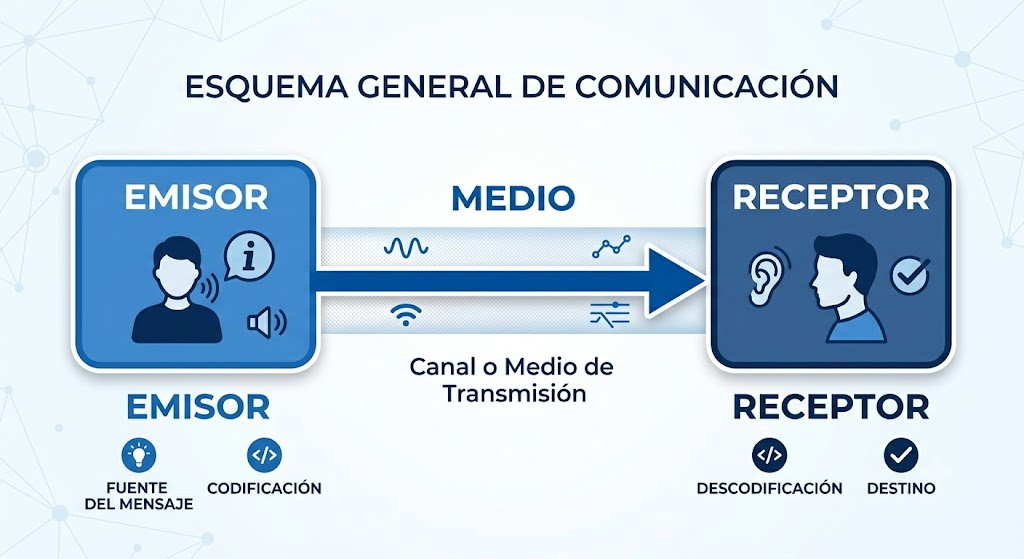
\includegraphics[width=0.8\textwidth]{assets/cap1/1.1.jpeg}
\caption{Modelo conceptual de cualquier comunicación: origen, medio y destino}
\label{fig:modelo-comunicacion}
\end{figure}

Hoy en día, la decisión más básica que enfrenta un diseñador de sistemas embebidos es: ¿transmito los datos en paralelo o en serie?


\section{Transmisión paralela vs. transmisión en serie}

\subsection{Transferencia en paralelo}

En una transmisión paralela, todos los bits de una palabra de datos se envían simultáneamente por múltiples líneas independientes. Por ejemplo, para transmitir un byte completo (8 bits), se necesitan 8 cables de datos, más las líneas de control y tierra.

\begin{definicion}
La \textbf{transferencia de datos en paralelo} es un método de comunicación en el que todos los bits de una palabra de datos se transmiten simultáneamente a través de múltiples canales físicos independientes.
\end{definicion}

Las ventajas parecen claras: es rápida, ya que un byte completo llega en un solo ciclo. Sin embargo, esta aparente ventaja desaparece cuando se analizan los problemas físicos:

\begin{itemize}
    \item \textbf{Coste hardware elevado}: cada bit requiere su propio conductor, conector y circuito de E/S.
    \item \textbf{Diafonía}: a alta velocidad, las señales eléctricas de un cable se acoplan a los adyacentes por efecto capacitivo e inductivo, generando ruido.
    \item \textbf{Sesgo de tiempo (skew)}: los cables no tienen exactamente la misma longitud ni impedancia, por lo que los bits llegan ligeramente desfasados. A velocidades altas, este desfase puede causar errores.
    \item \textbf{Limitación de distancia}: a frecuencias de decenas de Mb/s, los buses paralelos solo funcionan en trayectos de pocos centímetros. A Gb/s, apenas unos milímetros dentro de un chip.
\end{itemize}

\begin{figure}[H]
\centering
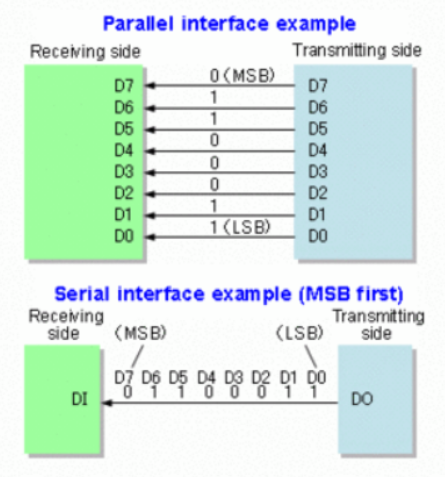
\includegraphics[width=0.8\textwidth]{assets/cap1/1.2.png}
\caption{Comparación visual: transmisión paralela (8 líneas) vs. transmisión en serie (1 línea)}
\label{fig:paralelo-vs-serie}
\end{figure}

\subsection{Transferencia en serie}

En una transmisión en serie, los bits se envían uno tras otro por una única línea de datos (más tierra). El byte completo tarda más tiempo en llegar, pero el hardware es mucho más sencillo.

\begin{definicion}[formal de transferencia en serie]
La \textbf{transferencia de datos en serie} es un método de comunicación en el que los bits de una palabra se transmiten secuencialmente, uno tras otro, a través de un único canal físico.
\end{definicion}

Las ventajas de la transmisión en serie son:
\begin{itemize}
    \item \textbf{Menor coste}: un solo cable de datos, conectores más pequeños y menos pines en los circuitos integrados.
    \item \textbf{Mayor inmunidad al ruido}: con técnicas de transmisión diferencial (ver sección \ref{sec:balanceado}), el ruido se cancela.
    \item \textbf{Distancias mayores}: algunas interfaces serie alcanzan cientos de metros (RS-485) o kilómetros (fibra óptica).
    \item \textbf{Velocidades elevadas}: aunque los bits llegan de uno en uno, las frecuencias de reloj pueden ser muy altas (Gb/s en USB, SATA, fibra óptica).
\end{itemize}

La principal desventaja es temporal: transmitir un byte en serie tarda más que en paralelo. Sin embargo, en la mayoría de aplicaciones industriales y de comunicaciones, esta diferencia es irrelevante frente a los beneficios de simplicidad y fiabilidad.

\begin{table}[htbp]
\centering
\small
\caption{Comparativa: transmisión paralela vs. en serie}
\begin{tabularx}{\textwidth}{@{}lXX@{}}
\toprule
\textbf{Característica} & \textbf{Paralelo} & \textbf{Serie} \\
\midrule
Número de líneas de datos & N (una por bit) & 1 \\
Velocidad por transferencia & Alta (1 byte/ciclo) & Más lenta (1 bit/ciclo) \\
Coste hardware & Elevado (muchos pines, cables) & Bajo (pocos pines, cables) \\
Diafonía & Problema grave a alta velocidad & Prácticamente nulo \\
Distancia máxima & Centímetros a metros & Metros a kilómetros \\
Aplicaciones típicas & Buses internos de PCB, RAM & USB, Ethernet, UART, SATA \\
\bottomrule
\end{tabularx}
\end{table}


\subsection{Principales interfaces de comunicación serie}

A continuación se resumen las interfaces serie más relevantes en el ámbito de la electrónica, la informática industrial y las redes de comunicaciones:

\begin{table}[H]
\centering
\footnotesize
\caption{Principales tipos de interfaces seriales}
\begin{tabularx}{\textwidth}{@{}>{\raggedright\arraybackslash}p{2.5cm}>{\raggedright\arraybackslash}X>{\raggedright\arraybackslash}p{3.5cm}@{}}
\toprule
\textbf{Interfaz} & \textbf{Descripción} & \textbf{Aplicación típica} \\
\midrule
SPI & Comunicación síncrona de alta velocidad. Maestro y múltiples esclavos. & Memoria flash, pantallas, tarjetas SD \\
I2C & Comunicación bidireccional con dos líneas (datos y reloj). & Sensores, EEPROM, displays \\
UART & Protocolo asíncrono básico, común en sistemas embebidos. & Debug, GPS, módems, Bluetooth \\
RS-232 / RS-422 / RS-485 & Estándares industriales. RS-232 en módems; RS-485 en automatización. & PLCs, módems, redes industriales \\
USB & Interfaz estándar moderna para periféricos de computadora. & Teclados, discos, cámaras \\
SATA & Conexión de discos duros internos. & SSD, HDD \\
CAN & Red para automoción y automatización industrial. & Automóviles, maquinaria, buses \\
1-Wire & Interfaz de bajo costo para pocos componentes. & Sensores de temperatura, iButton \\
\bottomrule
\end{tabularx}
\end{table}


\section{Tipos de codificación en comunicaciones serie}

Antes de que los bits viajen por el medio físico, deben convertirse en señales eléctricas (o luminosas) que el receptor pueda interpretar. El proceso de convertir un bit lógico (0 o 1) en una forma de onda física se denomina \textbf{codificación de línea}. La elección de la codificación afecta directamente a la inmunidad al ruido, la capacidad de recuperación de reloj y la eficiencia espectral del canal.

\subsection{NRZ (Non-Return-to-Zero)}

En la codificación NRZ, el nivel de tensión se mantiene constante durante todo el periodo de bit: un nivel alto representa un ``1'' y un nivel bajo representa un ``0''. Es el método más sencillo, pero presenta dos inconvenientes principales: no garantiza transiciones cuando se transmiten largas secuencias del mismo bit, lo que dificulta la recuperación de reloj, y tiene una componente continua (DC) que no es adecuada para algunos medios acoplados con transformador.

\begin{figure}[H]
\centering
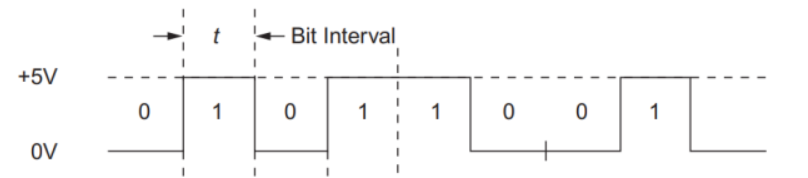
\includegraphics[width=0.8\textwidth]{assets/cap1/1.3.png}
\caption{Ejemplo de codificación NRZ para una secuencia de bits}
\label{fig:codificacion-nrz}
\end{figure}

\subsection{NRZ bipolar}

En la codificación NRZ bipolar, los bits ``1'' y ``0'' se representan mediante dos niveles de tensión de polaridad opuesta (por ejemplo, $+$V para ``1'' y $-$V para ``0''). A diferencia del NRZ unipolar, esta variante no presenta componente continua y mejora la inmunidad al ruido, ya que el receptor puede detectar la información midiendo la polaridad de la señal.

\begin{figure}[H]
\centering
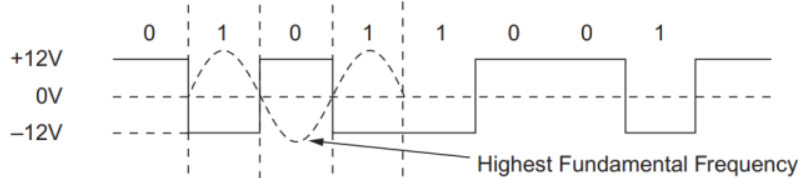
\includegraphics[width=0.8\textwidth]{assets/cap1/1.4.png}
\caption{Ejemplo de codificación NRZ bipolar}
\label{fig:codificacion-nrz-bipolar}
\end{figure}

\subsection{NRZ invertida (NRZ-I)}

En la codificación NRZ invertida (NRZ-I), la señal \textbf{no cambia} para un ``0'' y \textbf{invierte} su polaridad para un ``1''. De esta forma, una secuencia de unos produce transiciones continuas, mientras que una secuencia de ceros mantiene el nivel. NRZ-I se utiliza en interfaces como USB (junto con bit stuffing) para garantizar suficientes transiciones y permitir la recuperación de reloj.

\begin{figure}[H]
\centering
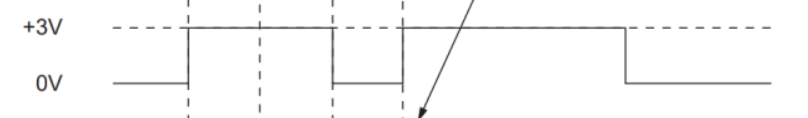
\includegraphics[width=0.8\textwidth]{assets/cap1/1.5.png}
\caption{Ejemplo de codificación NRZ invertida (NRZ-I)}
\label{fig:codificacion-nrzi}
\end{figure}

\subsection{RZ (Return-to-Zero)}

En RZ, la señal vuelve a cero (o al nivel de referencia) en la \textbf{mitad} del periodo de bit, independientemente del valor transmitido. Por ejemplo, en RZ unipolar, un ``1'' se representa como un pulso positivo seguido de un retorno a cero, mientras que un ``0'' se mantiene en nivel cero. Aunque simplifica la sincronización, consume más ancho de banda que NRZ.

\begin{figure}[H]
\centering
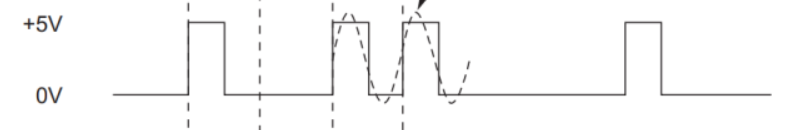
\includegraphics[width=0.8\textwidth]{assets/cap1/1.6.png}
\caption{Ejemplo de codificación RZ (Return-to-Zero)}
\label{fig:codificacion-rz}
\end{figure}

\subsection{RZ bipolar}

En la variante RZ bipolar, un ``1'' se representa como un pulso positivo seguido de retorno a cero, y un ``0'' como un pulso negativo seguido de retorno a cero. Requiere tres niveles de tensión (positivo, cero y negativo), lo que complica los circuitos, pero proporciona una referencia de nivel clara y permite detectar la pérdida de señal.

\begin{figure}[H]
\centering
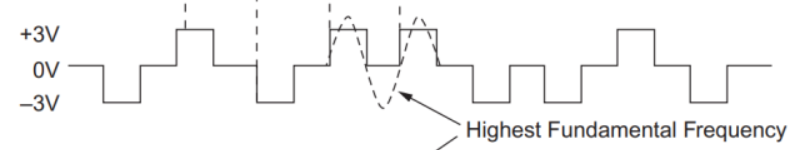
\includegraphics[width=0.8\textwidth]{assets/cap1/1.7.png}
\caption{Ejemplo de codificación RZ bipolar}
\label{fig:codificacion-rz-bipolar}
\end{figure}

\subsection{Manchester}

La codificación Manchester resuelve el problema de la recuperación de reloj generando \textbf{siempre una transición en el centro de cada bit}: una transición de bajo a alto representa un ``1'', y de alto a bajo representa un ``0''. Garantiza una transición por bit, lo que facilita enormemente la sincronización, pero duplica el ancho de banda necesario porque la frecuencia de la señal es el doble de la tasa de bits. Se empleó históricamente en Ethernet 10BASE-T.

\begin{figure}[H]
\centering
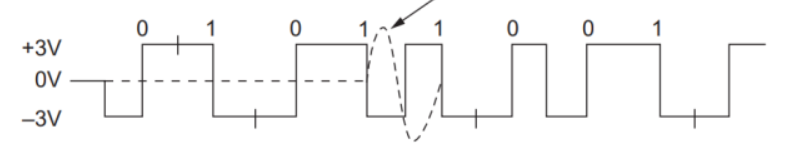
\includegraphics[width=0.8\textwidth]{assets/cap1/1.8.png}
\caption{Ejemplo de codificación Manchester}
\label{fig:codificacion-manchester}
\end{figure}

\begin{table}[htbp]
\centering
\small
\caption{Resumen comparativo de codificaciones de línea}
\begin{tabularx}{\textwidth}{@{}lXXX@{}}
\toprule
\textbf{Codificación} & \textbf{Transiciones} & \textbf{Componente DC} & \textbf{Uso típico} \\
\midrule
NRZ & No garantizadas & Sí & UART, SPI (interno) \\
NRZ bipolar & En cada bit (cambio de polaridad) & No & Telecomunicaciones \\
NRZ-I (invertida) & Sólo en unos (con bit stuffing) & Sí & USB \\
RZ (unipolar) & Garantizadas (retorno a cero) & Sí & Canales de fibra óptica antiguos \\
RZ bipolar & Garantizadas (tres niveles) & No & Telecomunicaciones, satélite \\
Manchester & Garantizadas (1/bit) & No & Ethernet 10BASE-T \\
\bottomrule
\end{tabularx}
\end{table}


\section{Conceptos fundamentales de las comunicaciones serie}
\label{sec:fundamentos}

\subsection{Topologías de conexión}

La topología describe cómo se conectan físicamente los nodos de una red:

\begin{itemize}
    \item \textbf{Punto a punto (peer-to-peer)}: la conexión más simple, con solo dos nodos. Ejemplo: un PC conectado a una impresora, o un microcontrolador a un sensor.
    \item \textbf{Bus}: todos los nodos comparten un mismo medio de transmisión. Ejemplo: RS-485, CAN bus.
    \item \textbf{Estrella}: todos los nodos se conectan a un nodo central. Ejemplo: Ethernet con switch, USB con hub.
    \item \textbf{Anillo}: cada nodo se conecta a dos vecinos, formando un círculo. Ejemplo: redes industriales antiguas, anillos ópticos.
\end{itemize}

\begin{figure}[H]
\centering
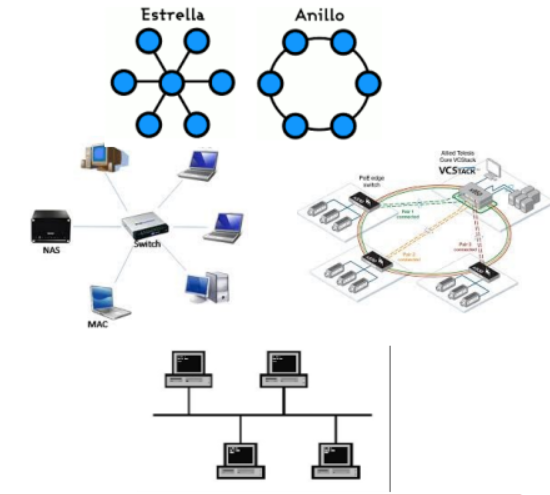
\includegraphics[width=0.8\textwidth]{assets/cap1/1.9.png}
\caption{Las cuatro topologías básicas en comunicaciones serie}
\label{fig:topologias}
\end{figure}

\subsection{Configuraciones balanceadas vs. no balanceadas}
\label{sec:balanceado}

Esta distinción es fundamental para entender la inmunidad al ruido de una comunicación.

\subsubsection{Conexión no balanceada (single-ended)}

En una conexión no balanceada, la señal se transmite por un único conductor y se toma como referencia la tierra (GND). El voltaje de la señal se mide respecto a tierra.

\begin{definicion}[formal de conexión no balanceada]
Una conexión \textbf{no balanceada} (o desbalanceada) es aquella en la que el voltaje de señal se referencia a un punto de tierra común, utilizando un único conductor para transportar la información.
\end{definicion}

Es sencilla y económica, pero tiene un problema grave: cualquier ruido inducido en el cable o diferencia de potencial entre las tierras de los dos dispositivos se suma directamente a la señal, pudiendo causar errores.

\subsubsection{Conexión balanceada (diferencial)}

En una conexión balanceada, la señal se transmite por dos conductores, ninguno de los cuales está conectado a tierra. Los voltajes en ambos conductores son de polaridad opuesta respecto a tierra. El receptor no mide el voltaje respecto a tierra, sino la \textbf{diferencia} entre ambos conductores.

\begin{definicion}[formal de conexión balanceada]
Una conexión \textbf{balanceada} (o diferencial) es aquella en la que la señal se transmite mediante dos conductores con voltajes de polaridad opuesta, y el receptor recupera la información calculando la diferencia entre ambos voltajes.
\end{definicion}

\textbf{¿Por qué cancela el ruido?} Si un ruido externo se acopla a la línea, afecta por igual a los dos conductores. Como el receptor resta los voltajes, la componente de ruido común ($V_{ruido} - V_{ruido} = 0$) desaparece. Esto se conoce como \textbf{rechazo al modo común (CMRR)}.

\begin{figure}[H]
\centering
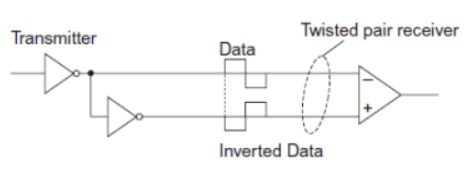
\includegraphics[width=0.8\textwidth]{assets/cap1/1.10.png}
\caption{Cancelación del ruido en una conexión balanceada (diferencial)}
\label{fig:balanceada}
\end{figure}

\subsection{Medios de transmisión físicos}

Los datos en serie pueden viajar por diferentes medios. Los más comunes son:

\subsubsection{Líneas en placa de circuito impreso (PCB)}

Son las trazas de cobre que conectan chips dentro de una misma placa. Son cortas (centímetros) y pueden ser desbalanceadas (traza + tierra) o balanceadas (dos trazas paralelas). Su uso se limita a comunicaciones internas de alta velocidad entre circuitos integrados vecinos.

\subsubsection{Cable coaxial}

Un conductor central rodeado por una malla metálica (blindaje) y una cubierta exterior. Es una línea desbalanceada con impedancia característica típica de $50\,\Omega$. Aunque la atenuación es considerable, puede transportar señales de varios Gb/s en distancias cortas. Hoy se usa principalmente en RF y en algunas redes de comunicaciones.

\begin{figure}[H]
\centering
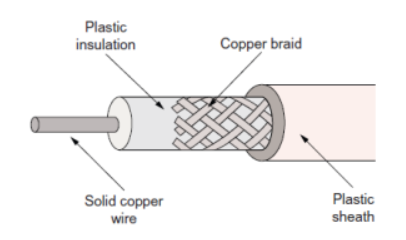
\includegraphics[width=0.8\textwidth]{assets/cap1/1.11.png}
\caption{Ejemplo de cable coaxial}
\label{fig:cable-coaxial}
\end{figure}

\subsubsection{Par trenzado (UTP/STP)}

Dos cables aislados retorcidos entre sí, sin blindaje (UTP) o con blindaje (STP). Es el medio más utilizado en redes modernas:
\begin{itemize}
    \item El retorcido reduce la diafonía entre pares adyacentes.
    \item El blindaje (en STP) protege en entornos industriales ruidosos.
    \item Ejemplos: cableado telefónico, Ethernet CAT5/CAT6.
\end{itemize}

\begin{figure}[H]
\centering
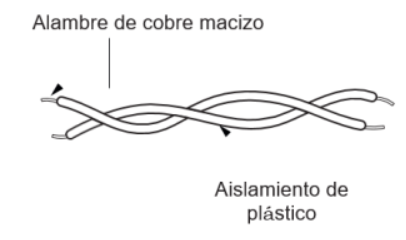
\includegraphics[width=0.8\textwidth]{assets/cap1/1.12.png}
\caption{Ejemplo de par trenzado (UTP/STP)}
\label{fig:par-trenzado}
\end{figure}

\subsubsection{Fibra óptica}

Un núcleo de vidrio o plástico rodeado de revestimiento y cubierta. Los datos se convierten en pulsos de luz infrarroja generados por LEDs o láseres. En el receptor, un fotodiodo (PIN o avalancha) convierte la luz de nuevo en señal eléctrica.

Sus ventajas son excepcionales:
\begin{itemize}
    \item Velocidades superiores a 100\,Gb/s.
    \item Inmunidad total al ruido eléctrico y a la diafonía.
    \item Distancias de kilómetros sin regeneración.
\end{itemize}

\begin{figure}[H]
\centering
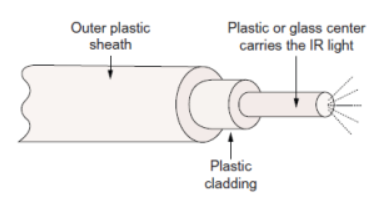
\includegraphics[width=0.8\textwidth]{assets/cap1/1.13.png}
\caption{Ejemplo de fibra óptica}
\label{fig:fibra-optica}
\end{figure}


\section{El reloj: cómo se sincronizan emisor y receptor}
\label{sec:reloj}

En cualquier comunicación digital, el receptor debe saber \textbf{cuándo} leer cada bit. Si muestrea demasiado pronto o demasiado tarde, leerá un valor incorrecto. La sincronización se resuelve mediante una señal de reloj. En comunicaciones serie existen tres estrategias fundamentales.

\subsection{Transmisión asíncrona: relojes independientes}

Cada dispositivo tiene su propio reloj interno. Los relojes no están sincronizados, pero deben coincidir aproximadamente en frecuencia. Para que el receptor sepa cuándo empieza un nuevo dato, el transmisor añade un \textbf{bit de inicio} (start bit) antes de los datos propiamente dichos. Al detectar esta transición, el receptor recalibra su muestreo para el byte siguiente.

\begin{figure}[H]
\centering
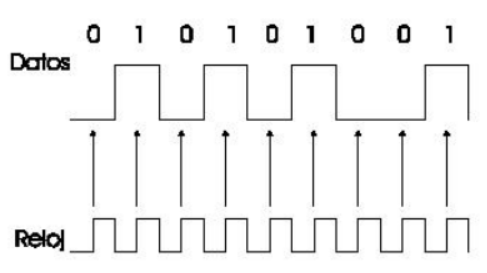
\includegraphics[width=0.8\textwidth]{assets/cap1/1.14.png}
\caption{Formato típico de una transmisión asíncrona byte a byte (ejemplo UART)}
\label{fig:trama-asincrona}
\end{figure}

\textbf{Ventaja}: solo se necesita una línea de datos (más tierra). 
\textbf{Limitación}: las frecuencias de reloj deben ser muy similares, y se desperdicia algo de tiempo en los bits de sincronización de cada byte.

\subsection{Transmisión síncrona: reloj en línea separada}

El transmisor envía una señal de reloj por un cable adicional, junto con la línea de datos. El receptor muestrea los datos exactamente en los flancos de este reloj externo.

\textbf{Ventaja}: sincronización perfecta, sin margen de error por desajuste de relojes.
\textbf{Desventaja}: requiere una línea adicional (dos líneas de señal + tierra), lo que encarece el cableado.

\subsection{Recuperación de reloj desde los datos (CDR)}

En las comunicaciones más rápidas, no hay línea de reloj separada ni bits de inicio/parada. El receptor extrae el reloj directamente de las transiciones de la propia señal de datos. Para que esto funcione, los datos deben codificarse de forma que haya suficientes transiciones (0→1 y 1→0), evitando secuencias largas del mismo nivel.

\begin{definicion}[formal de CDR]
La técnica de \textbf{reloj y recuperación de datos (CDR, Clock and Data Recovery)} consiste en reconstruir la señal de reloj a partir de las transiciones de la propia señal de datos recibida, permitiendo la sincronización sin necesidad de una línea de reloj separada.
\end{definicion}

Este método se usa en interfaces de alta velocidad como USB 3.0, SATA, PCIe y Ethernet de fibra óptica.

\begin{table}[htbp]
\centering
\small
\caption{Los tres métodos de sincronización en comunicaciones serie}
\begin{tabularx}{\textwidth}{@{}lXX@{}}
\toprule
\textbf{Método} & \textbf{Característica} & \textbf{Ejemplo} \\
\midrule
Asíncrona & Relojes independientes, bits de inicio/parada & UART, RS-232 \\
Síncrona (reloj separado) & Línea de reloj adicional, perfecta sincronización & SPI, I2C \\
CDR & Reloj extraído de los datos, codificación especial & USB 3.0, SATA, Ethernet \\
\bottomrule
\end{tabularx}
\end{table}


\section{Formatos de trama y protocolos}

Un \textbf{protocolo} es el conjunto de reglas que definen cómo se comunican dos dispositivos: el formato de los datos, el orden de los bits, la detección de errores, el control de flujo, etc.

La mayoría de los datos se envían en bloques estructurados llamados \textbf{tramas} o \textbf{frames}. Aunque cada protocolo tiene su propio formato, la estructura general sigue un patrón común:

\begin{enumerate}
    \item \textbf{Delimitador de inicio}: una secuencia especial de bits que indica ``aquí empieza una trama''.
    \item \textbf{Dirección}: identifica el nodo destino (y a veces el origen).
    \item \textbf{Datos}: el contenido propiamente dicho, normalmente un bloque de bytes.
    \item \textbf{Código de control de errores}: un valor calculado a partir de los datos (paridad, CRC, BCC) para detectar o corregir errores.
    \item \textbf{Delimitador de fin}: señala el final de la trama.
\end{enumerate}

\begin{figure}[H]
\centering
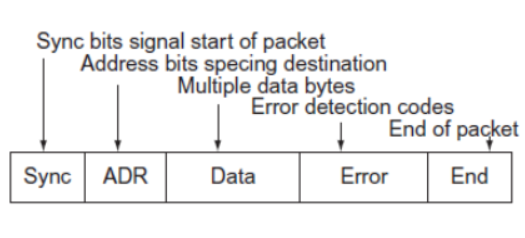
\includegraphics[width=0.8\textwidth]{assets/cap1/1.15.png}
\caption{Estructura genérica de una trama de datos en comunicaciones serie}
\label{fig:trama-generica}
\end{figure}

\subsection{Transmisión asíncrona vs. síncrona de tramas}

\begin{itemize}
    \item \textbf{Asíncrona}: cada byte se envía de forma independiente con sus propios bits de inicio y parada. No hay una estructura de trama compleja; se transmiten bytes sueltos.
    \item \textbf{Síncrona}: los datos se agrupan en tramas largas. No hay bits de inicio/parada por cada byte; en su lugar, la trama comienza con un delimitador especial y el receptor usa CDR o una línea de reloj para muestrear continuamente.
\end{itemize}


\section{Detección y corrección de errores}

El ruido electromagnético, las interferencias y las imperfecciones del medio pueden alterar los bits durante la transmisión. Por eso, los protocolos serie incorporan mecanismos para detectar o incluso corregir errores.

\subsection{Bit de paridad}

Es el método más sencillo. Consiste en añadir un bit extra a cada byte transmitido, de forma que el número total de bits a 1 sea par (paridad par) o impar (paridad impar).

\begin{definicion}[formal del bit de paridad]
El \textbf{bit de paridad} es un bit adicional que se añade a una palabra de datos para que el número total de bits con valor 1 sea par (paridad par) o impar (paridad impar). El receptor recuenta los bits y compara con el bit de paridad recibido; si hay discrepancia, se detecta un error.
\end{definicion}

\textbf{Limitación}: solo detecta errores cuando cambia un número impar de bits. Si dos bits se invierten simultáneamente, la paridad no lo detecta. Además, no indica qué bit está mal, solo que ha ocurrido un error.

\subsection{Código de verificación de bloques (BCC / BCS)}

En lugar de verificar byte a byte, se puede calcular un código de verificación para un bloque completo de datos. Un método sencillo es el \textbf{BCC (Block Check Character)}: se suman (o se hace XOR) todos los bytes del bloque, y el resultado final se envía como un carácter de verificación al final de la trama. El receptor repite el cálculo y compara.

Este método permite detectar errores en múltiples bits del bloque, pero no identificar la posición exacta del error.

\subsection{Verificación de redundancia cíclica (CRC)}

El CRC es el método más robusto de detección de errores en comunicaciones serie industriales. Se trata los bits de datos como una secuencia binaria y se divide por un polinomio generador predefinido mediante aritmética modular. El resto de esta división (el CRC) se adjunta a la trama y se verifica en el receptor.

El CRC detecta eficazmente las \textbf{ráfagas de errores} (varios bits consecutivos alterados), siempre que la longitud de la ráfaga no supere el grado del polinomio generador.

\begin{table}[htbp]
\centering
\small
\caption{Comparativa de métodos de detección de errores}
\begin{tabularx}{\textwidth}{@{}lXXX@{}}
\toprule
\textbf{Método} & \textbf{Complejidad} & \textbf{Eficacia} & \textbf{Uso típico} \\
\midrule
Bit de paridad & Muy baja & Detecta 1 bit impar & UART, RS-232 \\
BCC/BCS & Baja & Detecta errores simples & Protocolos antiguos \\
CRC & Media & Detecta ráfagas de errores & Ethernet, CAN, USB, industrial \\
\bottomrule
\end{tabularx}
\end{table}


\subsection{Corrección de errores de reenvío (FEC)}

Además de detectar errores, algunos protocolos de comunicación serie son capaces de \textbf{corregirlos} sin necesidad de retransmisión. La técnica se conoce como \textbf{Forward Error Correction (FEC)} o corrección de errores de reenvío.

Los métodos FEC añaden información redundante calculada a partir de los datos originales. Si la señal recibida se deteriora por ruido o interferencias, el receptor utiliza esa redundancia para reconstruir los bits erróneos. Esto mejora la fiabilidad de la transmisión y reduce la tasa de errores de bits (BER).

Una ventaja notable de los sistemas FEC es que, en presencia de ruido, actúan como si el sistema produjera \textbf{ganancia de codificación}. Esta ganancia compensa el ruido en el canal y permite alcanzar velocidades de datos más altas sin aumentar la potencia de transmisión. Por ello, el FEC es fundamental en interfaces seriales de alta velocidad, comunicaciones por satélite y sistemas de almacenamiento masivo.




\section{Métodos de acceso al medio}

Cuando más de dos dispositivos comparten un mismo medio de transmisión, es necesario establecer un mecanismo que determine quién puede transmitir y cuándo. Estos mecanismos se denominan \textbf{métodos de acceso al medio} y son la base de cualquier red multipunto o bus compartido.

\subsection{Maestro--Esclavo}

En un sistema de acceso maestro--esclavo, un único dispositivo \textbf{maestro} controla dos o más dispositivos \textbf{esclavos}. El maestro decide qué esclavo debe transmitir o recibir en cada momento, evitando colisiones en el medio compartido. Los protocolos de interfaz utilizan comandos específicos para instruir a los esclavos, y todas las operaciones están determinadas por el maestro.

Una técnica común es el \textbf{sondeo} (polling): el maestro consulta a cada esclavo en secuencia, enviando o recibiendo datos según sea necesario. Si un esclavo no tiene información, responde con una indicación de ``no hay datos'' y el maestro pasa al siguiente. Este método es sencillo, determinista y ampliamente utilizado en buses industriales como SPI y I2C.

\begin{figure}[H]
\centering
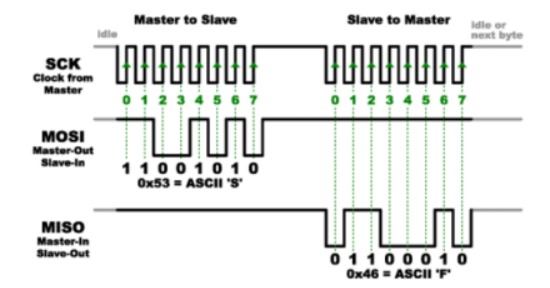
\includegraphics[width=0.8\textwidth]{assets/cap1/1.16.png}
\caption{Topología maestro--esclavo en un bus compartido}
\label{fig:maestro-esclavo}
\end{figure}

\subsection{CSMA (Carrier Sense Multiple Access)}

El \textbf{acceso múltiple por detección de portadora (CSMA)} es un sistema en el que todos los nodos de un bus ``escuchan'' el medio antes de transmitir. Si detectan que ya hay datos en tránsito (un ``portador'' presente), esperan para evitar colisiones.

La mayoría de los sistemas CSMA incorporan también \textbf{detección de colisiones (CD)}. Si dos dispositivos transmiten simultáneamente, sus señales se mezclan y generan errores. CSMA/CD detecta la colisión, hace que ambos nodos dejen de transmitir y esperen un tiempo aleatorio antes de reintentarlo. Aunque este método maneja automáticamente la contención, la competencia por el bus reduce el rendimiento global y aumenta la latencia, especialmente cuando hay muchos nodos activos.

\begin{figure}[H]
\centering
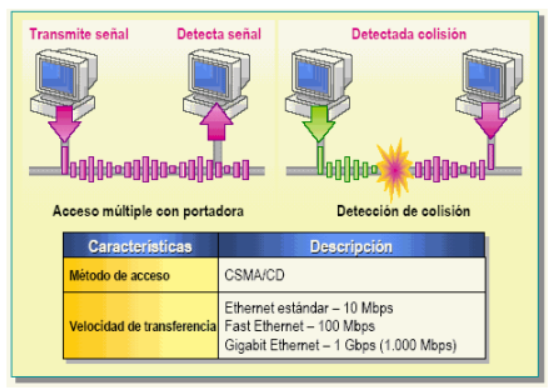
\includegraphics[width=0.8\textwidth]{assets/cap1/1.17.png}
\caption{Ejemplo de CSMA/CD con detección de colisión y retransmisión}
\label{fig:csma-cd}
\end{figure}

\subsection{TDMA (Time Division Multiple Access)}

El \textbf{acceso múltiple por división de tiempo (TDMA)} asigna a cada nodo una \textbf{franja horaria} (time slot) dentro de un ciclo periódico. El sistema define una unidad de tiempo para un ciclo completo y la divide en intervalos, uno para cada nodo del medio compartido. Cuando un dispositivo necesita transmitir, espera su intervalo asignado y envía los datos durante ese tiempo.

Las franjas horarias suelen ser de una palabra o un byte, aunque pueden ser más largas según el protocolo. Aunque la velocidad de transmisión instantánea de cada nodo se ve limitada por este método, en la mayoría de sistemas industriales la velocidad global es tan alta que el tiempo añadido no supone una desventaja significativa. TDMA es muy común en redes inalámbricas, sistemas GSM y buses industriales deterministas.

\begin{figure}[H]
\centering
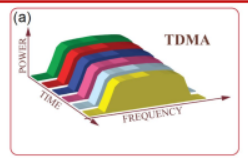
\includegraphics[width=0.8\textwidth]{assets/cap1/1.18.png}
\caption{Ejemplo de ciclo TDMA con cuatro nodos}
\label{fig:tdma}
\end{figure}

\subsection{Dúplex (Duplexing)}

El término \textbf{dúplex} se refiere a la direccionalidad de las comunicaciones entre dos dispositivos:

\begin{itemize}
    \item \textbf{Simplex}: comunicación unidireccional. Solo un dispositivo transmite y el otro recibe; no hay respuesta. Ejemplo: un sensor que envía lecturas continuamente a un display.
    \item \textbf{Semidúplex (half-duplex)}: ambos dispositivos pueden transmitir y recibir, pero \textbf{no simultáneamente}. Comparten un único canal y alternan turnos. Ejemplo: walkie-talkies, RS-485 en modo semidúplex.
    \item \textbf{Dúplex completo (full-duplex)}: transmisión y recepción \textbf{simultáneas}. En sistemas cableados se requieren dos canales físicos (uno para cada dirección). Ejemplo: UART, RS-232, Ethernet.
\end{itemize}

En sistemas inalámbricos o con un solo par de conductores, el dúplex completo se puede lograr mediante técnicas de multiplexación como TDMA, donde los slots de transmisión y recepción se alternan a gran velocidad, dando la apariencia de comunicación simultánea.


\section{El estándar RS-232: comunicación serie industrial}
\label{sec:rs232}

\subsection{¿Qué es RS-232?}

El estándar \textbf{RS-232} (Recommended Standard 232) es una de las interfaces de comunicación serie más antiguas y duraderas de la industria electrónica. Aunque hoy coexisten con USB, Wi-Fi y Ethernet, el RS-232 sigue siendo ampliamente utilizado en entornos industriales, de automatización y de pruebas de equipos.

\begin{definicion}[formal de RS-232]
La interfaz \textbf{RS-232} es un estándar de comunicación serie asíncrona que define la transmisión de datos binarios entre un equipo \textbf{DTE} (Data Terminal Equipment, equipo terminal de datos) y un equipo \textbf{DCE} (Data Circuit-terminating Equipment, equipo de comunicación de datos). Especifica las características eléctricas, mecánicas y funcionales de la conexión.
\end{definicion}

\textbf{Ejemplos clásicos de dispositivos}:
\begin{itemize}
    \item \textbf{DTE}: ordenadores personales, terminales, PLCs, microcontroladores como el ESP32.
    \item \textbf{DCE}: módems, convertidores de interfaz, dispositivos de medición.
\end{itemize}

\begin{figure}[H]
\centering
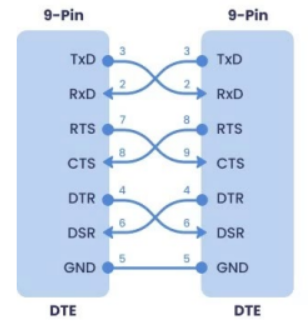
\includegraphics[width=0.8\textwidth]{assets/cap1/1.19.png}
\caption{Modelo DTE-DCE en una comunicación RS-232}
\label{fig:dte-dce}
\end{figure}

\subsection{Niveles de tensión: la gran diferencia con UART/TTL}

La diferencia más importante entre UART (a nivel TTL) y RS-232 es el \textbf{nivel de tensión}:

\begin{itemize}
    \item \textbf{UART/TTL} (0V / 3.3V o 5V): señales de bajo voltaje, idóneas para comunicaciones internas en PCB o cortas distancias.
    \item \textbf{RS-232} ($\pm$3V a $\pm$15V, típicamente $\pm$12V): señales de mayor amplitud, mucho más inmunes al ruido electromagnético y capaces de recorrer distancias mayores (hasta 15 metros a velocidades moderadas).
\end{itemize}

\begin{table}[htbp]
\centering
\small
\caption{Comparativa de niveles de tensión: TTL vs. RS-232}
\begin{tabular}{@{}lcc@{}}
\toprule
\textbf{Parámetro} & \textbf{UART/TTL} & \textbf{RS-232} \\
\midrule
Nivel lógico 0 (espacio) & 0V & +3V a +15V \\
Nivel lógico 1 (marca) & 3.3V o 5V & $-$3V a $-$15V \\
Inversión de señal & No & Sí (0 $\rightarrow$ +V, 1 $\rightarrow$ $-$V) \\
Distancia máxima & $<$1 metro & Hasta 15 metros \\
Inmunidad al ruido & Baja & Alta \\
\bottomrule
\end{tabular}
\end{table}

\textbf{¡Atención!} En RS-232, los niveles están \textbf{invertidos} respecto a TTL: un ``0'' lógico se transmite como voltaje positivo, y un ``1'' lógico como voltaje negativo. Esto es crucial al interpretar señales en un osciloscopio.

\subsection{Conectores y pines}

RS-232 utiliza conectores tipo D-sub:
\begin{itemize}
    \item \textbf{DB-9}: 9 pines, el más común hoy en día.
    \item \textbf{DB-25}: 25 pines, versión original del estándar.
\end{itemize}

De los 9 pines del DB-9, solo \textbf{tres} son imprescindibles para una comunicación básica:
\begin{enumerate}
    \item \textbf{TXD (Transmit Data, pin 3)}: salida de datos desde el DTE.
    \item \textbf{RXD (Receive Data, pin 2)}: entrada de datos al DTE.
    \item \textbf{GND (Signal Ground, pin 5)}: referencia de tierra común.
\end{enumerate}

Los pines restantes se usan para \textbf{control de flujo por hardware} (RTS, CTS, DTR, DSR, DCD, RI), aunque en muchas aplicaciones modernas se omiten.

\begin{figure}[H]
\centering
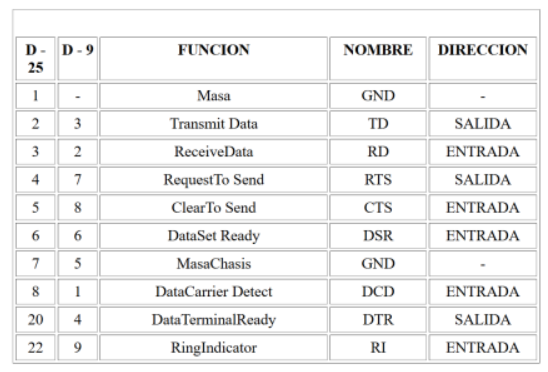
\includegraphics[width=0.8\textwidth]{assets/cap1/1.20.png}
\caption{Distribución de pines en un conector DB-9 para RS-232}
\label{fig:db9-pines}
\end{figure}

\subsection{Velocidad de subida y limitaciones}

El estándar RS-232 especifica una \textbf{velocidad de subida (slew rate)} máxima de $30\,$V/$\mu$s. Esta limitación intencionada evita que las transiciones rápidas generen interferencias electromagnéticas en señales adyacentes. Como consecuencia, la velocidad máxima de datos está limitada a aproximadamente \textbf{115.2 kb/s} (aunque en la práctica moderna se alcanzan 230.4 kb/s con cables cortos).

\subsection{Ventajas del RS-232 frente a otros protocolos}

\begin{itemize}
    \item \textbf{Mayor resistencia al ruido}: los voltajes de $\pm$12V son mucho más difíciles de alterar por interferencias que los 3.3V de TTL.
    \item \textbf{Distancias más largas}: hasta 15 metros frente a menos de 1 metro en TTL.
    \item \textbf{Compatibilidad universal}: existe hardware de conversión (TTL$\rightarrow$RS-232) muy económico y estandarizado.
    \item \textbf{Simplicidad de cableado}: solo dos hilos de datos + tierra para una comunicación básica.
\end{itemize}

\textbf{Limitaciones}: solo permite comunicación \textbf{punto a punto} (un DTE y un DCE), no es adecuado para redes multipunto. Para ello existen RS-485 y CAN bus.



\section{El protocolo USB: bus serie moderno}
\label{sec:usb}

\subsection{Introducción}

El \textbf{USB (Universal Serial Bus)} es el estándar de comunicación serie más extendido en la actualidad para la interconexión de periféricos con ordenadores y sistemas embebidos. Fue diseñado para sustituir a las interfaces antiguas (como RS-232, puerto paralelo y PS/2) con un único conector versátil, capaz de transmitir datos y alimentar el dispositivo al mismo tiempo.

\subsection{Características principales}

Las principales características del bus USB son:
\begin{itemize}
    \item \textbf{Topología punto a punto}: cada segmento conecta un host (o hub) con un único periférico o hub descendente.
    \item \textbf{Arquitectura maestro--esclavo}: el host (generalmente un PC) es el único maestro que inicia todas las comunicaciones; los periféricos responden únicamente cuando son interrogados.
    \item \textbf{Hasta 127 dispositivos}: mediante el uso de hubs en cascada, un único host puede gestionar hasta 127 periféricos simultáneamente.
    \item \textbf{Plug and Play}: los dispositivos pueden conectarse y desconectarse en caliente sin necesidad de apagar el equipo.
    \item \textbf{Alimentación integrada}: el cable proporciona una tensión nominal de 5\,V, lo que permite alimentar periféricos de bajo consumo directamente desde el bus.
    \item \textbf{Velocidades escalables}: desde 1.5\,Mb/s (Low Speed) hasta 20\,Gb/s (USB4) en sus versiones más recientes.
\end{itemize}

\subsection{Interfaz física y niveles eléctricos}

El cable USB estándar dispone de \textbf{cuatro hilos}:
\begin{enumerate}
    \item \textbf{VBUS} (+5\,V, rojo): alimentación para el periférico.
    \item \textbf{D--} (blanco): línea de datos diferencial negativa.
    \item \textbf{D+} (verde): línea de datos diferencial positiva.
    \item \textbf{GND} (negro): referencia de tierra común.
\end{enumerate}

La señal de datos se transmite por un \textbf{par trenzado diferencial} (D+ y D--) con una impedancia característica de 90\,$\Omega$. La sensibilidad del receptor es de al menos 200\,mV y debe soportar un alto factor de rechazo de modo común. La velocidad de transferencia puede ser de 1.5\,Mb/s, 12\,Mb/s, 480\,Mb/s, 5\,Gb/s, 10\,Gb/s o 20\,Gb/s, dependiendo de la versión del estándar.

\begin{figure}[H]
\centering
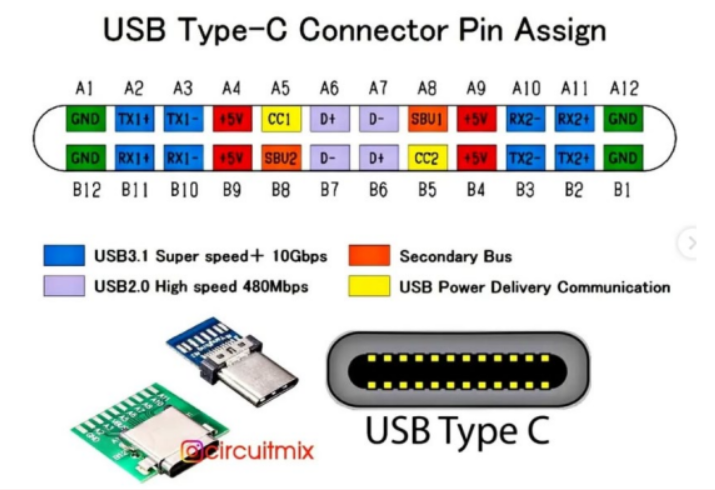
\includegraphics[width=0.8\textwidth]{assets/cap1/1.21.png}
\caption{Conector USB estándar y asignación de pines}
\label{fig:usb-pines}
\end{figure}

\subsection{Codificación y sincronización}

En USB, el reloj no se transmite por una línea separada, sino que se \textbf{recupera de los datos} mediante codificación NRZI. Para garantizar que haya suficientes transiciones y mantener la sincronización, el transmisor inserta \textbf{bits de relleno (bit stuffing)} cada vez que detecta seis unos consecutivos. Además, cada paquete comienza con un campo de sincronismo (SYNC) que permite al receptor ajustar su reloj interno.

\subsection{Terminología USB}

A continuación se definen los términos fundamentales que describen los elementos y roles de una arquitectura USB:

\begin{itemize}
    \item \textbf{Host.} Dispositivo maestro que inicia la comunicación (generalmente la computadora).
    \item \textbf{Hub.} Dispositivo que contiene uno o más conectores o conexiones internas hacia otros dispositivos USB, el cual habilita la comunicación entre el host y diversos dispositivos. Cada conector representa un puerto USB.
    \item \textbf{Dispositivo compuesto.} Es aquel dispositivo con múltiples interfaces independientes. Cada una tiene una dirección sobre el bus, pero cada interfaz puede tener un diferente driver de dispositivo en el host.
    \item \textbf{Puerto USB.} Cada host soporta solo un bus; cada conector en el bus representa un puerto USB. Por lo tanto, sobre el bus puede haber varios conectores, pero solo existe una ruta y solo un dispositivo puede transmitir información a un tiempo.
    \item \textbf{Driver.} Es un programa que habilita las aplicaciones para poder comunicarse con el dispositivo. Cada dispositivo sobre el bus debe tener un driver; algunos periféricos utilizan los drivers que trae el sistema operativo.
    \item \textbf{Puntos terminales (Endpoints).} Es una localidad específica dentro del dispositivo. El endpoint es un \textit{buffer} que almacena múltiples bytes, típicamente es un bloque de la memoria de datos o un registro dentro del microcontrolador. Todos los dispositivos deben soportar el punto terminal 0. Este punto terminal es el que recibe todo el control y las peticiones de estado durante la enumeración cuando el dispositivo está sobre el bus.
\end{itemize}

\begin{table}[htbp]
\centering
\small
\caption{Comparativa entre RS-232 y USB}
\begin{tabularx}{\textwidth}{@{}lXX@{}}
\toprule
\textbf{Característica} & \textbf{RS-232} & \textbf{USB} \\
\midrule
Modo de acceso & Punto a punto & Maestro--esclavo (host) \\
Balanceada & No (single-ended) & Sí (diferencial) \\
Velocidad máxima & 115.2\,kb/s & Hasta 20\,Gb/s (USB4) \\
Alimentación del bus & No & Sí (5\,V, hasta 500\,mA) \\
Conectores & DB-9, DB-25 & Tipo A, Tipo C, Micro-USB \\
Hot-plug & No & Sí \\
Número de dispositivos & 1 (P2P) & Hasta 127 (con hubs) \\
\bottomrule
\end{tabularx}
\end{table}


\section{Práctica 1: Comunicación UART con ESP32-S3}
\label{sec:practica1}

\subsection{Objetivos}

La Práctica 1 tiene como objetivos:
\begin{enumerate}
    \item Aprender a enviar y recibir datos mediante UART en modo asíncrono.
    \item Configurar el periférico UART de un microcontrolador (ESP32-S3) mediante su API.
    \item Examinar la señal UART física con un osciloscopio para comprender el formato de trama.
    \item Implementar una comunicación bidireccional entre un PC y un microcontrolador.
\end{enumerate}

\subsection{Material utilizado}

\begin{itemize}
    \item \textbf{Hardware}: PC, placa de desarrollo ESP32-S3-DevKitC-1, cable USB a TTL, osciloscopio.
    \item \textbf{Software}: Arduino IDE, Python (pyserial), drivers USB-UART.
\end{itemize}


\subsection{Marco teórico: protocolo UART}

\label{sec:uart}

Llegamos al protocolo protagonista de esta unidad y de la Práctica 1. El \textbf{UART} (Universal Asynchronous Receiver-Transmitter) es el protocolo de comunicación serie asíncrona más utilizado en electrónica digital y sistemas embebidos.

\subsubsection{Descripción del protocolo UART}

\begin{definicion}[formal de UART]
Un \textbf{UART (Universal Asynchronous Receiver-Transmitter)} es un circuito de hardware que implementa una comunicación serie asíncrona punto a punto, full-duplex, utilizando dos líneas de datos (TX y RX) y un nivel de tensión común de referencia (GND).
\end{definicion}

\textbf{Características principales}:
\begin{itemize}
    \item \textbf{Asíncrono}: no requiere línea de reloj compartida. La sincronización se logra mediante bits de inicio y parada.
    \item \textbf{Full-duplex}: ambos dispositivos pueden transmitir y recibir simultáneamente.
    \item \textbf{Punto a punto}: conecta exactamente dos dispositivos.
    \item \textbf{Pines mínimos}: TX (transmisión), RX (recepción) y GND (tierra común).
    \item \textbf{Niveles TTL}: típicamente 0V (lógica 0) y 3.3V o 5V (lógica 1). No confundir con RS-232, que usa voltajes mucho más altos ($\pm$12V).
\end{itemize}

\begin{figure}[H]
\centering
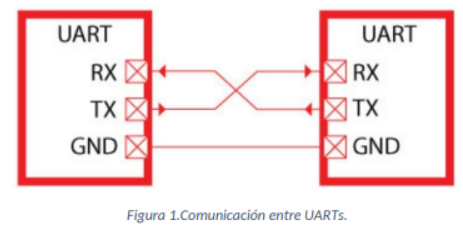
\includegraphics[width=0.8\textwidth]{assets/cap1/1.22.png}
\caption{Conexión cruzada entre dos dispositivos UART: TX de A con RX de B, y viceversa}
\label{fig:conexion-uart}
\end{figure}

\subsubsection{Formato de la trama UART}

La transmisión de un byte mediante UART sigue un formato estricto:

\begin{enumerate}
    \item \textbf{Estado de reposo (idle)}: la línea se mantiene a nivel alto (1) cuando no hay transmisión.
    \item \textbf{Bit de inicio (START)}: una transición a nivel bajo (0) durante un tiempo de bit. Indica al receptor que comienza un nuevo byte.
    \item \textbf{Bits de datos}: 5, 6, 7 u 8 bits (normalmente 8) que representan el carácter. El bit menos significativo (LSB) se envía primero.
    \item \textbf{Bit de paridad} (opcional): paridad par (E), impar (O), o sin paridad (N).
    \item \textbf{Bit(es) de parada (STOP)}: nivel alto (1) durante 0.5, 1, 1.5 o 2 tiempos de bit. Marca el final del byte.
\end{enumerate}

\begin{figure}[H]
\centering
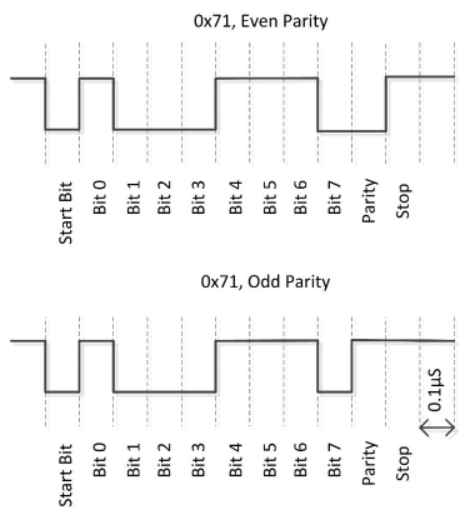
\includegraphics[width=0.8\textwidth]{assets/cap1/1.23.png}
\caption{Formato de trama UART para la configuración 8N1 (8 bits, sin paridad, 1 bit de parada)}
\label{fig:trama-uart}
\end{figure}

\subsubsection{Configuración de una comunicación UART}

Una comunicación UART se especifica mediante una cadena de parámetros:

\begin{center}
\textbf{\texttt{<velocidad> <bits de datos><paridad><bits de parada>}}
\end{center}

Ejemplos comunes:
\begin{itemize}
    \item \textbf{9600 8N1}: 9600 baudios, 8 bits de datos, sin paridad, 1 bit de parada.
    \item \textbf{115200 8E1}: 115200 baudios, 8 bits de datos, paridad par (Even), 1 bit de parada.
    \item \textbf{9600 8O1}: 9600 baudios, 8 bits de datos, paridad impar (Odd), 1 bit de parada.
\end{itemize}

\textbf{Velocidad de transmisión (baudios)}: indica el número de bits por segundo. Si el tiempo de bit es $T_b$, la velocidad en baudios es $1/T_b$. Por ejemplo, si $T_b = 0.1\,\mu$s, la velocidad es $10\,000\,000$ baudios (10 Mb/s).

\subsubsection{Control de flujo por hardware}

Cuando dos dispositivos tienen velocidades de procesamiento muy diferentes, el receptor puede no ser capaz de leer los datos tan rápido como el transmisor los envía. Para evitar la pérdida de información, se utiliza el \textbf{control de flujo por hardware} mediante dos señales adicionales:

\begin{itemize}
    \item \textbf{RTS (Request To Send)}: el transmisor activa esta señal para indicar que quiere enviar datos.
    \item \textbf{CTS (Clear To Send)}: el receptor activa esta señal para indicar que está listo para recibirlos.
\end{itemize}

El procedimiento es: Dispositivo A activa RTS → Dispositivo B responde con CTS → Dispositivo A transmite el byte → A desactiva RTS cuando termina → B desactiva CTS si no puede seguir.


\subsection{Configuración de pines UART en ESP32-S3}

El ESP32-S3 dispone de tres UARTs por hardware:

\begin{table}[htbp]
\centering
\small
\caption{Mapeo de pines UART en ESP32-S3}
\begin{tabular}{@{}lllll@{}}
\toprule
\textbf{UART} & \textbf{GPIO RX} & \textbf{GPIO TX} & \textbf{GPIO RTS} & \textbf{GPIO CTS} \\
\midrule
UART0 (Serial) & 44 & 43 & --- & --- \\
UART1 (Serial1) & 18 & 17 & 19 & 20 \\
UART2 (Serial2) & 16 & 15 & --- & --- \\
\bottomrule
\end{tabular}
\end{table}

\textbf{Nota importante}: UART0 está conectado internamente al conversor USB-UART de la propia placa, y se usa para programación y depuración (monitor serie del Arduino IDE). Para la comunicación con un PC externo o con otro dispositivo, se utiliza preferentemente UART1.

\subsection{Desarrollo de la práctica}

\subsubsection{Primera parte: envío de datos desde PC y desde ESP32}

Se desarrollaron dos versiones del programa:
\begin{enumerate}
    \item \textbf{Programa en Python (PC)}: abre el puerto COM asignado al cable USB-TTL con la velocidad configurada (ej. 9600 baudios) y envía un mensaje mediante \texttt{serial.write()}.
    \item \textbf{Programa en ESP32 (Arduino IDE)}: configura dos puertos serie:
    \begin{itemize}
        \item \texttt{Serial} → UART0 (USB interno), para depuración y monitor.
        \item \texttt{Serial1} → UART1 (GPIO 17 y 18), para la comunicación externa.
    \end{itemize}
\end{enumerate}

\begin{figure}[H]
\centering
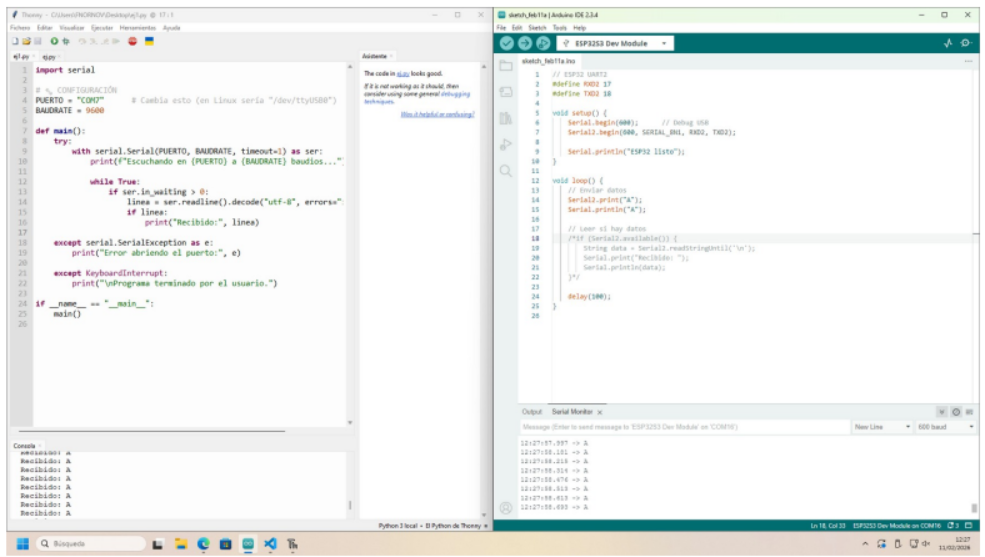
\includegraphics[width=0.8\textwidth]{assets/cap1/1.24.png}
\caption{Código de ejemplo para envío de datos por UART (PC o ESP32)}
\label{fig:codigo-envio}
\end{figure}

\subsubsection{Segunda parte: visualización con osciloscopio}

Se conectó la sonda del osciloscopio al pin TX (GPIO 18 o 17, según el caso) para observar la señal física. Enviando el carácter \texttt{'A'} (ASCII 0x41 = 01000001 en binario), se observó:

\begin{itemize}
    \item \textbf{Bit de inicio}: bajada de nivel (0 lógico).
    \item \textbf{Bits de datos}: \texttt{1} (LSB), \texttt{0}, \texttt{0}, \texttt{0}, \texttt{0}, \texttt{0}, \texttt{1}, \texttt{0} (MSB) — enviados en orden LSB primero, por lo que en la línea se lee \texttt{10000010} (bit0 a bit7).
    \item \textbf{Bit de parada}: retorno a nivel alto (1 lógico).
\end{itemize}

\begin{figure}[H]
\centering
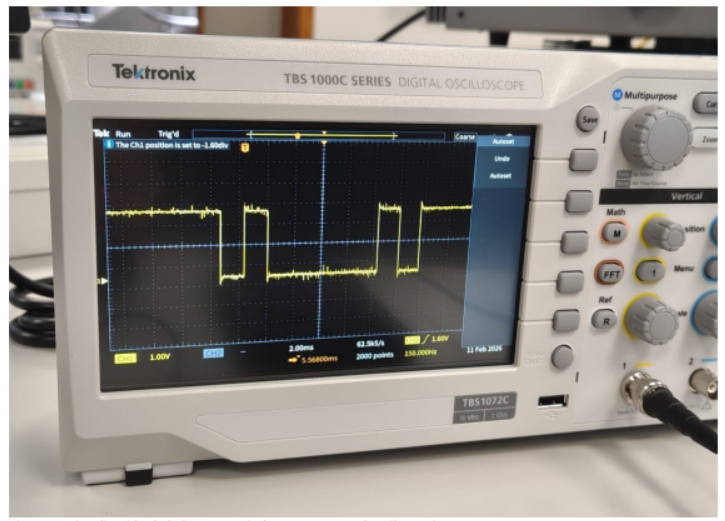
\includegraphics[width=0.8\textwidth]{assets/cap1/1.25.png}
\caption{Señal UART del carácter 'A' capturada en osciloscopio}
\label{fig:osciloscopio-a}
\end{figure}

\textbf{Decodificación manual}: la configuración utilizada fue 9600 8N1. Cada bit ocupa aproximadamente $1/9600 \approx 104\,\mu$s. En la pantalla del osciloscopio se puede medir la duración de cada pulso y confirmar que coincide con la velocidad configurada.

\subsubsection{Ampliación: comunicación bidireccional PC $\leftrightarrow$ ESP32}

Para la comunicación entre PC y ESP32 mediante el cable USB-TTL, se realizó el siguiente montaje:

\begin{itemize}
    \item Cable USB-TTL (verde = TX del cable) $\rightarrow$ GPIO 17 (RX de ESP32).
    \item GPIO 18 (TX de ESP32) $\rightarrow$ cable USB-TTL (blanco = RX del cable).
    \item GND común entre ambos dispositivos (esencial para la referencia de niveles).
\end{itemize}

\begin{figure}[H]
\centering
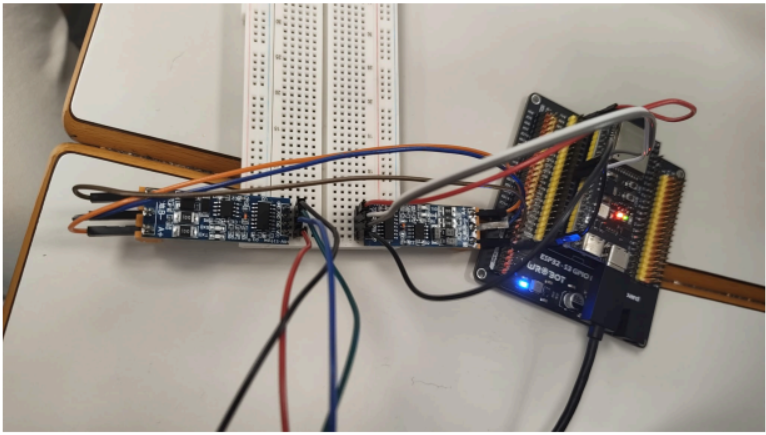
\includegraphics[width=0.8\textwidth]{assets/cap1/1.26.png}
\caption{Montaje físico para comunicación bidireccional PC $\leftrightarrow$ ESP32 por UART}
\label{fig:montaje-pc-esp32}
\end{figure}

\textbf{Problema detectado}: en una primera versión, se incluyó un carácter \texttt{\textbackslash n} (salto de línea) al final del mensaje. Esto generó una transición extra no deseada en la señal, visible en el osciloscopio. Al eliminarlo, la trama se ajustó exactamente al formato 8N1.

\textbf{Problema de buffer de recepción}: inicialmente, el código incluía una espera (delay) antes de leer. Esto causaba que varios bytes se acumularan en el buffer RX del ESP32 y se leyeran de golpe. Eliminando la espera, la lectura se hizo casi inmediata y se recibió correctamente un byte a la vez.

\subsection{Relación teoría-práctica}

\begin{table}[htbp]
\centering
\small
\caption{Conexión entre conceptos teóricos y elementos de la Práctica 1}
\begin{tabularx}{\textwidth}{@{}lX@{}}
\toprule
\textbf{Concepto teórico} & \textbf{Observación/aplicación en la práctica} \\
\midrule
Transmisión asíncrona & UART no usa reloj compartido; cada byte se sincroniza con su propio start bit \\
Formato de trama (start/stop) & Visualizado en osciloscopio: bajada (start), 8 bits, subida (stop) \\
Bit de paridad & Configuración 8N1: sin paridad; se podría cambiar a 8E1 o 8O1 \\
Velocidad (baudios) & 9600 baudios = $\sim$104\,$\mu$s por bit; medible en osciloscopio \\
Conexión P2P & Solo un PC y un ESP32; no es multidrop \\
Niveles TTL & ESP32 trabaja a 3.3V; el cable USB-TTL adapta a USB \\
Control de flujo (CTS/RTS) & GPIO 19 y 20 disponibles en ESP32, aunque no usados en esta práctica básica \\
Conexión cruzada TX$\leftrightarrow$RX & El TX del cable se conecta al RX del ESP32, y viceversa \\
\bottomrule
\end{tabularx}
\end{table}


\section{Práctica 2: Comunicación RS-232 entre ESP32-S3}
\label{sec:practica2}

\subsection{Objetivos}

La Práctica 2 amplía los conocimientos de la Práctica 1 introduciendo el estándar RS-232:
\begin{enumerate}
    \item Configurar la comunicación serie entre dos placas ESP32-S3 utilizando el protocolo RS-232.
    \item Observar las diferencias entre señales TTL (UART) y señales RS-232 (niveles de tensión e inversión).
    \item Verificar con osciloscopio la transmisión continua de un carácter y analizar su amplitud.
    \item Utilizar un cable \textbf{null-modem} para la comunicación directa entre dos DTE.
\end{enumerate}

\subsection{Material utilizado}

\begin{itemize}
    \item \textbf{Hardware}: 2 placas ESP32-S3-DevKitC-1, PC, 2 cables USB-TTL, 2 adaptadores TTL a RS-232, 2 adaptadores TTL a RS-485, cable null-modem, osciloscopio.
    \item \textbf{Software}: Arduino IDE.
\end{itemize}

\subsection{Desarrollo de la práctica}

\subsubsection{Primera parte: comunicación directa UART entre dos ESP32}

Se estableció una comunicación punto a punto entre dos placas ESP32-S3 mediante el puerto Serial2 (GPIO 16 y 17), conectando TX$\leftrightarrow$RX cruzado y GND común.

El código utilizado permite enviar o recibir simplemente comentando la parte no deseada:

\begin{lstlisting}[caption={Código ESP32 para transmisión/recepción por Serial2},label={lst:esp32-serial2}]
#define RXD2 17
#define TXD2 18

void setup() {
  Serial.begin(600);          // Debug USB
  Serial2.begin(600, SERIAL_8N1, RXD2, TXD2);
  Serial.println("ESP32 listo");
}

void loop() {
  // Enviar datos
  Serial2.print("S");
  Serial.println("S");
  
  // Leer si hay datos (comentar si solo se envia)
  /*if (Serial2.available()) {
    char data = Serial2.read('\n');
    Serial.print("Recibido: ");
    Serial.println(data);
  }*/
  
  delay(100);
}
\end{lstlisting}

\subsubsection{Segunda parte: verificación con osciloscopio}

Se conectó la sonda del osciloscopio al pin TX para verificar la transmisión continua del carácter \texttt{'S'} (ASCII 83 = 0x53 = \texttt{01010011} en binario).

\textbf{Análisis de la trama observada}:
\begin{itemize}
    \item El carácter \texttt{'S'} tiene valor binario: \texttt{01010011} (MSB $\rightarrow$ LSB).
    \item En UART, el \textbf{LSB se envía primero}, por lo que el orden de transmisión es: \texttt{11001010}.
    \item La trama completa es: \textbf{Start bit} (0) + \texttt{11001010} + \textbf{Stop bit} (1).
\end{itemize}

La señal observada en el osciloscopio coincidió exactamente con esta secuencia teórica.

\begin{figure}[H]
\centering
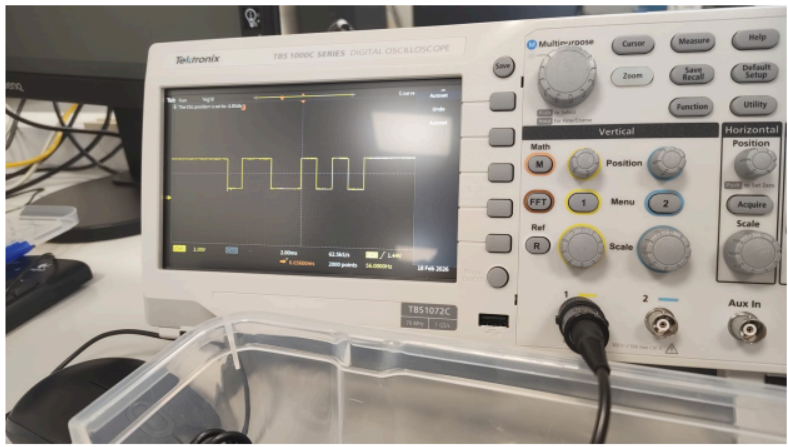
\includegraphics[width=0.8\textwidth]{assets/cap1/1.27.png}
\caption{Señal del carácter 'S' en osciloscopio (niveles TTL)}
\label{fig:osciloscopio-s}
\end{figure}

\subsubsection{Tercera parte: análisis de amplitud de la señal}

Se midieron los niveles de tensión de la señal TTL:

\begin{itemize}
    \item \textbf{Nivel alto}: aproximadamente $2.90\,\mathrm{V}$
    \item \textbf{Nivel bajo}: aproximadamente $0.70\,\mathrm{V}$
    \item \textbf{Amplitud pico a pico}: $\approx 2.20\,\mathrm{V}$
\end{itemize}

En condiciones ideales, una ESP32-S3 debería producir niveles de $0\,\mathrm{V}$ (bajo) y $3.3\,\mathrm{V}$ (alto). Las pequeñas desviaciones observadas se explican por:
\begin{itemize}
    \item Efecto de carga de la sonda del osciloscopio sobre el circuito.
    \item Caídas de tensión en el cableado.
    \item Referencia de masa no completamente estable.
    \item Ruido eléctrico ambiental, especialmente visible en los flancos.
\end{itemize}

\begin{figure}[H]
\centering
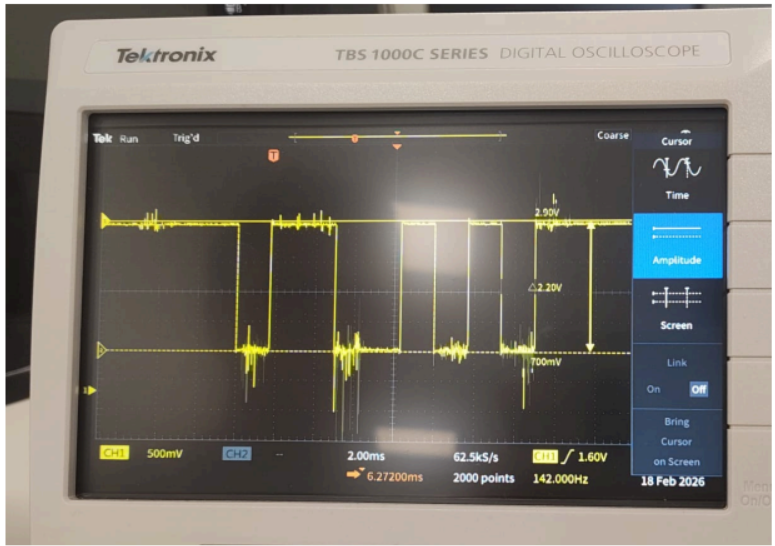
\includegraphics[width=0.8\textwidth]{assets/cap1/1.28.png}
\caption{Medida de amplitud de la señal TTL en osciloscopio}
\label{fig:amplitud-ttl}
\end{figure}

\subsubsection{Cuarta parte: uso del cable null-modem}

Un cable \textbf{null-modem} es un cable especial que cruza internamente las líneas TX y RX, permitiendo conectar dos equipos \textbf{DTE} (como dos ESP32) directamente sin necesidad de un DCE intermedio.

El montaje consiste en:
\begin{itemize}
    \item Conectar los adaptadores TTL$\rightarrow$RS-232 a cada ESP32.
    \item Unir ambos extremos mediante el cable null-modem.
    \item La conexión cruzada TX$\leftrightarrow$RX se realiza internamente en el cable.
\end{itemize}

Se comprobó que la comunicación funcionaba correctamente con el cable null-modem, y la señal observada en el osciloscopio coincidió con la obtenida anteriormente.

\begin{figure}[H]
\centering
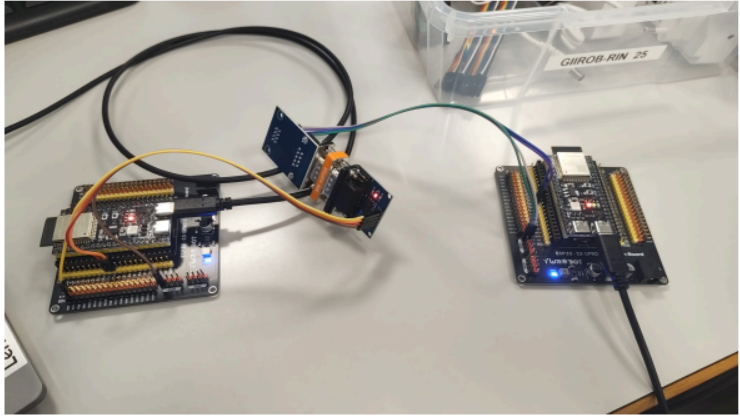
\includegraphics[width=0.8\textwidth]{assets/cap1/1.29.png}
\caption{Montaje con adaptadores TTL-RS-232 y cable null-modem}
\label{fig:null-modem}
\end{figure}

\subsection{Relación teoría-práctica: comparación UART vs. RS-232}

\begin{table}[htbp]
\centering
\small
\caption{Comparación entre Práctica 1 (UART/TTL) y Práctica 2 (RS-232)}
\begin{tabularx}{\textwidth}{@{}lXX@{}}
\toprule
\textbf{Aspecto} & \textbf{Práctica 1 (UART/TTL)} & \textbf{Práctica 2 (RS-232)} \\
\midrule
Nivel lógico 0 & 0V & $+$3V a $+$15V (típ. $+$12V) \\
Nivel lógico 1 & 3.3V & $-$3V a $-$15V (típ. $-$12V) \\
Inversión de señal & No & Sí \\
Distancia & $<$1 metro (USB-TTL) & Hasta 15 metros \\
Inmunidad al ruido & Baja & Alta \\
Hardware necesario & Cable USB-TTL & Adaptador TTL$\rightarrow$RS-232 \\
Conexión entre dos DTE & Cruzar TX-RX manualmente & Null-modem (cruce interno) \\
\bottomrule
\end{tabularx}
\end{table}


\section{Resumen de la Unidad 1}

\begin{itemize}
    \item Las \textbf{comunicaciones en serie} han sustituido a las paralelas en la mayoría de aplicaciones por su menor coste, mayor fiabilidad y capacidad para largas distancias.
    \item La \textbf{conexión diferencial} (balanceada) cancela el ruido común y es el estándar en entornos industriales.
    \item La \textbf{sincronización} puede ser asíncrona (UART), síncrona con reloj separado (SPI) o mediante recuperación desde los datos (CDR en USB/Ethernet).
    \item Los \textbf{protocolos} empaquetan los datos en tramas con delimitadores, direcciones y códigos de detección de errores.
    \item La \textbf{detección de errores} evoluciona desde el simple bit de paridad hasta el robusto CRC, pasando por el BCC.
    \item El \textbf{UART} es el protocolo asíncrono básico más usado en sistemas embebidos; su formato 8N1 es la configuración estándar.
    \item El estándar \textbf{RS-232} extiende el UART a niveles de tensión industriales ($\pm$12V), permitiendo distancias mayores y mayor inmunidad al ruido.
    \item La \textbf{Práctica 1} permite observar directamente la señal UART, confirmar el formato de trama, y establecer una comunicación real entre PC y microcontrolador.
    \item La \textbf{Práctica 2} demuestra la diferencia entre niveles TTL y RS-232, el uso de adaptadores, y la comunicación punto a punto entre dos microcontroladores.
\end{itemize}


% UNIDADES FUTURAS (placeholder)
%%%%%%%%%%%%%%%%%%%%%%%%%%%%%%%%%%%%%%%%%%%%%%%%%%%%%%%%%%%%%%%%%%%%%%%%%%%%%%%
%                         CAPÍTULO 2
%                  Redes Inalámbricas y Comunicaciones IoT
%%%%%%%%%%%%%%%%%%%%%%%%%%%%%%%%%%%%%%%%%%%%%%%%%%%%%%%%%%%%%%%%%%%%%%%%%%%%%%%

\chapter{Redes Inalámbricas y Comunicaciones IoT}

En los capítulos anteriores hemos estudiado cómo transmitir datos mediante cables:
señales eléctricas que viajan por hilos de cobre siguiendo reglas estrictas como
UART o RS-232. Sin embargo, en muchos entornos industriales y de automatización
resulta inviable o poco práctico tender cables entre cada dispositivo. Imagina un
almacén robotizado donde cientos de sensores de movimiento deben comunicarse con
una central, o una fábrica de alimentos donde los cables dificultan la higiene.

En este capítulo abordamos las \textbf{comunicaciones inalámbricas}, que utilizan
ondas de radio en lugar de conductores físicos para transmitir información. Nos
centraremos en las dos tecnologías más utilizadas en sistemas embebidos:
\textbf{Bluetooth Low Energy} (BLE) y \textbf{Wi-Fi}, y veremos cómo aplicarlas
en la práctica para construir una red de sensores IoT (Internet de las Cosas).


\section{Comunicaciones inalámbricas: ¿por qué eliminar los cables?}

La tendencia en la industria 4.0 es hacia la \textbf{desconexión física}: dispositivos
que se comunican sin cables, que se autoconfiguran y que pueden desplazarse.
Algunas ventajas de las comunicaciones inalámbricas son:

\begin{itemize}
    \item \textbf{Flexibilidad de instalación}: no es necesario diseñar canalizaciones
    ni prever la longitud exacta de los cables.
    \item \textbf{Movilidad}: robots, carretillas elevadoras o sensores portátiles pueden
    cambiar de ubicación sin restringirse por el cableado.
    \item \textbf{Reducción de costes de mantenimiento}: los cables físicos se degradan
    con el tiempo, especialmente en entornos con vibraciones, humedad o
    temperaturas extremas.
    \item \textbf{Escalabilidad}: es más sencillo añadir nuevos dispositivos a una red
    inalámbrica existente que tender nuevos cables.
\end{itemize}

Sin embargo, también existen inconvenientes:
\begin{itemize}
    \item \textbf{Interferencias}: otras redes, microondas o motores eléctricos pueden
    degradar la señal.
    \item \textbf{Seguridad}: las ondas de radio pueden ser interceptadas si no se
    cifran adecuadamente.
    \item \textbf{Consumo energético}: transmitir por radio consume más energía que
    enviar señales por un hilo.
    \item \textbf{Alcance limitado}: la potencia de transmisión está regulada y, en
    interiores, las paredes atenúan la señal.
\end{itemize}


\section{Bluetooth vs. Wi-Fi: dos filosofías, una misma banda}

Tanto Bluetooth como Wi-Fi operan en la banda de radio de \textbf{2.4 GHz} (aunque
Wi-Fi también puede usar 5 GHz y 6 GHz en versiones modernas). A pesar de
compartir el mismo espectro, están diseñados para propósitos muy diferentes.

\begin{definicion}{Bluetooth y Wi-Fi}
\textbf{Bluetooth} es un estándar de comunicación inalámbrica de corto alcance y
bajo consumo, pensado para crear redes de área personal (PAN) entre dispositivos
próximos.

\textbf{Wi-Fi} es un estándar de comunicación inalámbrica de mayor alcance y
velocidad, diseñado para crear redes de área local (LAN) que permiten a
múltiples dispositivos acceder a internet o compartir recursos de forma simultánea.
\end{definicion}

\begin{table}[htbp]
\centering
\small
\caption{Comparación entre Bluetooth y Wi-Fi}
\begin{tabularx}{\textwidth}{@{}lXX@{}}
\toprule
\textbf{Característica} & \textbf{Bluetooth (BLE)} & \textbf{Wi-Fi} \\
\midrule
Alcance típico & 10--100 m (según clase) & 30--100 m (interior) \\
Velocidad de datos & Hasta 2 Mb/s (BLE 5.0) & Hasta varios Gb/s (Wi-Fi 6) \\
Consumo de energía & Muy bajo (meses con pila) & Alto (necesita alimentación) \\
Topología típica & Punto a punto (1 maestro, 7 esclavos) & Estrella (AP + múltiples clientes) \\
Uso principal & Periféricos, sensores, wearables & Acceso a internet, streaming, redes corporativas \\
Complejidad de protocolo & Simple (GATT) & Compleja (TCP/IP, HTTP, etc.) \\
Interferencias en 2.4 GHz & Alta (comparte banda con Wi-Fi) & Alta (comparte banda con Bluetooth) \\
\bottomrule
\end{tabularx}
\end{table}

\textbf{¿Cuándo usar cada uno?}
\begin{itemize}
    \item Usa \textbf{Bluetooth} cuando necesites conectar un sensor o un periférico
    a un dispositivo central, con bajo consumo y sin necesidad de acceso a internet.
    Ejemplos: auriculares inalámbricos, pulsómetros, sensores de temperatura portátiles.
    \item Usa \textbf{Wi-Fi} cuando el dispositivo necesite enviar datos a un servidor
    en la nube, recibir comandos remotos o formar parte de una red corporativa.
    Ejemplos: cámaras de videovigilancia, termostatos inteligentes, paneles de control.
\end{itemize}


\section{Bluetooth Low Energy (BLE)}

\subsection{¿Qué es BLE?}

Bluetooth Low Energy (BLE), también conocido como Bluetooth Smart, es una versión
del estándar Bluetooth optimizada para un consumo de energía mínimo. No es
compatible a nivel de protocolo con el Bluetooth clásico (el de los auriculares), pero
comparte la misma banda de radio.

\begin{definicion}{Bluetooth Low Energy (BLE)}
BLE es un protocolo de comunicación inalámbrica de corto alcance que permite la
transmisión de pequeños paquetes de datos con un consumo de energía extremadamente
bajo. Es ideal para dispositivos alimentados por baterías que deben operar durante
meses o años sin recargarse.
\end{definicion}

En BLE, los dispositivos desempeñan dos roles principales:
\begin{itemize}
    \item \textbf{Periférico (Peripheral)}: dispositivo que ofrece datos. Suele ser el sensor
    o el actuador.
    \item \textbf{Central (Central)}: dispositivo que solicita y recibe datos. Suele ser un
    teléfono, un PC o un gateway IoT.
\end{itemize}

\subsection{Arquitectura GATT: servicios y características}

BLE organiza la información mediante una estructura jerárquica conocida como
\textbf{GATT} (Generic Attribute Profile):

\begin{enumerate}
    \item \textbf{Perfil (Profile)}: conjunto de servicios predefinidos para un uso específico
    (por ejemplo, un perfil de pulsómetro).
    \item \textbf{Servicio (Service)}: agrupación lógica de características. Por ejemplo, un
    ``servicio de temperatura''.
    \item \textbf{Característica (Characteristic)}: el dato concreto. Puede ser una
    temperatura, una cadena de texto o un valor de configuración.
    \item \textbf{Descriptor (Descriptor)}: metadatos adicionales sobre una característica,
    como su formato o unidades.
\end{enumerate}

Cada servicio y característica se identifica mediante un \textbf{UUID} (Universally Unique
Identifier), un código de 128 bits que garantiza que no haya colisiones entre
aplicaciones diferentes.

\begin{definicion}{UUID en BLE}
Un \textbf{UUID} (Universally Unique Identifier) es un identificador numérico de 128 bits
que se utiliza para distinguir de forma única servicios, características y descriptores
dentro de una aplicación BLE. Los UUIDs pueden ser estandarizados (16 o 32 bits) o
customizados por el desarrollador (128 bits).
\end{definicion}

\subsection{Advertising y escaneo}

Un periférico BLE no puede ser conectado directamente. Primero debe anunciar su
presencia mediante un proceso llamado \textbf{advertising} (difusión): envía paquetes
periódicos de anuncio que contienen su nombre, el UUID de sus servicios y otros
datos.

Una central que desea conectarse realiza un \textbf{escaneo} (scanning): escucha los
paquetes de anuncio hasta encontrar un dispositivo con el UUID que busca. Una vez
encontrado, se establece la conexión.

\subsection{Notificaciones y lecturas}

Las características BLE pueden tener diferentes propiedades:
\begin{itemize}
    \item \textbf{READ}: la central puede leer el valor explícitamente.
    \item \textbf{WRITE}: la central puede escribir un valor.
    \item \textbf{NOTIFY}: el periférico envía el valor automáticamente cada vez que cambia,
    sin que la central tenga que pedirlo.
\end{itemize}

Las notificaciones son especialmente útiles en IoT: el sensor envía una nueva lectura
de temperatura cada vez que está disponible, sin que el receptor tenga que estar
constantemente preguntando.


\section{Wi-Fi en sistemas embebidos}

\subsection{Modos de operación}

Un dispositivo Wi-Fi puede funcionar en dos modos principales:

\begin{itemize}
    \item \textbf{STA (Station)}: el dispositivo se conecta a un punto de acceso (AP)
    existente, como un router. Es el modo más común para sensores IoT.
    \item \textbf{AP (Access Point)}: el dispositivo crea su propia red Wi-Fi a la que
    otros dispositivos pueden conectarse. Útil para configuración inicial.
\end{itemize}

\subsection{Protocolo HTTP para IoT}

En la práctica, cuando un dispositivo embebido con Wi-Fi necesita comunicarse, lo
hace a través del protocolo \textbf{HTTP} (HyperText Transfer Protocol), el mismo que
utiliza un navegador web para cargar páginas.

\begin{definicion}{HTTP en IoT}
HTTP es el protocolo de comunicación que permite a un cliente (por ejemplo, una
ESP32 o un navegador) solicitar recursos a un servidor. En el contexto IoT, un sensor
puede actuar como \textbf{servidor HTTP}, respondiendo a peticiones con datos en formato
texto, JSON o XML.
\end{definicion}

El flujo típico es:
\begin{enumerate}
    \item El dispositivo sensor se conecta a la red Wi-Fi (modo STA).
    \item Se le asigna una dirección IP por DHCP.
    \item Inicia un servidor HTTP en un puerto (normalmente el 80).
    \item Define rutas, como \texttt{/temperatura}, que devuelven el valor del sensor.
    \item Un cliente (otra ESP32, un PC o un smartphone) realiza una petición
    \texttt{GET} a esa IP y ruta, y recibe el dato.
\end{enumerate}

\subsection{Redes corporativas y seguridad}

En entornos universitarios o industriales, las redes Wi-Fi suelen estar protegidas
mediante autenticación (WPA2-PSK, WPA2-Enterprise) o listas de control de acceso
(MAC filtering). Esto puede complicar la conexión de dispositivos IoT, ya que no todos
los sistemas embebidos soportan los métodos de autenticación más avanzados.

En la práctica, una solución común cuando la red corporativa es problemática es
utilizar un \textbf{hotspot móvil} (punto de acceso creado por un teléfono), que permite
controlar directamente qué dispositivos se conectan.


\section{Sensor de temperatura y humedad DHT11}

El \textbf{DHT11} es un sensor digital de bajo coste que mide temperatura y humedad
relativa del aire. Es muy popular en proyectos educativos y de prototipado porque
su conexión es simple (solo necesita un pin de datos y alimentación) y proporciona
valores directamente en formato digital, sin necesidad de conversión analógica.

\begin{definicion}{DHT11}
El DHT11 es un sensor digital compuesto que incluye un elemento resistivo para medir
humedad y un termistor para medir temperatura. Su resolución es de 1 grado Celsius y
1 \% de humedad relativa, con un rango de 0 a 50 grados Celsius. El tiempo mínimo
entre lecturas es de aproximadamente 1 segundo.
\end{definicion}

Aunque el DHT11 no es el sensor más preciso del mercado (el DHT22 o el SHT30 son
más exactos), su simplicidad y precio lo hacen ideal para aprender los fundamentos
de la adquisición de datos y la transmisión de sensores.


\section{Práctica 3: Comunicaciones Inalámbricas}
\label{sec:practica3}

\subsection{Objetivos}

El objetivo de esta práctica es diseñar e implementar dos aplicaciones que transmitan
la temperatura ambiente del laboratorio a una red:

\begin{enumerate}
    \item Una aplicación basada en \textbf{Bluetooth BLE} que permita la comunicación
    directa entre dos placas ESP32-S3 sin cables.
    \item Una aplicación basada en \textbf{Wi-Fi} que permita acceder a la temperatura
    mediante una petición HTTP desde cualquier dispositivo conectado a la misma red.
\end{enumerate}

\subsection{Material utilizado}

\begin{itemize}
    \item \textbf{Hardware}: Ordenador, dos placas ESP32-S3-DevKitC-1 N16R8, un sensor
    de temperatura DHT11.
    \item \textbf{Software}: Arduino IDE con las librerías \texttt{DHT}, \texttt{BLEDevice}
    y \texttt{WebServer}.
    \item \textbf{Red}: Conexión a la red inalámbrica \texttt{UPV-PSK} (o un hotspot móvil
    como alternativa).
\end{itemize}

\subsection{Desarrollo de la práctica}

\subsubsection{Primera parte: lectura del sensor DHT11}

Antes de enviar datos por el aire, es necesario obtenerlos de forma fiable. El primer
programa tiene como objetivo leer la temperatura del sensor DHT11 conectado al
pin 2 de la ESP32 y mostrarla por el puerto serie.

El código es sencillo: se inicializa el sensor, se realiza una lectura cada 2 segundos
y se comprueba que el valor sea válido (el DHT11 puede devolver errores ocasionales
si no se respeta el tiempo de muestreo).

\begin{lstlisting}[caption={Lectura del sensor DHT11},label={lst:dht11-lectura}]
#include <DHT.h>

#define DHTPIN 2
#define DHTTYPE DHT11

DHT dht(DHTPIN, DHTTYPE);

void setup() {
  Serial.begin(115200);
  dht.begin();
  Serial.println("Sensor DHT11 inicializado.");
}

void loop() {
  float temperatura = dht.readTemperature();

  if (isnan(temperatura)) {
    Serial.println("Error leyendo el DHT11");
  } else {
    Serial.print("Temperatura: ");
    Serial.print(temperatura);
    Serial.println(" C");
  }
  delay(2000);
}
\end{lstlisting}

\begin{figure}[H]
\centering
\fbox{\parbox{0.8\textwidth}{\centering\vspace{1.5cm}\textit{TODO: Anadir fotografia del montaje fisico con la ESP32-S3 y el sensor DHT11 conectado.}\vspace{1.5cm}}}
\caption{Montaje fisico del sensor DHT11 con la ESP32-S3}
\label{fig:montaje-dht11}
\end{figure}

\subsubsection{Segunda parte: servidor BLE}

Una vez confirmado que el sensor funciona, se implementa un \textbf{servidor BLE}
sobre una de las ESP32-S3. Este servidor crea un servicio de temperatura con dos
características:

\begin{itemize}
    \item \textbf{Caracteristica 1}: envia la temperatura como valor numerico (float).
    \item \textbf{Caracteristica 2}: envia la temperatura como cadena de texto descriptiva.
\end{itemize}

Ambas caracteristicas tienen notificaciones activadas, lo que significa que cualquier
cliente conectado recibira los datos automaticamente sin tener que solicitarlos.

El servidor tambien gestiona la reconexion: si el cliente se desconecta, la ESP32
vuelve a anunciarse (advertising) para aceptar nuevas conexiones.

\begin{lstlisting}[caption={Servidor BLE de temperatura (extracto)},label={lst:ble-server}]
// UUIDs del servicio y caracteristicas
#define SERVICE_UUID        "8628b276-4bba-420a-ab99-dd69945408bf"
#define CHARACTERISTIC_UUID_1 "6cb1114c-4410-4757-85af-b064b3cc689a"
#define CHARACTERISTIC_UUID_2 "a1642e22-4f4e-41de-b173-b5bdb099f12c"

// Inicializar BLE
BLEDevice::init("ESP32_Temperatura");
pServer = BLEDevice::createServer();
pServer->setCallbacks(new MyServerCallbacks());

BLEService *pService = pServer->createService(SERVICE_UUID);

// Caracteristica numerica con notificaciones
pCharacteristic_1 = pService->createCharacteristic(
  CHARACTERISTIC_UUID_1,
  BLECharacteristic::PROPERTY_NOTIFY
);
pBLE2902_1 = new BLE2902();
pBLE2902_1->setNotifications(true);
pCharacteristic_1->addDescriptor(pBLE2902_1);

pService->start();
BLEDevice::startAdvertising();
\end{lstlisting}

En el bucle principal, si hay un cliente conectado, el servidor lee el DHT11 y
envia el valor por ambas caracteristicas:

\begin{lstlisting}[caption={Envio de temperatura por BLE},label={lst:ble-envio}]
if (deviceConnected) {
  float temperatura = dht.readTemperature();
  if (isnan(temperatura)) {
    Serial.println("Error leyendo el DHT11");
    delay(2000);
    return;
  }

  // Enviar como valor numerico
  pCharacteristic_1->setValue(temperatura);
  pCharacteristic_1->notify();

  // Enviar como texto descriptivo
  String mensaje = "Temperatura actual: " + String(temperatura) + " C";
  pCharacteristic_2->setValue(mensaje.c_str());
  pCharacteristic_2->notify();

  delay(2000);
}
\end{lstlisting}

\subsubsection{Tercera parte: cliente BLE}

La segunda ESP32-S3 actua como \textbf{cliente BLE}. Su mision es escanear el entorno
buscando un dispositivo que anuncie el \texttt{SERVICE\_UUID} del servidor, conectarse
a el, suscribirse a las notificaciones de una de las caracteristicas y mostrar el
dato recibido por el puerto serie.

\begin{lstlisting}[caption={Cliente BLE de temperatura (extracto)},label={lst:ble-client}]
// UUIDs (iguales que en el servidor)
#define SERVICE_UUID        "8628b276-4bba-420a-ab99-dd69945408bf"
#define CHARACTERISTIC_UUID "a1642e22-4f4e-41de-b173-b5bdb099f12c"

// Callback cuando se detecta el servidor
class MyAdvertisedDeviceCallbacks: public BLEAdvertisedDeviceCallbacks {
  void onResult(BLEAdvertisedDevice advertisedDevice) {
    if (advertisedDevice.haveServiceUUID() &&
        advertisedDevice.isAdvertisingService(BLEUUID(SERVICE_UUID))) {
      Serial.println("Servidor encontrado");
      pServerAddress = new BLEAddress(advertisedDevice.getAddress());
      doConnect = true;
      advertisedDevice.getScan()->stop();
    }
  }
};

// Callback cuando llegan notificaciones
static void notifyCallback(
  BLERemoteCharacteristic* pBLERemoteCharacteristic,
  uint8_t* pData, size_t length, bool isNotify) {
  String mensaje = "";
  for (int i = 0; i < length; i++) {
    mensaje += (char)pData[i];
  }
  Serial.print("Mensaje recibido: ");
  Serial.println(mensaje);
}
\end{lstlisting}

\begin{figure}[H]
\centering
\fbox{\parbox{0.8\textwidth}{\centering\vspace{1.5cm}\textit{TODO: Anadir captura de pantalla del monitor serie del cliente BLE mostrando la temperatura recibida.}\vspace{1.5cm}}}
\caption{Monitor serie del cliente BLE recibiendo temperatura}
\label{fig:ble-cliente-serie}
\end{figure}

\subsubsection{Cuarta parte: servidor y cliente Wi-Fi}

La alternativa a BLE es utilizar \textbf{Wi-Fi} para crear una red de sensores mas
abierta. En este caso, la ESP32-S3 que lleva el DHT11 se conecta a la red
\texttt{UPV-PSK} y actua como \textbf{servidor web HTTP} en el puerto 80.

Cada vez que un cliente visita la URL \texttt{http://IP\_DEL\_ESP32/temperatura},
el servidor lee el sensor y responde con el valor de temperatura como texto plano.

\begin{lstlisting}[caption={Servidor Wi-Fi de temperatura},label={lst:wifi-server}]
#include <WiFi.h>
#include <WebServer.h>
#include <DHT.h>

#define DHTPIN 2
#define DHTTYPE DHT11
DHT dht(DHTPIN, DHTTYPE);

const char* ssid = "UPV-PSK";
const char* password = "C0n3ct4nd0s3_m0l4!";
WebServer server(80);

void handleTemperatura() {
  float temperatura = dht.readTemperature();
  if (isnan(temperatura)) {
    server.send(500, "text/plain", "Error leyendo sensor");
    return;
  }
  server.send(200, "text/plain", String(temperatura));
}

void setup() {
  Serial.begin(115200);
  dht.begin();
  WiFi.begin(ssid, password);
  while (WiFi.status() != WL_CONNECTED) {
    delay(500);
    Serial.print(".");
  }
  Serial.println("\nConectado!");
  Serial.print("IP del servidor: ");
  Serial.println(WiFi.localIP());

  server.on("/temperatura", handleTemperatura);
  server.begin();
}

void loop() {
  server.handleClient();
}
\end{lstlisting}

Por otro lado, la segunda ESP32 (o cualquier ordenador) actua como \textbf{cliente
HTTP}. Se conecta a la misma red Wi-Fi, construye la URL a partir de la IP del
servidor, realiza una peticion \texttt{GET} cada 2 segundos y muestra la respuesta.

\begin{lstlisting}[caption={Cliente Wi-Fi de temperatura},label={lst:wifi-client}]
#include <WiFi.h>
#include <HTTPClient.h>

const char* ssid = "UPV-PSK";
const char* password = "C0n3ct4nd0s3_m0l4!";
const char* serverIP = "192.168.1.42";

void setup() {
  Serial.begin(115200);
  WiFi.begin(ssid, password);
  while (WiFi.status() != WL_CONNECTED) {
    delay(500);
    Serial.print(".");
  }
  Serial.println("\nConectado a la red WiFi");
}

void loop() {
  if (WiFi.status() == WL_CONNECTED) {
    HTTPClient http;
    String url = String("http://") + serverIP + "/temperatura";
    http.begin(url);
    int httpResponseCode = http.GET();

    if (httpResponseCode > 0) {
      String temperatura = http.getString();
      Serial.print("Temperatura recibida: ");
      Serial.println(temperatura + " C");
    } else {
      Serial.print("Error en la conexion: ");
      Serial.println(httpResponseCode);
    }
    http.end();
  }
  delay(2000);
}
\end{lstlisting}

\begin{figure}[H]
\centering
\fbox{\parbox{0.8\textwidth}{\centering\vspace{1.5cm}\textit{TODO: Anadir captura de pantalla del monitor serie del cliente Wi-Fi mostrando la temperatura recibida.}\vspace{1.5cm}}}
\caption{Monitor serie del cliente Wi-Fi recibiendo temperatura via HTTP}
\label{fig:wifi-cliente-serie}
\end{figure}

\subsection{Problemas encontrados}

Durante la practica, la conexion a la red \texttt{UPV-PSK} resulto en ocasiones
bastante complicada. Frecuentemente aparecian \textbf{timeouts} que obligaban a
reiniciar el proceso de conexion. Tras analizar la situacion, se concluyo que la red
tiene un sistema de \textbf{control de acceso} que mantiene una lista de dispositivos
admitidos. Algunos equipos quedaban en espera dentro de esta lista, lo que impedia
que se conectaran correctamente.

Como \textbf{alternativa}, se opto por utilizar el \textbf{hotspot de un telefono movil}.
Esto permitio controlar directamente que dispositivos podian conectarse, agilizando
el proceso y asegurando que la practica pudiera realizarse sin depender de las
limitaciones de la red de la universidad. Esta solucion demostro ser mas fiable y
rapida para el desarrollo de los experimentos.

\subsection{Relacion teoria-practica: BLE vs. Wi-Fi en la practica}

\begin{table}[htbp]
\centering
\small
\caption{Conexion entre conceptos teoricos y elementos de la Practica 3}
\begin{tabularx}{\textwidth}{@{}lX@{}}
\toprule
\textbf{Concepto teorico} & \textbf{Observacion/aplicacion en la practica} \\
\midrule
Bluetooth BLE & Se implemento un servidor/periférico BLE con servicio de temperatura y un cliente/central que recibe notificaciones \\
UUID (GATT) & Cada servicio y caracteristica tiene un UUID unico de 128 bits para identificarlos sin ambiguedad \\
Advertising & El servidor BLE envia paquetes de anuncio para que el cliente pueda descubrirlo \\
Notificaciones BLE & La temperatura se envia automaticamente al cliente sin que este tenga que solicitarla explicitamente \\
Wi-Fi (modo STA) & La ESP32 se conecta a la red UPV-PSK como estacion, obteniendo una IP por DHCP \\
Servidor HTTP & La ESP32 actua como servidor web en el puerto 80, respondiendo peticiones GET en la ruta /temperatura \\
Cliente HTTP & La segunda ESP32 realiza peticiones GET periodicas para obtener la temperatura del servidor \\
Red corporativa IoT & Se evidencio el problema del control de acceso en redes universitarias, resuelto con un hotspot alternativo \\
Sensor DHT11 & Proporciona el dato de temperatura real que alimenta tanto al servidor BLE como al servidor Wi-Fi \\
Consumo energetico & BLE consume menos que Wi-Fi, aunque en esta practica ambas placas estaban alimentadas por USB \\
\bottomrule
\end{tabularx}
\end{table}


\section{Resumen de la Unidad 2}

\begin{itemize}
    \item Las \textbf{comunicaciones inalambricas} eliminan la necesidad de cableado
    fisico, ofreciendo flexibilidad y movilidad, aunque introducen desafios como
    interferencias, seguridad y consumo energetico.
    \item \textbf{Bluetooth} y \textbf{Wi-Fi} comparten la banda de 2.4 GHz pero estan
    disenados para propositos distintos: BLE es ideal para sensores de bajo consumo
    a corta distancia, mientras que Wi-Fi proporciona mayor alcance y velocidad para
    acceso a redes y a internet.
    \item \textbf{BLE} organiza los datos mediante el perfil GATT, utilizando servicios
    y caracteristicas identificados por UUIDs. Las notificaciones permiten enviar
    datos de forma automatica sin polling.
    \item \textbf{Wi-Fi} en sistemas embebidos permite crear servidores HTTP que
    exponen datos de sensores a traves de peticiones web estandar, facilitando la
    integracion con aplicaciones y plataformas en la nube.
    \item La \textbf{Practica 3} demuestra la viabilidad de ambas tecnologias para
    transmitir datos de temperatura en tiempo real, comparando el enfoque punto a
    punto de BLE con el enfoque cliente-servidor web de Wi-Fi.
    \item Las \textbf{redes corporativas IoT} pueden presentar barreras de acceso
    (control de dispositivos, timeouts) que requieren soluciones alternativas como
    hotspots moviles para el desarrollo de prototipos.
\end{itemize}

%%%%%%%%%%%%%%%%%%%%%%%%%%%%%%%%%%%%%%%%%%%%%%%%%%%%%%%%%%%%%%%%%%%%%%%%%%%%%%%
%                         CAPITULO 3
%                  Redes de Area Local y Encaminamiento
%%%%%%%%%%%%%%%%%%%%%%%%%%%%%%%%%%%%%%%%%%%%%%%%%%%%%%%%%%%%%%%%%%%%%%%%%%%%%%%

\chapter{Redes de Area Local y Encaminamiento}

Hasta ahora hemos estudiado como comunicar dos dispositivos mediante cables
(UART, RS-232) y mediante ondas de radio (Bluetooth, Wi-Fi). Sin embargo, en
un entorno industrial real no hay solo dos dispositivos: hay cientos de
ordenadores, PLCs, sensores, servidores y camaras, todos conectados entre si
y con la necesidad de compartir informacion.

En este capitulo abordamos las \textbf{redes de computadores} desde una
perspectiva arquitectonica: como se organizan fisicamente, como se identifican
los dispositivos, como se toman las decisiones de donde enviar los paquetes de
datos y que dispositivos permiten que una red se conecte con otra.


\section{TCP/IP}

El modelo \textbf{TCP/IP} es la arquitectura de comunicaciones de Internet. En su version simplificada, consta de cuatro capas:

\begin{definicion}
\textbf{IP (Internet Protocol)} es el protocolo que obtiene y define la direccion IP del destino. Actua como un numero de telefono asignado a cada dispositivo en la red.

\textbf{TCP (Transmission Control Protocol)} transporta y enruta los datos a traves de la red, garantizando la entrega al destino que IP ha definido. Es la tecnologia que permite establecer la comunicacion entre dos puntos.
\end{definicion}

\subsection{Capas del modelo TCP/IP}

\begin{itemize}
    \item \textbf{Capa de aplicacion}: protocolos para aplicaciones de red (HTTP, FTP, DNS, SMTP, etc.).
    \item \textbf{Capa de transporte}: transmision de datos entre procesos. Protocolos: TCP (fiable) y UDP (rapido).
    \item \textbf{Capa de Internet (Red)}: direccionamiento y encaminamiento de paquetes. Protocolo: IP.
    \item \textbf{Capa de enlace de datos}: transmision fisica por el medio (cable, fibra, radio).
\end{itemize}

\begin{figure}[H]
\centering
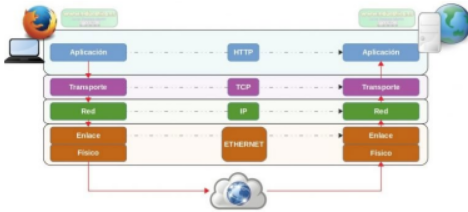
\includegraphics[width=0.8\textwidth]{assets/cap3/3.1.png}
\caption{Pila de protocolos TCP/IP}
\label{fig:pila-tcpip}
\end{figure}


\section{TCP}

\begin{definicion}
\textbf{TCP} (Transmission Control Protocol) es un protocolo de la capa de transporte \textbf{orientado a conexion}. Hace fiable la comunicacion: si falta un paquete o hay error, solicita el reenvio. Solo entrega los datos al nivel superior si estan completos.
\end{definicion}

\begin{figure}[H]
\centering
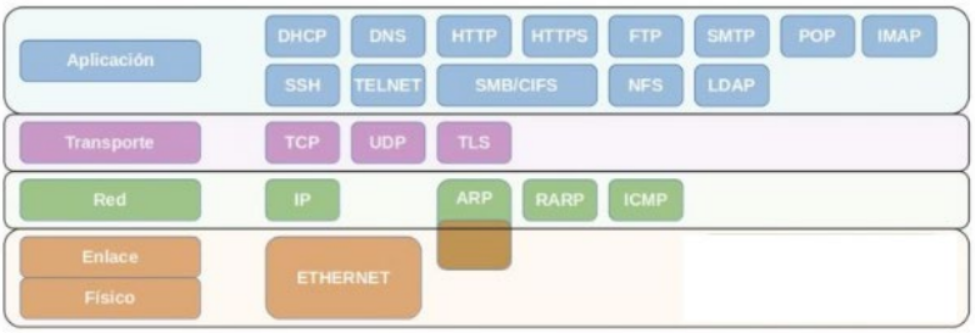
\includegraphics[width=0.8\textwidth]{assets/cap3/3.2.png}
\caption{Funcionamiento de TCP orientado a conexion}
\label{fig:funcionamiento-tcp}
\end{figure}


\section{UDP}

\begin{definicion}
\textbf{UDP} (User Datagram Protocol) es un protocolo de la capa de transporte \textbf{sin conexion}, mas rapido que TCP. No garantiza recepcion ni orden de los datos. Es adecuado cuando la velocidad importa mas que la fiabilidad: juegos en linea, streaming, DNS.
\end{definicion}

\begin{table}[htbp]
\centering
\small
\caption{Comparativa TCP vs UDP}
\begin{tabularx}{\textwidth}{@{}lXX@{}}
\toprule
\textbf{Caracteristica} & \textbf{TCP} & \textbf{UDP} \\
\midrule
Conexion & Orientado a conexion & Sin conexion \\
Fiabilidad & Fiable (reenvia paquetes perdidos) & No fiable \\
Orden de entrega & Entrega ordenada & Sin orden garantizado \\
Latencia & Mayor latencia & Baja latencia \\
\bottomrule
\end{tabularx}
\end{table}

\begin{figure}[H]
\centering
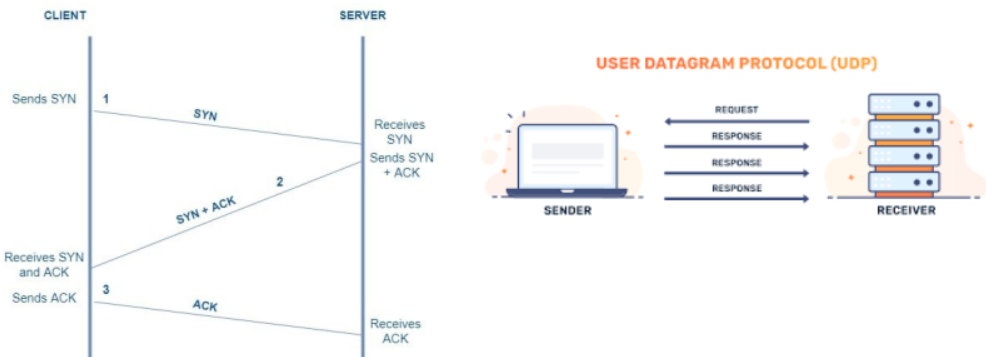
\includegraphics[width=0.8\textwidth]{assets/cap3/3.3.png}
\caption{Comparativa TCP vs UDP}
\label{fig:comparativa-tcp-udp}
\end{figure}


\section{Direccionamiento IP}

Cada dispositivo en una red tiene un \textbf{identificador unico}: la direccion IP. Ademas, cada tarjeta de red dispone de una \textbf{direccion MAC} (Media Access Control), una direccion fisica unica de 48 bits asignada por el fabricante.

\begin{definicion}
Una \textbf{direccion IP} es un identificador numerico que permite localizar un dispositivo dentro de la red y enrutar los paquetes hacia el.
\end{definicion}

\subsection{Representacion IP}

\begin{itemize}
    \item Secuencia de \textbf{32 bits} (4 octetos).
    \item Notacion decimal punteada: \texttt{192.168.1.2}.
    \item Cada octeto: 8 bits, valores de 0 a 255.
\end{itemize}

\begin{figure}[H]
\centering
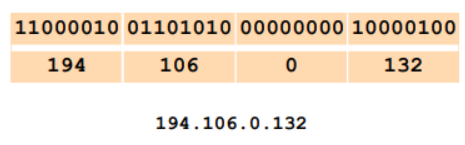
\includegraphics[width=0.8\textwidth]{assets/cap3/3.4.png}
\caption{Formato de una direccion IP de 32 bits}
\label{fig:formato-ip}
\end{figure}

\subsection{IP Dinamica}

Asignada por un servidor \textbf{DHCP} al conectarse. Cambia cada vez que el dispositivo se reconecta. Tipica en hogares.

\subsection{IP Fija}

No cambia. Usada en empresas para identificar servidores, administradores, etc.


\section{Direccionamiento IP con Clase}

Historicamente, las direcciones IP se dividieron en clases. Cada IP tiene dos partes: \textbf{red} y \textbf{host}. Los octetos dedicados a cada una definen la clase.

\begin{figure}[H]
\centering
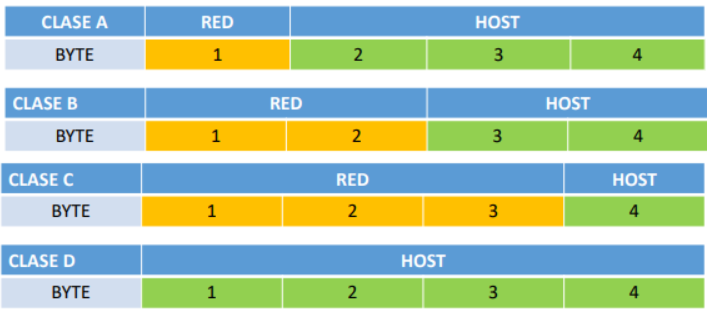
\includegraphics[width=0.8\textwidth]{assets/cap3/3.5.png}
\caption{Estructura de direcciones IP con clase}
\label{fig:ip-con-clase}
\end{figure}

\subsection{Clase A}

\begin{itemize}
    \item Red: 1.\textsuperscript{er} octeto. Host: 3 octetos restantes.
    \item 1.\textsuperscript{er} bit siempre \texttt{0}.
    \item Rango: 1 -- 126.
    \item Hasta ~16 millones de hosts por red.
\end{itemize}

\subsection{Clase B}

\begin{itemize}
    \item Red: 1.\textsuperscript{er} y 2.\textsuperscript{o} octeto. Host: 3.\textsuperscript{er} y 4.\textsuperscript{o} octeto.
    \item 1.\textsuperscript{er} bits siempre \texttt{10}.
    \item Rango: 128 -- 191.
    \item Redes de tamano moderado a grande.
\end{itemize}

\subsection{Clase C}

\begin{itemize}
    \item Red: 1.\textsuperscript{er}, 2.\textsuperscript{o} y 3.\textsuperscript{er} octeto. Host: 4.\textsuperscript{o} octeto.
    \item 1.\textsuperscript{er} bits siempre \texttt{110}.
    \item Rango: 192 -- 223.
    \item Maximo 254 hosts por red. Uso mas frecuente.
\end{itemize}

\subsection{Clase D}

\begin{itemize}
    \item Para \textbf{multicast}: un paquete se envia a un grupo predefinido de IPs.
    \item 1.\textsuperscript{er} bits siempre \texttt{1110}.
    \item Rango: 224 -- 239.
\end{itemize}

\subsection{Clase E}

\begin{itemize}
    \item Reservada para investigacion (IETF).
    \item Rango: 240 -- 255.
\end{itemize}

\subsection{Resumen de clases}

\begin{table}[htbp]
\centering
\small
\caption{Resumen de clases de direcciones IP}
\begin{tabularx}{\textwidth}{@{}lXX@{}}
\toprule
\textbf{Clase} & \textbf{Rango (1.\textsuperscript{er} octeto)} & \textbf{Uso} \\
\midrule
A & 1 -- 126 & Redes muy grandes (~16M hosts) \\
B & 128 -- 191 & Redes medianas (65.534 hosts) \\
C & 192 -- 223 & Redes pequenas (254 hosts) \\
D & 224 -- 239 & Multicast \\
E & 240 -- 255 & Investigacion \\
\bottomrule
\end{tabularx}
\end{table}

\subsection{Direcciones de redes privadas}

\begin{table}[htbp]
\centering
\small
\caption{Direcciones de redes privadas}
\begin{tabularx}{\textwidth}{@{}lX@{}}
\toprule
\textbf{Clase} & \textbf{Rango} \\
\midrule
A & 10.0.0.0 -- 10.255.255.255 \\
B & 172.16.0.0 -- 172.31.255.255 \\
C & 192.168.0.0 -- 192.168.255.255 \\
\bottomrule
\end{tabularx}
\end{table}

\subsection{Direcciones de red y especiales}

\begin{itemize}
    \item \textbf{Direccion de red}: todos los bits de host a 0 (ej. \texttt{113.0.0.0} en clase A).
    \item \textbf{Direccion de difusion (broadcast)}: todos los bits de host a 1.
    \item \textbf{Direccion de multidifusion}: todos los bits de red a 1.
\end{itemize}


\section{CIDR (Enrutamiento sin Clases)}

El direccionamiento \textbf{CIDR} (Classless Inter-Domain Routing) reemplazo el direccionamiento por clases para mayor flexibilidad.

\begin{definicion}
\textbf{CIDR} es un metodo de asignacion de direcciones IP que permite crear redes de cualquier tamano mediante la \textbf{notacion de prefijo}. Por ejemplo, \texttt{192.168.1.0/24} indica que los primeros 24 bits son la red.
\end{definicion}

Ventajas:
\begin{itemize}
    \item Permite crear redes de cualquier tamano, no limitadas a las clases A, B o C.
    \item \textbf{Agregacion de rutas (supernetting)}: una entrada en la tabla de enrutamiento puede representar multiples redes.
\end{itemize}

\subsection{Mascaras comunes}

\begin{table}[htbp]
\centering
\small
\caption{Mascaras de subred comunes en notacion CIDR}
\begin{tabularx}{\textwidth}{@{}lXX@{}}
\toprule
\textbf{Prefijo CIDR} & \textbf{Mascara} & \textbf{Hosts utiles} \\
\midrule
/30 & 255.255.255.252 & 2 \\
/28 & 255.255.255.240 & 14 \\
/24 & 255.255.255.0 & 254 \\
/16 & 255.255.0.0 & 65.534 \\
\bottomrule
\end{tabularx}
\end{table}


\section{DNS (Domain Name System)}

El \textbf{DNS} (Sistema de Nombres de Dominio) traduce nombres de dominio (FQDN) a direcciones IP y viceversa. Tiene una estructura \textbf{jerarquica} y bases de datos \textbf{distribuidas}. Normalmente ejecuta \textbf{BIND} (Berkeley Internet Domain Name).

\begin{definicion}
El \textbf{DNS} es un sistema jerarquico y distribuido que traduce nombres de dominio legibles por humanos (como \texttt{www.upv.es}) a direcciones IP numericas que las redes utilizan para identificar dispositivos.
\end{definicion}

\begin{figure}[H]
\centering
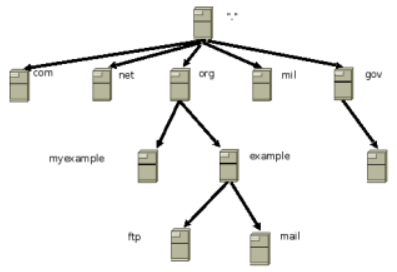
\includegraphics[width=0.8\textwidth]{assets/cap3/3.6.png}
\caption{Jerarquia y funcionamiento del DNS}
\label{fig:dns-jerarquia}
\end{figure}

\subsection{Componentes del DNS}

\begin{itemize}
    \item \textbf{Root Servers}: 13 servidores raiz (A--M), mayoria en USA.
    \item \textbf{TLD Servers}: servidores de dominio de nivel superior (.com, .es, etc.).
    \item \textbf{Authoritative DNS Servers}: servidores autoritativos para un dominio.
\end{itemize}

\subsection{Tipos de resolucion}

\begin{itemize}
    \item \textbf{Consulta interactiva}: el servidor consulta a otros y redirige al cliente.
    \item \textbf{Consulta recursiva}: el servidor resuelve completamente y devuelve la respuesta.
\end{itemize}

\subsection{DNS Internos vs Externos}

\begin{itemize}
    \item \textbf{DNS Interno}: resuelve nombres dentro de una red local (compania). Conoce IPs privadas.
    \item \textbf{DNS Externo / Autoritativo}: visible desde Internet. Solo contiene registros de servicios publicos.
    \item Los DNS autoritativos se configuran al registrar un dominio a traves de un \textbf{REGISTRAR} acreditado por \textbf{ICANN}.
\end{itemize}


\section{DHCP (Dynamic Host Configuration Protocol)}

El \textbf{DHCP} permite la administracion centralizada de la configuracion IP de los dispositivos de una red.

\begin{definicion}
\textbf{DHCP} (Dynamic Host Configuration Protocol) es un protocolo que asigna automaticamente direcciones IP y otros parametros de configuracion (mascara, gateway, DNS) a los dispositivos cuando se conectan a la red.
\end{definicion}

\subsection{Beneficios}

\begin{itemize}
    \item Administracion centralizada de configuracion IP.
    \item Configuracion consistente.
    \item Flexibilidad y escalabilidad.
\end{itemize}

\begin{figure}[H]
\centering
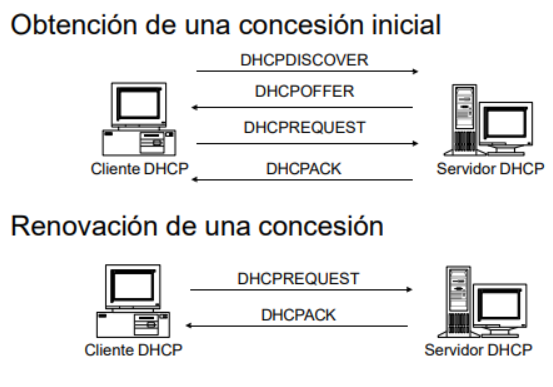
\includegraphics[width=0.8\textwidth]{assets/cap3/3.7.png}
\caption{Funcionamiento de DHCP: proceso DORA}
\label{fig:dhcp-dora}
\end{figure}

\subsection{Funcionamiento: concesion inicial (DORA)}

\begin{verbatim}
Cliente -> DHCPDISCOVER -> Servidor
Cliente <- DHCPOFFER    <- Servidor
Cliente -> DHCPREQUEST  -> Servidor
Cliente <- DHCPACK      <- Servidor
\end{verbatim}

\subsection{Renovacion}

\begin{verbatim}
Cliente -> DHCPREQUEST -> Servidor
Cliente <- DHCPACK     <- Servidor
\end{verbatim}

\subsection{Mensajes DHCP}

\begin{table}[htbp]
\centering
\small
\caption{Mensajes del protocolo DHCP}
\begin{tabularx}{\textwidth}{@{}lX@{}}
\toprule
\textbf{Mensaje} & \textbf{Significado} \\
\midrule
DHCPDISCOVER & El cliente pide una IP \\
DHCPOFFER & El servidor ofrece una concesion \\
DHCPREQUEST & El cliente solicita una concesion especifica \\
DHCPACK & El servidor confirma la concesion \\
DHCPDECLINE & El cliente rechaza la IP ofrecida \\
DHCPNACK & El servidor deniega la concesion \\
DHCPRELEASE & El cliente libera la concesion \\
DHCPINFORM & El cliente pide configuracion adicional \\
\bottomrule
\end{tabularx}
\end{table}

\subsection{Puertos}

\begin{itemize}
    \item Cliente: \textbf{UDP 68}
    \item Servidor: \textbf{UDP 67}
\end{itemize}

\subsection{Metodos de configuracion}

\begin{itemize}
    \item \textbf{Servidores DHCP}: asignan IPs automaticamente.
    \item \textbf{Agentes DHCP de relevo}: reenvian peticiones entre subredes.
    \item \textbf{BOOTP}: protocolo predecesor.
\end{itemize}

\subsection{Ambitos DHCP}

\begin{itemize}
    \item Definen rangos de direcciones IP asignables.
    \item Se pueden excluir direcciones manualmente (routers, firewalls, servidores).
    \item Se pueden crear superambitos combinando multiples ambitos.
\end{itemize}


\section{Practica 4: Cisco Packet Tracer}
\label{sec:practica4}

\subsection{Objetivos}

El objetivo de esta practica es entrar en contacto con el simulador de redes
Cisco Packet Tracer y comprender los conceptos fundamentales de una red de
area local:

\begin{enumerate}
    \item Configurar una red de area local (LAN) con al menos 3 ordenadores y un
    switch, asignando direcciones IP, mascara de subred y gateway.
    \item Verificar la comunicacion entre los ordenadores de la misma LAN
    mediante herramientas como ping.
    \item Crear una segunda LAN con un rango de direcciones diferente.
    \item Interconectar ambas LAN mediante un router, configurando sus interfaces
    de red para que actuen como gateway de cada LAN.
    \item Verificar que los ordenadores de una red pueden comunicarse con los de
    la otra a traves del router.
\end{enumerate}

\subsection{Material utilizado}

\begin{itemize}
    \item \textbf{Software}: Cisco Packet Tracer (simulador de redes Cisco).
    \item \textbf{Hardware simulado}: PCs personales, switches (conmutadores) y
    router (encaminador).
    \item \textbf{Redes}:
    \begin{itemize}
        \item Red 1: 192.168.10.0 / 255.255.255.0
        \item Red 2: 192.168.20.0 / 255.255.255.0
    \end{itemize}
\end{itemize}

\subsection{Desarrollo de la practica}

\subsubsection{Primera parte: configuracion de la LAN 192.168.10.0}

Se diseno una red local con 3 ordenadores personales y un switch. Cada
ordenador se configuro con los siguientes parametros:

\begin{itemize}
    \item \textbf{IP}: en el rango 192.168.10.0 (por ejemplo, 192.168.10.1,
    192.168.10.2, 192.168.10.3).
    \item \textbf{Mascara de subred}: 255.255.255.0 (/24).
    \item \textbf{Gateway}: 192.168.10.254 (direccion que ocupara el router).
\end{itemize}

Se anadieron etiquetas a los ordenadores para identificar su nombre y su
IP. A continuacion, se verifico la comunicacion entre los 3 ordenadores
mediante el comando \texttt{ping}. El resultado confirmo que todos los
ordenadores de la misma red local pueden comunicarse entre si a traves del
switch.

\begin{figure}[H]
\centering
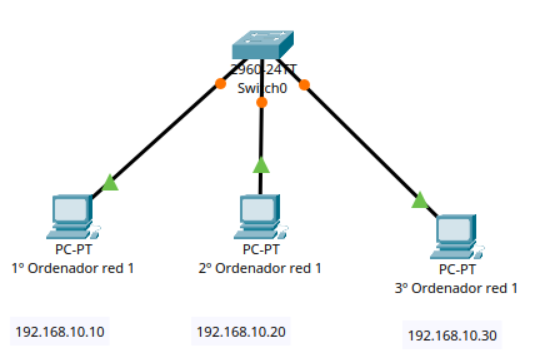
\includegraphics[width=0.8\textwidth]{assets/cap3/3.8.png}
\caption{Topologia de la primera LAN (192.168.10.0)}
\label{fig:lan1}
\end{figure}

\textbf{Comando de verificacion}:
\begin{lstlisting}[language=bash,caption={Verificacion de conectividad en la LAN 1},label={lst:ping-lan1}]
C:\> ping 192.168.10.2

Respuesta desde 192.168.10.2: bytes=32 tiempo<1ms TTL=128
Respuesta desde 192.168.10.2: bytes=32 tiempo<1ms TTL=128
Respuesta desde 192.168.10.2: bytes=32 tiempo<1ms TTL=128
\end{lstlisting}

\subsubsection{Segunda parte: configuracion de la LAN 192.168.20.0 e interconexion}

Se creo una segunda red local con 3 ordenadores mas y otro switch, esta vez
en el rango 192.168.20.0. La configuracion de cada ordenador fue:

\begin{itemize}
    \item \textbf{IP}: en el rango 192.168.20.0 (por ejemplo, 192.168.20.1,
    192.168.20.2, 192.168.20.3).
    \item \textbf{Mascara de subred}: 255.255.255.0.
    \item \textbf{Gateway}: 192.168.20.254.
\end{itemize}

Se verifico que los ordenadores de esta segunda LAN se comunicaban entre si.

\subsubsection{Tercera parte: conexion de ambas LAN mediante un router}

Para que los ordenadores de la red 192.168.10.0 puedan comunicarse con los de
la red 192.168.20.0, se anadio un \textbf{router} entre ambas redes. El router
cuenta con dos interfaces de red (tarjetas), una conectada a cada switch:

\begin{itemize}
    \item \textbf{Interfaz 1}: IP 192.168.10.254 / Mascara 255.255.255.0
    (conectada al switch de la LAN 1).
    \item \textbf{Interfaz 2}: IP 192.168.20.254 / Mascara 255.255.255.0
    (conectada al switch de la LAN 2).
\end{itemize}

Estas dos direcciones son las \textbf{puertas de enlace} (gateway) de cada red.

Se etiquetaron las conexiones del router indicando la red a la que se
conecta cada interfaz y la IP configurada. Finalmente, se verifico la
comunicacion entre ordenadores de ambas redes:

\begin{lstlisting}[language=bash,caption={Verificacion de conectividad entre redes},label={lst:ping-interred}]
C:\> ping 192.168.20.2

Respuesta desde 192.168.20.2: bytes=32 tiempo=1ms TTL=127
Respuesta desde 192.168.20.2: bytes=32 tiempo=1ms TTL=127
Respuesta desde 192.168.20.2: bytes=32 tiempo=1ms TTL=127
\end{lstlisting}

\begin{figure}[H]
\centering
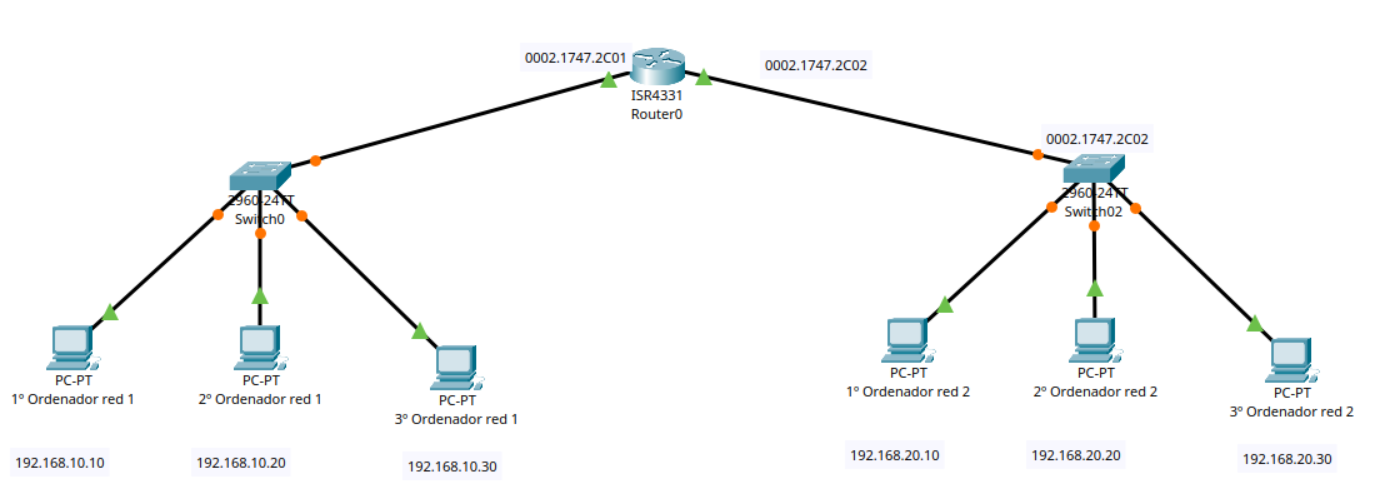
\includegraphics[width=0.8\textwidth]{assets/cap3/3.9.png}
\caption{Topologia completa: interconexion de dos LAN mediante un router}
\label{fig:topologia-completa}
\end{figure}

\subsection{Analisis de la comunicacion entre redes}

Cuando el PC 192.168.10.1 envia un \texttt{ping} al PC 192.168.20.2, ocurre lo
siguiente:

\begin{enumerate}
    \item El PC 192.168.10.1 calcula la red destino aplicando su mascara a la
    IP 192.168.20.2. Detecta que la red destino (192.168.20.0) no coincide
    con su propia red (192.168.10.0).
    \item Por tanto, no puede enviar el paquete directamente. Lo envia a su
    \textbf{gateway}: 192.168.10.254.
    \item El router recibe el paquete por su interfaz 192.168.10.254. Consulta
    su tabla de encaminamiento y detecta que la red 192.168.20.0 es
    \textbf{directamente conectada} a traves de su otra interfaz.
    \item El router reenvia el paquete por la interfaz 192.168.20.254 hacia el
    switch de la LAN 2.
    \item El switch entrega el paquete al PC 192.168.20.2.
    \item El PC 192.168.20.2 responde. Como la IP 192.168.10.1 pertenece a otra
    red, el PC 192.168.20.2 envia la respuesta a su gateway (192.168.20.254).
    \item El router reenvia la respuesta por la interfaz 192.168.10.254.
\end{enumerate}

Este proceso ilustra el concepto fundamental de \textbf{inter-networking}: la
interconexion de redes distintas mediante un dispositivo de capa 3 (router).

\subsection{Relacion teoria-practica}

\begin{table}[htbp]
\centering
\small
\caption{Conexion entre conceptos teoricos y elementos de la Practica 4}
\begin{tabularx}{\textwidth}{@{}lX@{}}
\toprule
\textbf{Concepto teorico} & \textbf{Observacion/aplicacion en la practica} \\
\midrule
Red de computadores & Se disenaron dos redes locales con 3 ordenadores cada una, switch y enlaces fisicos \\
Switch (Capa 2) & Conecta los 3 ordenadores de cada LAN y reenvia paquetes al destinatario correcto \\
Router (Capa 3) & Interconecta las dos LAN distintas, encaminando paquetes entre 192.168.10.0 y 192.168.20.0 \\
Direccion IP & Cada ordenador tiene una IP unica dentro de su rango (192.168.10.x o 192.168.20.x) \\
Mascara de subred & 255.255.255.0 indica que los primeros 3 octetos son red y el ultimo es host \\
Gateway & 192.168.10.254 y 192.168.20.254 son las interfaces del router que actuan como puerta de enlace \\
Comunicacion intra-red & Los PCs de la misma LAN se comunican directamente a traves del switch (ping funciona) \\
Comunicacion inter-red & Los PCs de distintas redes necesitan el router; el ping inter-red confirma el encaminamiento \\
Tabla de encaminamiento & El router internamente tiene una entrada indicando que ambas redes son directamente conectadas \\
Modelo TCP/IP (Capa 3) & El ICMP (ping) opera sobre IP, demostrando la funcion de la capa de red \\
\bottomrule
\end{tabularx}
\end{table}


\section{Resumen de la Unidad 3}

\begin{itemize}
    \item El \textbf{modelo TCP/IP} organiza la comunicacion en cuatro capas: aplicacion, transporte, internet y enlace.
    \item \textbf{TCP} es un protocolo de transporte orientado a conexion y fiable; \textbf{UDP} es un protocolo sin conexion y mas rapido, adecuado para aplicaciones en tiempo real.
    \item Cada dispositivo en una red tiene una \textbf{direccion IP} unica de 32 bits (IPv4), representada en notacion decimal punteada. Puede ser \textbf{dinamica} (asignada por DHCP) o \textbf{fija}.
    \item El \textbf{direccionamiento con clase} (A, B, C, D, E) permite asignar rangos de direcciones segun el tamano de la red. Las \textbf{direcciones privadas} (10.0.0.0/8, 172.16.0.0/12, 192.168.0.0/16) se usan en redes locales.
    \item \textbf{CIDR} reemplazo el direccionamiento por clases mediante notacion de prefijo (ej. /24), permitiendo crear redes de cualquier tamano y agregar rutas (supernetting).
    \item El \textbf{DNS} traduce nombres de dominio a direcciones IP mediante una estructura jerarquica de servidores raiz, TLD y autoritativos.
    \item \textbf{DHCP} asigna automaticamente direcciones IP y configuracion de red a los dispositivos mediante el proceso DORA (Discover, Offer, Request, Acknowledge).
    \item La \textbf{Practica 4} aplica estos conceptos simulando dos LAN conectadas mediante un router en Cisco Packet Tracer, configurando IPs, mascaras, gateways y verificando conectividad con ping.
\end{itemize}

%%%%%%%%%%%%%%%%%%%%%%%%%%%%%%%%%%%%%%%%%%%%%%%%%%%%%%%%%%%%%%%%%%%%%%%%%%%%%%%
%                         CAPITULO 4
%           Introduccion a las Redes Industriales
%%%%%%%%%%%%%%%%%%%%%%%%%%%%%%%%%%%%%%%%%%%%%%%%%%%%%%%%%%%%%%%%%%%%%%%%%%%%%%%

\chapter{Introduccion a las Redes Industriales}

Hasta ahora hemos estudiado como comunican dispositivos mediante cables, ondas
de radio, y como se organizan las redes de computadores mediante direcciones IP,
switches y routers. Sin embargo, en un entorno de fabricacion o produccion, las
redes no solo conectan ordenadores: conectan sensores, actuadores, robots, PLCs
y sistemas de supervision, todo trabajando en tiempo real para controlar procesos
industriales.

En este capitulo introducimos el concepto de \textbf{redes industriales}, tambien
conocidas como redes de comunicacion para la automatizacion y control de
procesos. Veremos que son, como funcionan, que tipos existen y por que son
fundamentales en la industria moderna.


\section{Sistemas industriales distribuidos}

\subsection{Definicion}

Un \textbf{sistema industrial distribuido} es una arquitectura de control y
automatizacion donde multiples dispositivos, sensores, actuadores y sistemas
informaticos estan interconectados para operar de manera descentralizada.

\begin{definicion}{Sistema industrial distribuido}
Un \textbf{sistema industrial distribuido} es una arquitectura de control donde
multiples dispositivos (PLCs, sensores, actuadores, robots) comparten la
responsabilidad de la operacion, interconectados mediante una red de
comunicacion industrial. Ofrece mayor flexibilidad, escalabilidad y eficiencia
que los sistemas centralizados tradicionales.
\end{definicion}

En un sistema centralizado clasico, un unico controlador (PLC o computador)
toma todas las decisiones y envia ordenes a los dispositivos de campo. En un
sistema distribuido, la inteligencia se reparte: cada dispositivo puede tomar
decisiones locales y compartir informacion con el resto.

\subsection{Caracteristicas principales}

Los sistemas industriales distribuidos se caracterizan por:

\begin{itemize}
    \item \textbf{Descentralizacion}: multiples dispositivos comparten la
    responsabilidad de la operacion. No hay un unico punto de control.
    \item \textbf{Interconectividad}: se basan en redes de comunicacion industrial
    como Ethernet/IP, Modbus, Profibus o IoT industrial.
    \item \textbf{Escalabilidad}: se pueden agregar nuevos dispositivos sin afectar
    la operacion global.
    \item \textbf{Tolerancia a fallos}: al no depender de un unico nodo, el sistema
    puede seguir funcionando ante fallos parciales.
    \item \textbf{Optimizacion de recursos}: permite un uso eficiente de energia,
    maquinaria y mano de obra.
    \item \textbf{Automatizacion avanzada}: utiliza PLCs, SCADA, IIoT e inteligencia
    artificial.
\end{itemize}

\subsection{Aplicaciones y ventajas}

Las aplicaciones mas comunes incluyen:
\begin{itemize}
    \item \textbf{Automatizacion de fabricas}: produccion y ensamblaje de productos.
    \item \textbf{Redes de energia inteligente (Smart Grid)}: gestion eficiente de
    energia electrica.
    \item \textbf{Transporte y logistica}: control distribuido en almacenes y vehiculos
    autonomos.
    \item \textbf{Industria 4.0}: implementacion de IoT y Big Data para optimizacion.
    \item \textbf{Robotica industrial}: control distribuido en lineas de produccion.
\end{itemize}

Las ventajas principales son: mayor eficiencia operativa, reduccion de costes de
mantenimiento, mayor adaptabilidad a cambios en la produccion, y mejora en la
recopilacion y analisis de datos.


\section{Redes industriales: conceptos fundamentales}

\subsection{Definicion}

\begin{definicion}{Red industrial}
Una \textbf{red industrial} es una estructura de comunicacion automatizada que
gestiona procesos industriales, involucrando actuadores, computadoras, maquinas,
sensores, interfaces, medios de comunicacion (fibra optica, cables, redes
inalambricas) y robots. Su objetivo es transmitir y compartir datos para garantizar
un funcionamiento eficiente de los procesos productivos.
\end{definicion}

\subsection{Como funcionan}

Las redes industriales reemplazan el modelo tradicional de control cableado a
mano (donde cada dispositivo necesitaba su propio cable de control) por un modelo
de comunicacion digital donde multiples dispositivos comparten un unico medio de
transmision.

Este modelo reduce drasticamente la cantidad de cableado necesario, simplifica
la organizacion del sistema y permite una flexibilidad mucho mayor para
reconfigurar la produccion.

\subsection{Convergencia de TI y TO (OT)}

En la industria moderna se distinguen dos tecnologias:

\begin{itemize}
    \item \textbf{TI (Tecnologia de la Informacion)}: se ocupa de la entrega de
    informacion cuando un profesional la solicita. Sistemas de datos, ERP, CRM.
    \item \textbf{TO (Tecnologia Operacional) o OT}: trabaja con la entrega de
    informacion en un momento especifico bajo una condicion determinada.
    Controla equipos industriales en tiempo real.
\end{itemize}

La convergencia de TI y TO esta relacionada con el auge del \textbf{edge computing}
(computacion en el borde): trasladar los recursos informaticos a la ubicacion
fisica de la fuente de datos (por ejemplo, en la propia fabrica), permitiendo unificar
sistemas que tradicionalmente estaban aislados.

\subsection{Desafios}

Las redes industriales enfrentan desafios especificos:
\begin{itemize}
    \item \textbf{Complejidad en la integracion}: sistemas heterogeneos de diferentes
    fabricantes deben comunicarse.
    \item \textbf{Ciberseguridad}: las redes industriales son objetivos criticos; un ataque
    puede parar la produccion.
    \item \textbf{Capacitacion especializada}: requiere personal con conocimientos en
    automatizacion y redes.
\end{itemize}


\section{Clasificacion de las redes industriales}

Las redes industriales se clasifican segun el nivel de la piramide de automatizacion:

\begin{table}[htbp]
\centering
\small
\caption{Niveles de las redes industriales}
\begin{tabularx}{\textwidth}{@{}l>{\raggedright\arraybackslash}X>{\raggedright\arraybackslash}X@{}}
\toprule
\textbf{Nivel} & \textbf{Funcion} & \textbf{Ejemplos} \\
\midrule
Nivel de informacion (gestion) & Planificacion, ERP, MES & Redes Ethernet, TCP/IP, bases de datos \\
Nivel de control & Controladores, PLCs, SCADA & ControlNet, Ethernet/IP \\
Nivel de campo y proceso & Sensores, actuadores, transmisores & Profibus, Modbus, CAN \\
Nivel de entrada/salida & Dispositivos simples, fotocelulas & AS-i, Sensor Bus \\
\bottomrule
\end{tabularx}
\end{table}

\subsection{Clasificacion por funcionalidad}

Segun sus capacidades y el tipo de datos que transportan:

\begin{enumerate}
    \item \textbf{Sensor Bus (buses de sensores)}: conectan sensores digitales y
    actuadores simples. Transmite pocos datos, distancias cortas, bajo costo.
    Ejemplos: AS-i, CAN, Interbus.
    \item \textbf{Device Bus (buses de dispositivos)}: intermedian entre sensores y
    PLCs. Manejan variables de proceso (presion, temperatura, flujo).
    Alcance hasta 500 metros. Ejemplos: Modbus, Profibus DP, DeviceNet.
    \item \textbf{Field Bus (buses de campo)}: permiten que varios instrumentos se
    comuniquen en red para control y monitoreo. Conectan mas equipos a mayor
    distancia. Ejemplos: Foundation Fieldbus, Profibus PA.
    \item \textbf{Control Bus / Ethernet Industrial}: redes de alta velocidad para
    control en tiempo real. Ejemplos: Ethernet/IP, PROFINET, EtherCAT, ControlNet.
\end{enumerate}

\subsection{Tabla comparativa de tipos de redes industriales}

\begin{table}[htbp]
\centering
\small
\caption{Comparacion de tipos de redes industriales}
\begin{tabularx}{\textwidth}{@{}l>{\raggedright\arraybackslash}X>{\raggedright\arraybackslash}X>{\raggedright\arraybackslash}X@{}}
\toprule
\textbf{Tipo} & \textbf{Velocidad} & \textbf{Funcionalidad} & \textbf{Uso tipico} \\
\midrule
Sensor Bus & Baja & Simple & Sensores, actuadores binarios \\
Device Bus & Media & Media & Transmisores, servomotores \\
Field Bus & Media & Alta & Control de procesos continuos \\
Ethernet Industrial & Alta & Muy alta & Control en tiempo real, integracion TI/TO \\
\bottomrule
\end{tabularx}
\end{table}


\section{Principales protocolos de redes industriales}

\subsection{PROFINET}

PROFINET es una solucion de Ethernet Industrial abierta basada en estandares
internacionales. Es el protocolo de comunicacion desarrollado para intercambiar
datos entre controladores y dispositivos en un sector automatizado.

Utiliza Ethernet estandar como medio de comunicacion, lo que permite que otros
protocolos Ethernet (SNMP, MQTT, HTTP) coexistan en la misma infraestructura.
Ademas, define la comunicacion ciclica y aciclica entre componentes, incluyendo
diagnosticos, seguridad funcional, alarmas e informacion adicional.

\subsection{PROFIBUS}

PROFIBUS es una red digital que proporciona comunicacion entre sensores de
campo y controladores. Surgio inicialmente como PROFIBUS FMS (Fieldbus Message
Specification), pero hoy en dia los mas utilizados son:

\begin{itemize}
    \item \textbf{PROFIBUS DP} (Decentralised Peripherals): para automatizacion de
    fabricas, comunicacion rapida entre PLCs y dispositivos de campo.
    \item \textbf{PROFIBUS PA} (Process Automation): para procesos continuos como
    industrias petroquimica y minera.
\end{itemize}

\subsection{EtherCAT}

EtherCAT (Ethernet for Control Automation Technology) es un protocolo que lleva
la potencia y flexibilidad de Ethernet a la automatiz industrial, al control de
movimientos y a los sistemas de control en tiempo real.

Fue desarrollado por Beckhoff Automation y estandarizado bajo IEC 61158. Es
mantenido por el EtherCAT Technology Group (ETG). Su principal ventaja es la
extremada velocidad de transmision y la sincronizacion precisa de los dispositivos.

\subsection{ControlNet}

ControlNet utiliza el Protocolo Industrial Comun (CIP) para las capas superiores
del modelo OSI. Se desarrollo para ofrecer control confiable y de alta velocidad,
con transferencia de datos I/O programada en momentos especificos.

Garantiza que los mensajes criticos que no dependen del tiempo se ejecuten sin
interferir en la transferencia de datos de control. Se utiliza normalmente para
aplicaciones redundantes.

\subsection{Ethernet en la industria: importancia en la Industria 4.0}

Ethernet se ha convertido en el estandar mundial para la intercomunicacion de
datos en red porque:
\begin{itemize}
    \item Tiene una implementacion simple y costos reducidos.
    \item Permite el uso de varios protocolos en un entorno industrial.
    \item Es interoperable y escalable para las demandas.
    \item Sigue en constante evolucion y mejora.
\end{itemize}

En la \textbf{Industria 4.0}, la informacion fluye horizontal y verticalmente a traves
de toda la organizacion. Esto requiere una infraestructura de comunicacion que
abarque todas las maquinas, computadoras, robots y equipos, lo cual solo es
posible con Ethernet e Internet unidos al IIoT (Internet Industrial de las Cosas).


\section{Resumen de la Unidad 5}

\begin{itemize}
    \item Los \textbf{sistemas industriales distribuidos} descentralizan el control,
    permitiendo que multiples dispositivos compartan la responsabilidad de la
    operacion y mejoren la tolerancia a fallos.
    \item Una \textbf{red industrial} es una estructura de comunicacion que gestiona
    procesos industriales, conectando sensores, actuadores, PLCs, robots y
    sistemas de supervision.
    \item La \textbf{convergencia de TI y TO} (OT) unifica los sistemas de informacion
    empresarial con los sistemas de control en tiempo real, facilitando el
    \textbf{edge computing} y la Industria 4.0.
    \item Las redes industriales se clasifican en niveles: informacion, control,
    campo y E/S. Por funcionalidad: Sensor Bus, Device Bus, Field Bus y
    Ethernet Industrial.
    \item Los principales protocolos son: \textbf{PROFINET}, \textbf{PROFIBUS},
    \textbf{EtherCAT}, \textbf{ControlNet}, \textbf{Modbus}, \textbf{Ethernet/IP}.
    \item \textbf{Ethernet} es el estandar dominante en la industria moderna por su
    simplicidad, bajo costo, interoperabilidad y capacidad para soportar
    multiples protocolos simultaneamente.
\end{itemize}

%%%%%%%%%%%%%%%%%%%%%%%%%%%%%%%%%%%%%%%%%%%%%%%%%%%%%%%%%%%%%%%%%%%%%%%%%%%%%%%
%                         CAPITULO 5
%                  Unidad 5: Encaminadores y Routing
%%%%%%%%%%%%%%%%%%%%%%%%%%%%%%%%%%%%%%%%%%%%%%%%%%%%%%%%%%%%%%%%%%%%%%%%%%%%%%%

\chapter{Encaminadores y Protocolos de Routing}

En los capitulos anteriores hemos visto como los dispositivos se conectan en
redes, como se comunican mediante direcciones IP y como los switches operan
en la capa de enlace. Sin embargo, cuando una red crece y se divide en multiples
subredes, surge un problema fundamental: como hacer que los paquetes de datos
lleguen desde una red a otra, eligiendo el mejor camino posible.

En este capitulo estudiamos el \textbf{encaminamiento} (routing): el proceso de
tomar decisiones sobre por donde enviar los paquetes en una red interconectada.
Veremos los fundamentos teoricos, los algoritmos que permiten calcular caminos
optimos, y los protocolos que permiten a los routers compartir informacion de
rutas automaticamente.


\section{Conceptos fundamentales de encaminamiento}

\begin{definicion}{Encaminamiento y conmutacion}
El \textbf{encaminamiento} (routing) es el proceso de eleccion del camino optimo
que debe seguir un paquete desde su origen hasta su destino a traves de una
red interconectada. Es una decision de control.

La \textbf{conmutacion} (switching) es el acto de retransmitir los datos por uno de
los caminos posibles, una vez tomada la decision. Es una accion de reenvio.
\end{definicion}

El encaminamiento toma la decision sobre el camino a seguir; la conmutacion
ejecuta esa decision reenviando el paquete por la interfaz correspondiente.

\subsection{Tipos de encaminamiento}

Existen varias estrategias para encaminar paquetes:

\begin{itemize}
    \item \textbf{Difusion (Broadcasting)}: envio de informacion a todos los nodos de la
    red. Se implementa mediante \textbf{inundacion} (flooding): cada nodo reenvia el
    paquete a todos sus vecinos excepto al que se lo envio.
    \begin{itemize}
        \item Ventaja: muy robusta, garantiza que se prueban todos los caminos posibles.
        \item Desventaja: mucha sobrecarga, transmisiones y recepciones innecesarias.
    \end{itemize}
    \item \textbf{Camino mas corto (Shortest Path)}: una de las estrategias mas empleadas.
    Se minimiza el numero de saltos entre origen y destino. De manera generica,
    se puede hablar de \textbf{coste} o \textbf{metrica}, estableciendo alguna medida como
    distancia, retardo, ancho de banda, etc.
    \item \textbf{Encaminamiento optimo}: el camino mas corto no siempre ofrece el mejor
    comportamiento (por ejemplo, puede estar congestionado). El encaminamiento
    optimo busca la mejor ruta segun multiples criterios mediante optimizacion
    matematica.
    \item \textbf{Patata caliente (Hot Potato)}: un nodo manda cada paquete por la interfaz
    menos cargada, deshaciendose del mismo lo antes posible. Es una tecnica muy
    simple que no considera la distancia global.
\end{itemize}


\section{Grafos y encaminamiento}

Los \textbf{grafos} son una herramienta matematica que se emplea para formular
problemas de encaminamiento.

\begin{definicion}{Grafo}
Un \textbf{grafo} es una estructura matematica definida como G = (N, d), donde:
\begin{itemize}
    \item \textbf{N} es un conjunto de nodos (vertices).
    \item \textbf{d} es una coleccion de enlaces (edges), donde cada enlace consta de un
    par de nodos de N.
\end{itemize}
\end{definicion}

Al trasladar un grafo a un problema de encaminamiento:
\begin{itemize}
    \item Los \textbf{nodos} N son los encaminadores (routers) de la red.
    \item Los \textbf{enlaces} d se corresponden con los enlaces fisicos entre ellos.
\end{itemize}

\subsection{Tipos de grafos}

\begin{itemize}
    \item \textbf{Grafos dirigidos}: los enlaces son pares ordenados (u,v) donde el
    orden importa. (u,v) $\neq$ (v,u).
    \item \textbf{Grafos no dirigidos}: los enlaces no tienen direccion. (u,v) = (v,u).
\end{itemize}

\subsection{Concatenaciones de enlaces}

\begin{itemize}
    \item \textbf{Paseo (Walk)}: secuencia de nodos (n1, n2, ..., nl) tal que cada pareja
    (ni-1, ni) es un enlace del grafo.
    \item \textbf{Camino (Path)}: es un paseo en el que no hay nodos repetidos.
    \item \textbf{Ciclo o bucle (Cycle)}: camino con mas de un enlace en el que el nodo
    inicial coincide con el final (n1 = nl).
\end{itemize}

\subsection{Grafo conectado}

Se dice que un grafo esta \textbf{conectado} si cualquier par de nodos esta conectado
por un camino. En redes de comunicaciones, esto significa que cualquier router
puede comunicarse con cualquier otro.

\subsection{Representacion de grafos}

Los grafos se pueden representar de dos formas principales:

\begin{table}[htbp]
\centering
\small
\caption{Representacion de grafos}
\begin{tabularx}{\textwidth}{@{}l>{\raggedright\arraybackslash}X>{\raggedright\arraybackslash}X@{}}
\toprule
\textbf{Aspecto} & \textbf{Lista de adyacencia} & \textbf{Matriz de adyacencia} \\
\midrule
Estructura & Array de N listas, una por nodo, con punteros a vecinos & Matriz F de dimension N x N \\
Memoria & Menor memoria, apropiada para grafos dispersos (sparse) & Mayor memoria, N\^{}2 elementos \\
Ventajas & Eficiente en memoria para grafos con pocos enlaces & Busqueda muy rapida, facil asignar costes \\
Desventajas & Busqueda puede ser lenta & Requiere mas memoria, se usa en grafos pequenos \\
Grafos no dirigidos & Numero de punteros = 2|d| & Matriz simetrica: F\^{}T = F \\
Grafos dirigidos & Numero de punteros = |d| & Matriz no simetrica \\
\bottomrule
\end{tabularx}
\end{table}

\subsection{Costes en los enlaces}

En algunas ocasiones se asignan \textbf{costes} c(u,v) a los enlaces, representando
metricas como:
\begin{itemize}
    \item Distancia fisica (kilometros).
    \item Retardo (milisegundos).
    \item Ancho de banda (Mbps).
    \item Congestion actual.
\end{itemize}

El objetivo del encaminamiento es entonces encontrar el camino con menor coste
acumulado.


\section{Algoritmos de camino mas corto}

La idea principal es encontrar el camino con un coste minimo entre una fuente
(S) y un destino (D). Si c(u,v) se mantiene constante para todos los enlaces,
la solucion es la ruta de menor numero de saltos.

\subsection{Algoritmos con una unica fuente}

Encuentran el camino mas corto entre un nodo origen S y el resto de nodos:

\begin{itemize}
    \item \textbf{Dijkstra}: funciona con grafos donde los costes son positivos.
    Es el algoritmo mas utilizado en protocolos como OSPF.
    \item \textbf{Bellman-Ford}: permite costes negativos (si no hay ciclos negativos).
    Es la base del encaminamiento por vectores de distancia (RIP).
\end{itemize}

\subsection{Algoritmos para toda la red}

Encuentran el camino mas corto entre todas las posibles parejas de nodos:

\begin{itemize}
    \item \textbf{Floyd-Warshall}: algoritmo de programacion dinamica.
    \item \textbf{Johnson}: combina Dijkstra y Bellman-Ford para grafos dispersos.
\end{itemize}

\subsection{Arbol de expansion minimo (Minimum Spanning Tree)}

Un \textbf{arbol} es un grafo no dirigido, conectado y sin ciclos. El numero de
enlaces es igual al numero de nodos menos 1: |d| = |N| - 1.

Un \textbf{Spanning Tree} cubre (se expande por) todos los nodos de un grafo. El
\textbf{Minimum Spanning Tree (MST)} es aquel que tiene el menor coste total.

\textbf{Aplicaciones}:
\begin{itemize}
    \item Procesos de difusion (broadcast) de informacion.
    \item Redes de area local: bridges (IEEE 802.1D) emplean el MST para eliminar
    enlaces no necesarios y evitar bucles.
\end{itemize}

\textbf{Algoritmos}: Kruskal y Prim.


\section{Protocolos de encaminamiento}

Los nodos (encaminadores) toman decisiones en base a cierta informacion. Es
necesario disponer de un \textbf{protocolo de senalizacion} que proporcione un metodo
para transportar dicha informacion por la red.

\subsection{Clasificacion de protocolos}

\begin{table}[htbp]
\centering
\small
\caption{Clasificacion de protocolos de encaminamiento}
\begin{tabularx}{\textwidth}{@{}l>{\raggedright\arraybackslash}X@{}}
\toprule
\textbf{Tipo} & \textbf{Descripcion} \\
\midrule
Vector de distancia (DV) & Cada router intercambia periodicamente su tabla con los vecinos. Usa Bellman-Ford. Ejemplo: RIP. \\
Estado de enlace (LS) & Cada router difunde el estado de sus enlaces a toda la red. Usa Dijkstra. Ejemplo: OSPF. \\
\bottomrule
\end{tabularx}
\end{table}

\subsection{Encaminamiento por vector de distancia}

Se basa en el algoritmo de Bellman-Ford. Cada nodo de la red mantiene una tabla
de encaminamiento con una entrada por cada uno del resto de nodos:

\begin{itemize}
    \item \textbf{Distancia}: metrica o coste del camino hacia dicho nodo.
    \item \textbf{Interfaz de salida}: necesaria para alcanzarle.
\end{itemize}

Periodicamente, cada nodo intercambia la informacion de su tabla con sus vecinos.

\textbf{Problemas}:
\begin{itemize}
    \item \textbf{Convergencia lenta}: los cambios en la topologia tardan en propagarse.
    \item \textbf{Propagacion rapida de ``buenas noticias'' y lenta de las ``malas''}:
    cuando un enlace mejora, la noticia se propaga rapido; cuando empeora, tarda.
    \item \textbf{Count-to-infinity}: si un enlace cae, los routers pueden incrementar
    sus metricas hasta el infinito de forma ciclica.
\end{itemize}

\textbf{Soluciones al count-to-infinity}:
\begin{itemize}
    \item \textbf{Limitar el infinito}: en RIP, el limite es 16 saltos (una red a 16
    saltos se considera inalcanzable).
    \item \textbf{Horizonte dividido (Split Horizon)}: un router no anuncia una ruta
    de regreso a la interfaz por la que la aprendio.
    \item \textbf{Horizonte dividido con respuesta envenenada (Poison Reverse)}: si
    se anuncia la ruta de regreso, se hace con distancia infinita.
    \item \textbf{Actualizaciones forzadas (Triggered Updates)}: cuando un router detecta
    un cambio, difunde inmediatamente la informacion sin esperar al temporizador.
\end{itemize}

\subsection{Encaminamiento por estado de enlace}

\textbf{Desventajas}:
\begin{itemize}
    \item Necesidad de informacion global sobre la red.
    \item Envio de un numero mayor de mensajes: sobrecarga.
    \item Un evento de cambio en la topologia debe notificarse a todos los nodos.
\end{itemize}

\textbf{Protocolo OSPF} (Open Shortest Path First):
\begin{itemize}
    \item Definido en el RFC 2328 (version 2).
    \item Es un protocolo Intra-AS (dentro de un Sistema Autonomo).
    \item Utiliza el algoritmo de Dijkstra.
    \item Cada router conoce la topologia completa de la red.
\end{itemize}

\subsection{Encaminamiento jerarquico: Sistemas Autonomos (AS)}

Internet esta organizada en \textbf{Sistemas Autonomos} (AS):

\begin{definicion}{Sistema Autonomo (AS)}
Un \textbf{Sistema Autonomo (AS)} es una coleccion de redes y encaminadores
gestionadas y administradas por una misma autoridad (por ejemplo, un ISP, una
universidad, una empresa).
\end{definicion}

\begin{itemize}
    \item \textbf{Encaminadores internos del AS}: interconectan redes dentro del
    propio AS. Solo conocen en detalle la organizacion local. Utilizan protocolos
    \textbf{IGP} (Interior Gateway Protocol).
    \item \textbf{Encaminadores externos o frontera (border router)}: interconectan
    varios sistemas autonomos. Conocen el camino al resto de AS, pero no en
    detalle. Utilizan protocolos \textbf{EGP} (Exterior Gateway Protocol).
\end{itemize}

\textbf{Protocolos IGP} (dentro de un AS):
\begin{itemize}
    \item \textbf{RIP}: Routing Information Protocol.
    \item \textbf{OSPF}: Open Shortest Path First.
    \item \textbf{IGRP}: Internal Gateway Routing Protocol (de Cisco).
\end{itemize}

\textbf{Protocolos EGP} (entre AS):
\begin{itemize}
    \item \textbf{BGP}: Border Gateway Protocol. Es el protocolo que sostiene Internet,
    permitiendo que los diferentes AS intercambien informacion de rutas.
\end{itemize}


\section{Protocolo RIP (Routing Information Protocol)}

\subsection{Caracteristicas generales}

RIP es un protocolo de encaminamiento interior (IGP) basado en vectores de
distancia (algoritmo Bellman-Ford).

\begin{table}[htbp]
\centering
\small
\caption{Versiones de RIP}
\begin{tabularx}{\textwidth}{@{}l>{\raggedright\arraybackslash}X@{}}
\toprule
\textbf{Version} & \textbf{Caracteristicas} \\
\midrule
RIP v1 (RFC 1058, 1993) & No soporta VLSM/CIDR, envia broadcast \\
RIP v2 (RFC 2453, 1998) & Soporta VLSM/CIDR, envia multicast, incluye mascara \\
RIPng (RFC 2080, 1997) & Version para IPv6, puerto UDP 521, multicast FF02::9 \\
\bottomrule
\end{tabularx}
\end{table}

Los vectores de distancia incluyen:
\begin{itemize}
    \item La lista de destinos (redes) alcanzables por cada router.
    \item La distancia (numero de saltos) a dichos destinos.
\end{itemize}

La metrica de RIP es el \textbf{numero de saltos}. El limite de infinito es 16 saltos.
RIP utiliza los puertos UDP 520 (RIPv2) y 521 (RIPng).

\subsection{Temporizadores de RIP}

RIP utiliza tres temporizadores principales:

\begin{itemize}
    \item \textbf{Temporizador periodico} (25-35 s): intervalo de envio de mensajes
    RESPONSE para anunciar vectores de distancia. El valor oficial es 30 s, pero
    en la practica se usa un valor aleatorio entre 25 y 35 s para evitar
    sincronizacion.
    \item \textbf{Temporizador de expiracion} (180 s): controla el periodo de validez
    de una entrada. Si no se recibe actualizacion durante 180 s (equivalente a
    3 intervalos periodicos), la entrada deja de considerarse valida.
    \item \textbf{Temporizador de ``coleccion de basura''} (120 s): cuando una entrada
    expira, no se elimina inmediatamente. Se sigue anunciando con metrica 16
    (destino inalcanzable) durante 120 s adicionales para notificar a los vecinos.
\end{itemize}

\subsection{Mensajes RIP}

\begin{itemize}
    \item \textbf{REQUEST}: enviados por un router cuando se conecta a la red, o cuando
    caduca una entrada.
    \item \textbf{RESPONSE}: enviados periodicamente con los vectores de distancia, en
    respuesta a una solicitud, o como actualizacion forzada cuando cambia la
    distancia a una red.
\end{itemize}

\subsection{RIPng para IPv6}

RIPng (RIP new generation) es la adaptacion de RIP-2 para IPv6:
\begin{itemize}
    \item Los mensajes se encapsulan en datagramas UDP dirigidos al puerto 521.
    \item Se difunden a la direccion IPv6 multicast FF02::9.
    \item Los vectores de distancia anuncian prefijos de red IPv6 en lugar de
    direcciones IPv4.
    \item No incluye el campo ``Next Hop'' en cada entrada (se usa un mecanismo
    separado).
    \item No utiliza autenticacion propia; delega a los mecanismos de IPv6.
\end{itemize}


\section{Tablas de Encaminamiento}

\subsection{Encaminamiento ``Next-Hop''}

\begin{definicion}
El principio de encaminamiento \textbf{Next-Hop} se basa en la optimizacion: si el camino mas corto entre A y D pasa por B, entonces el camino mas corto de B a D es la misma ruta. Por tanto, solo se necesita conocer el \textbf{siguiente encaminador inmediato} (next hop), no la ruta completa.
\end{definicion}

\begin{figure}[H]
\centering
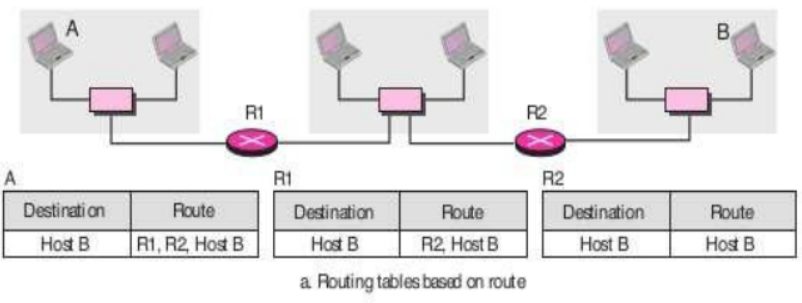
\includegraphics[width=0.8\textwidth]{assets/cap5/5.1.png}
\caption{Principio de encaminamiento next-hop}
\label{fig:next-hop}
\end{figure}

\subsection{Estructura de una tabla de encaminamiento}

Una tabla de encaminamiento contiene las siguientes entradas:

\begin{itemize}
    \item \textbf{Destino}: red o host de destino.
    \item \textbf{Mascara o prefijo de red (CIDR)}: define la porcion de red de la direccion.
    \item \textbf{Siguiente salto (next hop)}: direccion del siguiente router hacia el destino.
    \item \textbf{Coste}: metrica asociada al camino.
\end{itemize}

Tipos de entrada destino:
\begin{itemize}
    \item \textbf{Host especifico}: no viable en Internet por el gran numero de equipos.
    \item \textbf{Red}: con prefijo CIDR, la entrada mas utilizada.
    \item \textbf{Default}: para paquetes sin coincidencia en las demas entradas.
\end{itemize}

\begin{figure}[H]
\centering
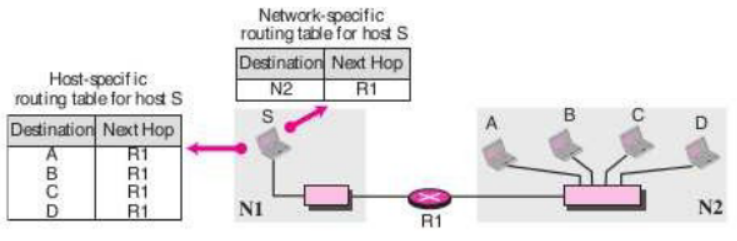
\includegraphics[width=0.8\textwidth]{assets/cap5/5.2.png}
\caption{Ejemplo de tabla de encaminamiento}
\label{fig:tabla-encaminamiento}
\end{figure}

\subsection{Ejemplo practico}

Dada una topologia de red con varios routers:
\begin{enumerate}
    \item Determinar la tabla de encaminamiento del router R1.
    \item Procesar paquetes con destino \texttt{201.4.22.35} y \texttt{18.24.32.78}.
\end{enumerate}

\begin{figure}[H]
\centering
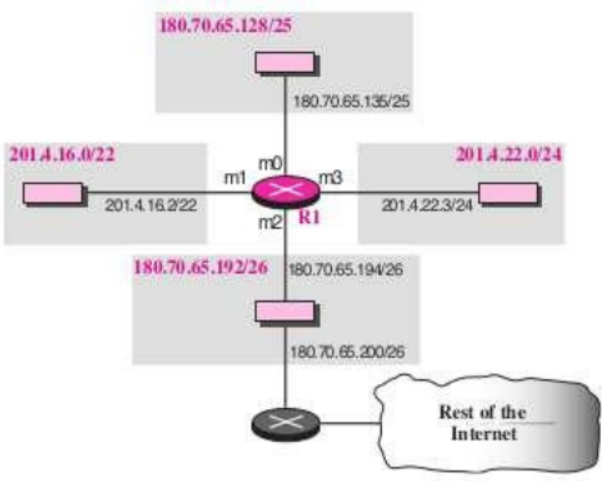
\includegraphics[width=0.8\textwidth]{assets/cap5/5.3.png}
\caption{Topologia de red del ejemplo con routers}
\label{fig:topologia-ejemplo}
\end{figure}

\subsection{Escalabilidad}

El encaminamiento con clase no es viable por el gran numero de redes. Soluciones:
\begin{itemize}
    \item \textbf{CIDR}: agregacion de direcciones y resumen de rutas.
    \item \textbf{Encaminamiento jerarquico}: limita la informacion intercambiada entre dominios.
\end{itemize}

\begin{figure}[H]
\centering
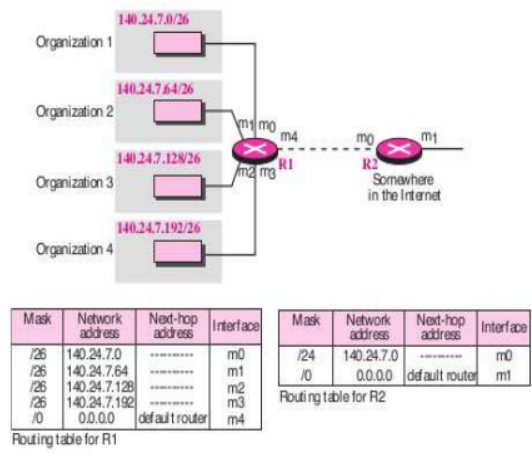
\includegraphics[width=0.8\textwidth]{assets/cap5/5.4.png}
\caption{Agregacion CIDR y jerarquia de encaminamiento}
\label{fig:cidr-jerarquia}
\end{figure}


\section{Tecnicas de Encaminamiento}

\subsection{Encaminamiento local}

No usa topologia global, solo informacion local.

\begin{itemize}
    \item \textbf{Aleatorio}: elige una salida al azar. Simple pero no optimo.
    \item \textbf{Aislado}: usa informacion local (mayor ancho de banda, menor congestion, round-robin).
    \item \textbf{Por inundacion (flooding)}: envia el paquete a todos los vecinos menos al origen.
\end{itemize}

\begin{definicion}
El \textbf{encaminamiento por inundacion (flooding)} es una tecnica en la que cada nodo reenvia el paquete recibido a todos sus vecinos excepto a aquel del que lo recibio. El destinatario puede recibir copias duplicadas, por lo que se usa un identificador unico para descartarlas. Se emplea el campo TTL para evitar bucles infinitos.
\end{definicion}

Ventajas del flooding: robusto, garantiza el camino mas corto, visita todos los nodos. Desventajas: saturacion por duplicados.

\begin{figure}[H]
\centering
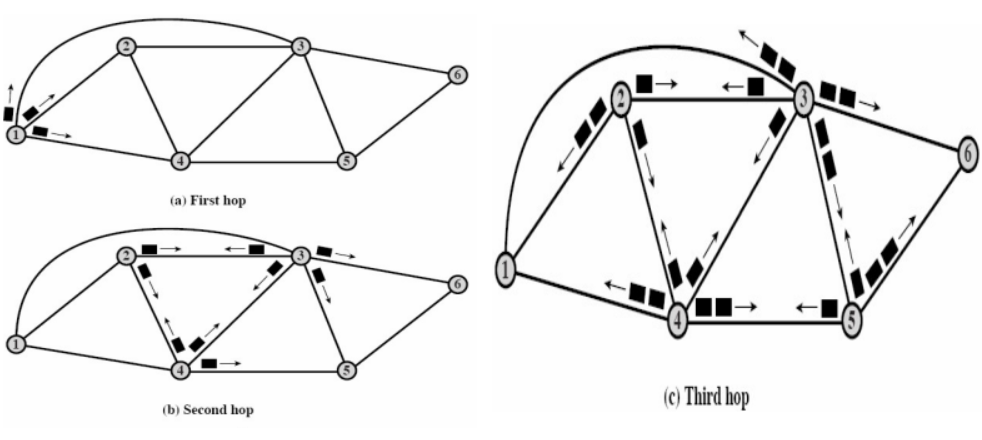
\includegraphics[width=0.8\textwidth]{assets/cap5/5.5.png}
\caption{Ejemplo de inundacion en red con multiples routers}
\label{fig:flooding-ejemplo}
\end{figure}

\subsection{Encaminamiento estatico}

Considera la topologia de la red. Las tablas se construyen \textbf{manualmente} y no se adaptan a cambios en la red.




\section{Vectores de Distancia}

\subsection{Fundamentos}

\begin{definicion}
En el \textbf{encaminamiento por vectores de distancia}, cada encaminador mantiene una entrada por cada destino posible con: destino, siguiente nodo y distancia/metria. El intercambio periodico de estos vectores con los vecinos permite que la red converja a caminos optimos mediante el algoritmo de \textbf{Bellman-Ford}. La metrica tipica es el \textbf{numero de saltos} (hop count).
\end{definicion}

\begin{figure}[H]
\centering
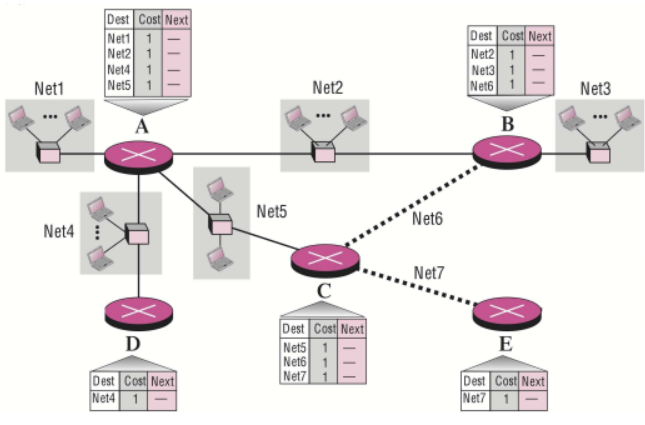
\includegraphics[width=0.8\textwidth]{assets/cap5/5.6.png}
\caption{Tabla de vectores de distancia inicial}
\label{fig:vectores-inicial}
\end{figure}

\subsection{Ejemplo de intercambio}

Inicialmente solo se conocen rutas directas. Tras el intercambio, cada router conoce la mejor ruta a todos los destinos.

\begin{figure}[H]
\centering
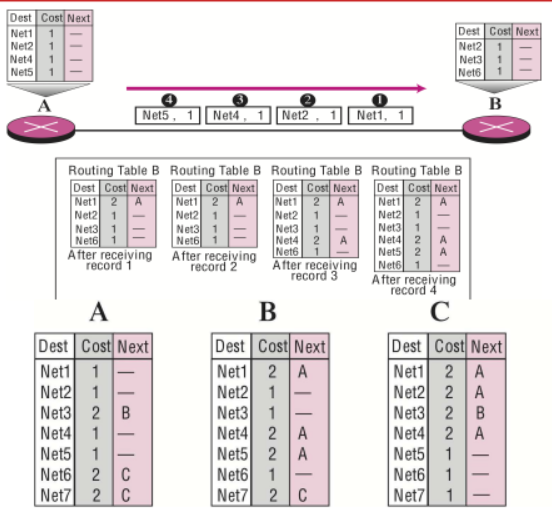
\includegraphics[width=0.8\textwidth]{assets/cap5/5.7.png}
\caption{Intercambio de vectores de distancia}
\label{fig:intercambio-vectores}
\end{figure}

\subsection{Problema: Cuenta a infinito}

Cuando un enlace cae o aumenta su coste, los cambios tardan en propagarse. Puede no converger debido a actualizaciones circulares que incrementan la metrica.

\begin{definicion}
La \textbf{cuenta a infinito (count-to-infinity)} es un problema de los protocolos por vectores de distancia en el que, tras un cambio negativo en la topologia, los routers incrementan ciclicamente sus metricas hasta alcanzar el limite establecido, provocando una convergencia muy lenta.
\end{definicion}

\subsection{Soluciones a la cuenta a infinito}

\begin{enumerate}
    \item \textbf{Limitar el infinito}: en RIP, 16 saltos = inalcanzable.
    \item \textbf{Horizonte dividido (split horizon)}: no se anuncia una ruta por la interfaz por la que se aprendio.
    \item \textbf{Horizonte dividido con respuesta envenenada (poisoned reverse)}: se anuncia con distancia infinita.
    \item \textbf{Actualizaciones forzadas (triggered updates)}: ante un cambio, se difunde inmediatamente.
\end{enumerate}

\begin{figure}[H]
\centering
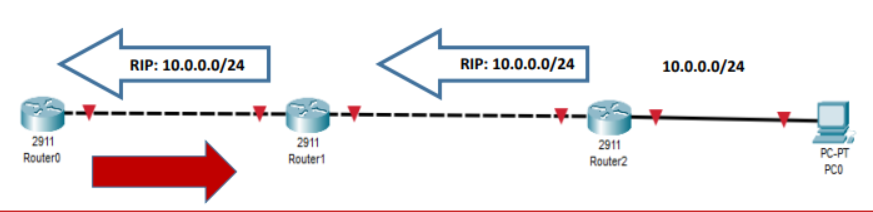
\includegraphics[width=0.8\textwidth]{assets/cap5/5.8.png}
\caption{Split horizon}
\label{fig:split-horizon}
\end{figure}

\begin{figure}[H]
\centering
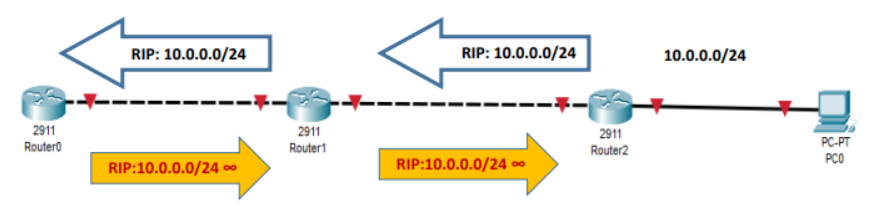
\includegraphics[width=0.8\textwidth]{assets/cap5/5.9.png}
\caption{Split horizon con poisoned reverse}
\label{fig:poisoned-reverse}
\end{figure}


\section{Encaminamiento en Internet}

\subsection{Sistemas Autonomos (AS)}

\begin{definicion}
Un \textbf{Sistema Autonomo (AS)} es un conjunto de redes y routers gestionados por una misma autoridad. Los \textbf{routers internos} usan protocolos IGP y solo conocen la organizacion de su AS. Los \textbf{routers frontera} (border routers) usan protocolos EGP y conocen el camino a otros AS, pero no su organizacion interna.
\end{definicion}

\begin{figure}[H]
\centering
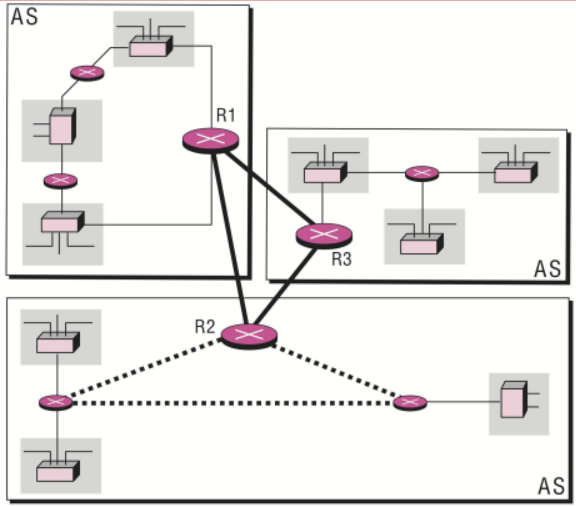
\includegraphics[width=0.8\textwidth]{assets/cap5/5.10.png}
\caption{Estructura de Internet con sistemas autonomos}
\label{fig:sistemas-autonomos}
\end{figure}

\subsection{Protocolos IGP (interior)}

\begin{itemize}
    \item \textbf{RIP} -- Routing Information Protocol
    \item \textbf{OSPF} -- Open Shortest Path First
    \item \textbf{IGRP} -- Internal Gateway Routing Protocol (Cisco)
\end{itemize}

\subsection{Protocolos EGP (exterior)}

\begin{itemize}
    \item \textbf{EGP} -- External Gateway Protocol
    \item \textbf{BGP} -- Border Gateway Protocol
\end{itemize}


\section{Practica 5: Encaminamiento en Internet con RIP}
\label{sec:practica5}

\subsection{Objetivos}

El objetivo de esta practica es profundizar en el concepto de encaminamiento en
redes de computadores, configurando routers con el protocolo de encaminamiento
\textbf{RIP} (Routing Information Protocol) en el simulador Cisco Packet Tracer.

\begin{enumerate}
    \item Comprender la diferencia entre encaminamiento estatico y dinamico.
    \item Configurar el protocolo RIP version 2 en multiples routers.
    \item Verificar que los routers intercambian informacion de rutas y convergen
    a la topologia de red.
    \item Comprobar la conectividad entre diferentes redes mediante traceroute y ping.
\end{enumerate}

\subsection{Material utilizado}

\begin{itemize}
    \item \textbf{Software}: Cisco Packet Tracer.
    \item \textbf{Hardware simulado}: 4 routers interconectados mediante enlaces seriales.
    \item \textbf{Redes involucradas}:
    \begin{itemize}
        \item 192.168.10.0/24 (LAN conectada a Router 0)
        \item 192.168.20.0/24 (LAN conectada a Router 3)
        \item 10.10.10.0/24 (enlace entre Router 0 y Router 2)
        \item 10.10.20.0/24 (enlace entre Router 1 y Router 2)
        \item 10.10.30.0/24 (enlace entre Router 0 y Router 1)
        \item 10.10.40.0/24 (enlace entre Router 2 y Router 3)
    \end{itemize}
\end{itemize}

\subsection{Desarrollo de la practica}

\subsubsection{Topologia de la red}

Se diseno una red con 4 routers interconectados mediante enlaces seriales,
formando una topologia mallada. Cada router tiene al menos una LAN conectada:

\begin{itemize}
    \item \textbf{Router 0}: conectado a la LAN 192.168.10.0/24 y a los enlaces
    10.10.10.0/24 (hacia Router 2) y 10.10.30.0/24 (hacia Router 1).
    \item \textbf{Router 1}: conectado al enlace 10.10.20.0/24 (hacia Router 2) y
    10.10.30.0/24 (hacia Router 0).
    \item \textbf{Router 2}: conectado a los enlaces 10.10.10.0/24 (hacia Router 0),
    10.10.20.0/24 (hacia Router 1) y 10.10.40.0/24 (hacia Router 3).
    \item \textbf{Router 3}: conectado a la LAN 192.168.20.0/24 y al enlace
    10.10.40.0/24 (hacia Router 2).
\end{itemize}

\begin{figure}[H]
\centering
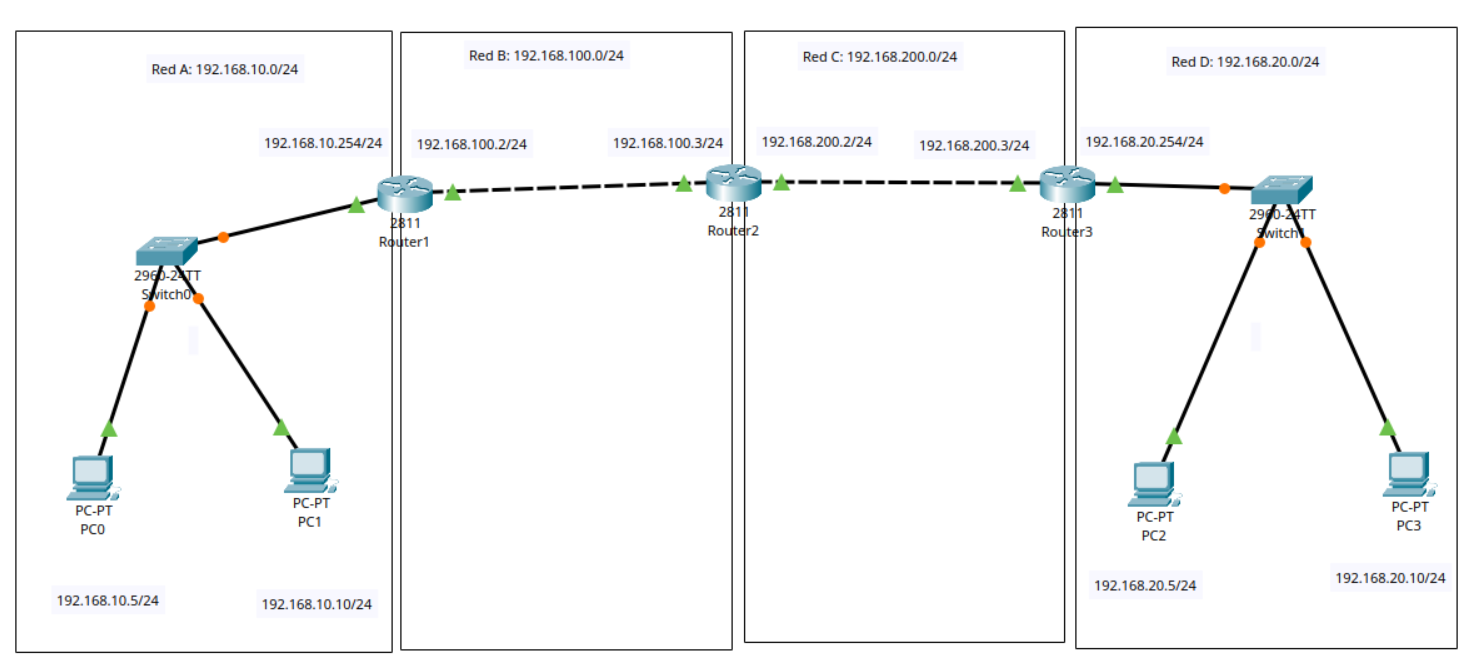
\includegraphics[width=0.8\textwidth]{assets/cap5/5.11.png}
\caption{Topologia de la red con 4 routers y encaminamiento RIP}
\label{fig:topologia-rip}
\end{figure}

\subsubsection{Configuracion de RIP en los routers}



\subsection{Relacion teoria-practica}

\begin{table}[htbp]
\centering
\small
\caption{Conexion entre conceptos teoricos y elementos de la Practica 5}
\begin{tabularx}{\textwidth}{@{}lX@{}}
\toprule
\textbf{Concepto teorico} & \textbf{Observacion/aplicacion en la practica} \\
\midrule
Encaminamiento estatico & Configuracion manual previa de rutas (alternativa mostrada en el enunciado) \\
Encaminamiento dinamico & RIP permite que los routers aprendan rutas automaticamente sin intervencion manual \\
Protocolo RIP (vector distancia) & Cada router intercambia periodicamente su tabla con los vecinos, usando saltos como metrica \\
Convergencia & Tras configurar RIP, los routers necesitan un tiempo para intercambiar tablas y alcanzar rutas estables \\
Tabla de encaminamiento & \texttt{show ip route} muestra rutas directamente conectadas (C) y aprendidas por RIP (R) \\
Distancia administrativa & 120 es la distancia administrativa de RIP; menor valor implica mayor confianza \\
Metrica de saltos & \texttt{[120/2]} indica 2 saltos hasta la red remota; RIP maximo 15 saltos \\
Next-hop & \texttt{via 10.10.10.2} indica la direccion IP del siguiente router al que reenviar el paquete \\
TTL (Time To Live) & El TTL decrece en cada salto; un valor de 253 indica 3 routers atravesados \\
Passive-interface & Evita enviar actualizaciones RIP por la interfaz LAN, reduciendo trafico innecesario \\
\bottomrule
\end{tabularx}
\end{table}


\section{Resumen de la Unidad 5}

\begin{itemize}
    \item El \textbf{encaminamiento} es la eleccion del camino optimo para un paquete; la \textbf{conmutacion} es el reenvio por ese camino.
    \item Los \textbf{grafos} modelan las redes: nodos son routers, enlaces son conexiones. Se representan mediante listas o matrices de adyacencia.
    \item Los \textbf{algoritmos de camino mas corto} como Dijkstra y Bellman-Ford permiten calcular rutas optimas. El \textbf{Minimum Spanning Tree} es util para difusion y evitacion de bucles.
    \item Las \textbf{tablas de encaminamiento} almacenan destino, mascara, siguiente salto y coste. El principio \textbf{next-hop} permite que cada router solo conozca el siguiente paso.
    \item Las \textbf{tecnicas de encaminamiento} incluyen: local (aleatorio, aislado, flooding), estatico (manual) y dinamico (vectores de distancia o estado de enlace).
    \item El \textbf{encaminamiento por vectores de distancia} usa Bellman-Ford e intercambio periodico de tablas. Sufre el problema de \textbf{cuenta a infinito}, resuelto con horizonte dividido, poisoned reverse y triggered updates.
    \item Los \textbf{protocolos de encaminamiento} se clasifican en: vector de distancia (RIP, Bellman-Ford) y estado de enlace (OSPF, Dijkstra).
    \item El \textbf{encaminamiento jerarquico} organiza Internet en Sistemas Autonomos (AS), usando protocolos IGP (RIP, OSPF) internamente y EGP (BGP) entre AS.
    \item \textbf{RIP} es un protocolo IGP por vectores de distancia con metrica de saltos, limite de 16, temporizadores periodicos (30s), de expiracion (180s) y de basura (120s).
    \item La \textbf{Practica 5} demuestra la configuracion de RIPv2 en una red de 4 routers, la convergencia de tablas, la verificacion con \texttt{show ip route}, \texttt{ping} y \texttt{traceroute}.
\end{itemize}

%%%%%%%%%%%%%%%%%%%%%%%%%%%%%%%%%%%%%%%%%%%%%%%%%%%%%%%%%%%%%%%%%%%%%%%%%%%%%%%
%                         CAPITULO 6
%           Protocolos de Comunicacion y Redes CAN
%%%%%%%%%%%%%%%%%%%%%%%%%%%%%%%%%%%%%%%%%%%%%%%%%%%%%%%%%%%%%%%%%%%%%%%%%%%%%%%

\chapter{Protocolos de Comunicacion y Redes CAN}

Hasta ahora hemos visto como se comunican dispositivos mediante UART, RS-232,
Wi-Fi, Bluetooth y redes TCP/IP. En el entorno industrial, sin embargo, existen
protocolos especificos diseñados para conectar sensores, actuadores, PLCs y
sistemas de control en tiempo real. Estos protocolos deben ser robustos, rapidos
y capaces de operar en entornos con ruido electrico y grandes distancias.

En este capitulo estudiamos los protocolos de comunicacion mas relevantes en
la industria: I2C, SPI, RS-485, Modbus y CAN. Cada uno tiene sus ventajas y
se emplea segun las necesidades de velocidad, distancia, numero de nodos y
fiabilidad del sistema.


%=============================================================================
\section{I2C: Inter-Integrated Circuit}
%=============================================================================

\subsection{Que es I2C}

El bus I2C (abreviatura de \textit{Inter-Integrated Circuits}) es un protocolo de
comunicacion serie sincrona desarrollado por Philips en 1982. Se diseño para
conectar circuitos integrados de baja velocidad dentro de un mismo dispositivo
o placa, como microcontroladores, sensores, memorias EEPROM y pantallas.

\begin{definicion}[I2C]
El \textbf{bus I2C} es un protocolo de comunicacion serie sincrono que utiliza
dos lineas para transmitir datos entre dispositivos: una linea de reloj (SCL) y
una linea de datos (SDA). Permite la conexion de multiples dispositivos en una
arquitectura de bus con multiples maestros y multiples esclavos.
\end{definicion}

La principal ventaja del I2C es su sencillez: solo necesita dos lineas de senal
mas masa (GND), lo que reduce el numero de pines necesarios en los
microcontroladores. Ademas, al ser un bus multi-maestro, cualquier dispositivo
conectado puede iniciar una transferencia si el bus esta libre.

\subsection{Senalizacion}

El bus I2C utiliza tres conexiones basicas:

\begin{itemize}
    \item \textbf{SCL} (\textit{System Clock}): linea de reloj que sincroniza la
    comunicacion entre todos los dispositivos. El maestro genera los pulsos de
    reloj.
    \item \textbf{SDA} (\textit{System Data}): linea de datos por la que se
    transfieren los bits de informacion entre maestro y esclavo.
    \item \textbf{GND} (Masa): referencia de tension comun para todos los
    dispositivos conectados al bus.
\end{itemize}

Ambas lineas (SCL y SDA) son \textit{open-drain} o \textit{open-collector}, lo que
significa que cada dispositivo solo puede poner la linea a nivel bajo (0) o
liberarla (1). Por eso se necesitan resistencias de pull-up externas
conectadas a la alimentacion (tipicamente 4.7 k$\Omega$ a 3.3 V o 5 V).

% TODO: imagen
\begin{figure}[H]
    \centering
    \fbox{\parbox{0.8\textwidth}{
        \centering
        \vspace{1cm}
        TODO: Esquema del bus I2C con maestro, dos esclavos y resistencias de pull-up.
        \vspace{1cm}
    }}
    \caption{Esquema basico del bus I2C con resistencias de pull-up.}
    \label{fig:i2c_esquema}
\end{figure}

\subsection{Transferencia de datos}

La comunicacion en I2C siempre la inicia un \textbf{maestro}. Cada esclavo tiene
una direccion unica de 7 bits (o 10 bits en modo extendido), que el maestro
envia al principio de cada transaccion.

\textbf{Escritura en un dispositivo esclavo:}

\begin{enumerate}
    \item El maestro envia una \textbf{condicion de inicio} (START): SDA pasa de
    alto a bajo mientras SCL permanece en alto.
    \item Envio de la \textbf{direccion del esclavo} (7 bits) mas el bit de
    lectura/escritura (0 = escritura).
    \item El esclavo responde con un bit de \textbf{reconocimiento} (ACK).
    \item El maestro envia la \textbf{direccion del registro interno} donde quiere
    escribir.
    \item El esclavo responde con ACK.
    \item El maestro envia el \textbf{byte de dato}.
    \item El esclavo responde con ACK.
    \item [Opcionalmente] se pueden enviar mas bytes de datos.
    \item El maestro envia una \textbf{condicion de parada} (STOP): SDA pasa de
    bajo a alto mientras SCL esta en alto.
\end{enumerate}

\textbf{Lectura desde un dispositivo esclavo:}

\begin{enumerate}
    \item Condicion de inicio (START).
    \item Direccion del esclavo con bit de escritura (0).
    \item ACK del esclavo.
    \item Envio de la direccion del registro interno a leer.
    \item ACK del esclavo.
    \item \textbf{Condicion de inicio reiterada} (Repeated START).
    \item Direccion del esclavo con bit de lectura (1).
    \item ACK del esclavo.
    \item El esclavo envia el \textbf{byte de dato}.
    \item El maestro responde con ACK (si quiere leer mas) o NACK (fin de lectura).
    \item Condicion de parada (STOP).
\end{enumerate}

\subsection{Ejemplo practico: sensor brujula digital CMPS03}

El sensor CMPS03 es una brujula digital que mide el campo magnetico terrestre
para determinar la orientacion. Una vez calibrado, ofrece una precision de 3 a 4
grados con resolucion de decimas.

Este sensor dispone de dos interfaces de salida:
\begin{itemize}
    \item \textbf{PWM} (modulacion en anchura de pulso): un pin genera pulsos cuya
    duracion es proporcional al angulo.
    \item \textbf{I2C}: permite leer el angulo directamente como un byte (0--255)
    o como dos bytes (0--3599, resolucion de 0.1 grados).
\end{itemize}

Para leer el angulo por I2C, el procedimiento es:
\begin{enumerate}
    \item Enviar START y la direccion del CMPS03 (0xC0) con bit de escritura.
    \item Enviar la direccion del registro interno 0x01 (angulo en 0--255).
    \item Enviar Repeated START.
    \item Enviar la direccion del CMPS03 (0xC1) con bit de lectura.
    \item Leer el byte de dato que contiene el angulo.
    \item Enviar STOP.
\end{enumerate}


%=============================================================================
\section{SPI: Serial Peripheral Interface}
%=============================================================================

\subsection{Que es SPI}

SPI es un protocolo de comunicacion serie sincrona desarrollado por Motorola en
1982. A diferencia de I2C, SPI esta pensado para alcanzar velocidades muy
superiores y opera en modo \textbf{full-duplex}, lo que significa que puede enviar
y recibir datos simultaneamente.

\begin{definicion}[SPI]
El \textbf{bus SPI} (\textit{Serial Peripheral Interface}) es un protocolo de
comunicacion serie sincrona de cuatro hilos que permite la transmision full-duplex
entre un dispositivo maestro y uno o varios esclavos. Utiliza lineas separadas
para reloj (SCK), datos de salida (MOSI), datos de entrada (MISO) y seleccion de
esclavo (SS).
\end{definicion}

SPI se utiliza habitualmente para comunicar un microcontrolador con perifericos
de alta velocidad como memorias Flash, pantallas TFT, convertidores ADC/DAC y
modulos de comunicacion.

\subsection{Senales del bus SPI}

Un bus SPI completo utiliza cuatro lineas:

\begin{itemize}
    \item \textbf{SCK} (\textit{Serial Clock}): senal de reloj generada por el
    maestro. Sincroniza la transmision de datos.
    \item \textbf{MOSI} (\textit{Master Out Slave In}): linea de datos del
    maestro al esclavo. El maestro envia informacion por esta linea.
    \item \textbf{MISO} (\textit{Master In Slave Out}): linea de datos del
    esclavo al maestro. El esclavo responde por esta linea.
    \item \textbf{SS} o \textbf{CS} (\textit{Slave Select} / \textit{Chip
    Select}): linea de control que el maestro utiliza para seleccionar a que
    esclavo se dirige. Normalmente activa en nivel bajo.
\end{itemize}

% TODO: imagen
\begin{figure}[H]
    \centering
    \fbox{\parbox{0.8\textwidth}{
        \centering
        \vspace{1cm}
        TODO: Esquema SPI con maestro, dos esclavos y lineas SCK, MOSI, MISO, SS.
        \vspace{1cm}
    }}
    \caption{Esquema del bus SPI con un maestro y dos esclavos.}
    \label{fig:spi_esquema}
\end{figure}

\subsection{Funcionamiento}

En SPI, el maestro siempre genera el reloj (SCK). En cada pulso de reloj, se
transfiere un bit en ambas direcciones simultaneamente: un bit sale por MOSI
y otro entra por MISO. Esto permite el modo full-duplex.

El maestro debe conocer de antemano cuantos bits espera recibir del esclavo,
porque debe mantener el reloj activo durante toda la transferencia. Si el esclavo
necesita tiempo para preparar la respuesta, el maestro puede introducir
pequenas pausas entre bytes.

\textbf{Seleccion de esclavo:}

Existen dos formas de conectar multiples esclavos:

\begin{enumerate}
    \item \textbf{SS independiente}: cada esclavo tiene su propia linea SS
    conectada al maestro. El maestro activa (baja) solo la linea del esclavo
    con el que quiere comunicarse.
    \item \textbf{Conexion en cascada (daisy chain)}: los esclavos se conectan
    en serie. El maestro envia datos a traves de todos los esclavos
    consecutivamente, como una cadena de registros de desplazamiento.
\end{enumerate}

\subsection{Comparacion: SPI vs I2C vs UART}

\begin{table}[H]
    \centering
    \caption{Comparativa de protocolos de comunicacion serie}
    \label{tab:comparativa_spi_i2c_uart}
    \small
    \begin{tabular}{|l|c|c|c|}
        \hline
        \textbf{Caracteristica} & \textbf{SPI} & \textbf{I2C} & \textbf{UART} \\
        \hline
        Tipo de senal & Sincrona & Sincrona & Asincrona \\
        \hline
        Modo duplex & Full-duplex & Half-duplex & Full-duplex \\
        \hline
        Numero de lineas & 4 (o mas) & 2 & 2 (TX/RX) \\
        \hline
        Velocidad tipica & Hasta 10+ Mbps & Hasta 3.4 Mbps & Hasta 1 Mbps \\
        \hline
        Maestros & Uno (tipico) & Multiples & Ninguno (peer-to-peer) \\
        \hline
        Esclavos & Multiples (por SS) & Multiples (por direccion) & 1 \\
        \hline
        Direccionamiento & Por linea SS & Por direccion 7/10 bits & Ninguno \\
        \hline
        Distancia & Corta (placa) & Corta (placa) & Media (15 m RS-232) \\
        \hline
    \end{tabular}
\end{table}

\textbf{Ventajas de SPI:}
\begin{itemize}
    \item Mayor velocidad que I2C y UART.
    \item Full-duplex: envia y recibe simultaneamente.
    \item El tamano de los mensajes puede ser arbitrario.
    \item Hardware sencillo y de bajo coste.
    \item Los esclavos no necesitan oscilador propio (el reloj lo genera el maestro).
\end{itemize}

\textbf{Desventajas de SPI:}
\begin{itemize}
    \item Necesita mas pines que I2C (especialmente si hay muchos esclavos).
    \item No hay confirmacion de recepcion por parte del esclavo (no hay ACK).
    \item Solo admite un maestro en la mayoria de implementaciones.
    \item Distancias muy cortas (dentro de la misma placa).
    \item El maestro debe conocer de antemano la longitud de la respuesta.
\end{itemize}


%=============================================================================
\section{RS-485: Comunicacion diferencial robusta}
%=============================================================================

\subsection{Introduccion}

RS-485 es un estandar de comunicacion serie muy utilizado en aplicaciones de
adquisicion de datos y control industrial. Su principal ventaja es la capacidad
de conectar multiples dispositivos en el mismo bus (hasta 32 transmisores y 32
receptores tipicamente) sobre distancias de hasta 1200 metros.

\begin{definicion}[RS-485]
El estandar \textbf{RS-485} (tambien conocido como EIA-485) define una interfaz
de comunicacion serie multipunto con transmision diferencial balanceada. Permite
la conexion de multiples transmisores y receptores en un bus semiduplex, siendo
altamente resistente al ruido electrico y apto para largas distancias.
\end{definicion}

\subsection{Caracteristicas principales}

Las caracteristicas mas destacadas de RS-485 son:

\begin{itemize}
    \item \textbf{Transmision diferencial}: los datos se envian mediante un par
    trenzado de hilos (A y B). Un hilo transmite la senal original y el otro su
    copia invertida. El receptor detecta la \textbf{diferencia de voltaje} entre
    ambos, lo que elimina el ruido comun que afecta por igual a ambos hilos.
    \item \textbf{Multipunto}: permite conectar hasta 32 dispositivos (transmisores
    y receptores) en el mismo bus. Con repetidores o transceivers avanzados se
    puede extender a mas nodos.
    \item \textbf{Semiduplex}: los dispositivos pueden enviar y recibir, pero no
    simultaneamente. En un instante dado, solo un equipo puede transmitir,
    mientras que todos los demas pueden recibir.
    \item \textbf{Inmunidad al ruido}: la transmision diferencial y el uso de par
    trenzado (a veces blindado) garantizan una alta resistencia a
    interferencias electromagneticas.
\end{itemize}

\subsection{Niveles de senal y cableado}

En RS-485, el estado logico se determina por la diferencia de voltaje entre las
lineas A y B:

\begin{itemize}
    \item \textbf{Bit 1 (Marca / recessive)}: $V_A - V_B < -200$ mV.
    \item \textbf{Bit 0 (Espacio / dominant)}: $V_A - V_B > +200$ mV.
\end{itemize}

El cableado basico consiste en un par trenzado para los datos (A y B), mas
lineas opcionales de alimentacion (0 V y 5 V) para alimentar dispositivos del
bus. Es recomendable colocar \textbf{terminaciones de linea} (resistencias de 120
$\Omega$) al principio y al final del bus para evitar reflexiones de senal.

% TODO: imagen
\begin{figure}[H]
    \centering
    \fbox{\parbox{0.8\textwidth}{
        \centering
        \vspace{1cm}
        TODO: Esquema de bus RS-485 con par trenzado, terminaciones de 120 Ohm
        y varios nodos conectados.
        \vspace{1cm}
    }}
    \caption{Topologia tipica de un bus RS-485 con terminaciones.}
    \label{fig:rs485_topologia}
\end{figure}

\subsection{Distancia vs velocidad}

Una regla practica en RS-485 es que el producto de la longitud del cable (en
metros) por la velocidad de datos (en bits por segundo) no debe superar
$10^8$:

\begin{equation}
    \mathrm{Longitud\,(m)} \times \mathrm{Velocidad\,(bps)} \leq 10^8
\end{equation}

\begin{table}[H]
    \centering
    \caption{Relacion entre distancia y velocidad en RS-485}
    \label{tab:rs485_distancia}
    \begin{tabular}{|c|c|}
        \hline
        \textbf{Distancia} & \textbf{Velocidad maxima aproximada} \\
        \hline
        15 m & 10 Mbps \\
        \hline
        100 m & 1 Mbps \\
        \hline
        500 m & 200 kbps \\
        \hline
        1200 m & 100 kbps \\
        \hline
    \end{tabular}
\end{table}

\subsection{RS-232 vs RS-485}

\begin{table}[H]
    \centering
    \caption{Comparativa entre RS-232 y RS-485}
    \label{tab:rs232_vs_rs485}
    \begin{tabular}{|l|c|c|}
        \hline
        \textbf{Caracteristica} & \textbf{RS-232} & \textbf{RS-485} \\
        \hline
        Tipo de comunicacion & Punto a punto & Multipunto \\
        \hline
        Duplex & Full-duplex & Semiduplex \\
        \hline
        Tipo de senal & Desbalanceada (unipolar) & Balanceada (diferencial) \\
        \hline
        Niveles de voltaje & $\pm 3$ V a $\pm 15$ V & Diferencial 200 mV \\
        \hline
        Max. dispositivos & 1 TX + 1 RX & 32 TX + 32 RX (estandar) \\
        \hline
        Velocidad maxima & 1 Mbps a 15 m & 10 Mbps a 15 m \\
        \hline
        Distancia maxima & $\sim$ 15 m & $\sim$ 1200 m a 100 kbps \\
        \hline
        Inmunidad al ruido & Baja & Alta \\
        \hline
        Lineas de control & DTR, DSR, RTS, CTS & Ninguna (solo datos) \\
        \hline
    \end{tabular}
\end{table}


%=============================================================================
\section{Modbus: protocolo de comunicacion industrial}
%=============================================================================

\subsection{Que es Modbus}

Modbus es uno de los protocolos de comunicacion mas extendidos en la
automatizacion industrial. Fue desarrollado en 1979 por Modicon (hoy Schneider
Electric) para su gama de PLCs. Hoy en dia es un estandar abierto que permite
la comunicacion entre controladores, sensores, actuadores y sistemas SCADA.

\begin{definicion}[Modbus]
El protocolo \textbf{Modbus} es un protocolo de comunicacion abierto para la
transmision de datos entre dispositivos electronicos en entornos industriales.
Se situa en los niveles 1, 2 y 7 del modelo OSI. Funciona sobre arquitectura
maestro/esclavo (en RTU) o cliente/servidor (en TCP/IP).
\end{definicion}

Modbus es independiente del medio fisico: puede funcionar sobre RS-232,
RS-485, Ethernet TCP/IP, o incluso por radio. Esto lo hace extremadamente
versatil.

\subsection{Variantes de Modbus}

A lo largo de los años han aparecido diferentes variantes de Modbus adaptadas a
diversos medios fisicos:

\begin{table}[H]
    \centering
    \caption{Variantes del protocolo Modbus}
    \label{tab:modbus_variantes}
    \begin{tabular}{|l|p{8cm}|}
        \hline
        \textbf{Variante} & \textbf{Descripcion} \\
        \hline
        Modbus RTU & Implementacion mas comun. Usa comunicacion serie (RS-232/RS-485)
        con representacion binaria compacta de los datos. Requiere CRC para
        verificacion. \\
        \hline
        Modbus ASCII & Usa comunicacion serie con caracteres ASCII. Mas lento que
        RTU. Utiliza checksum LRC. \\
        \hline
        Modbus TCP/IP & Funciona sobre Ethernet TCP/IP, puerto 502. No requiere
        checksum adicional porque TCP ya lo proporciona. \\
        \hline
        Modbus RTU sobre IP & Similar a Modbus TCP pero incluye CRC en la carga
        util, como en RTU. \\
        \hline
        Modbus UDP & Variante experimental sobre UDP para reducir overhead. \\
        \hline
        Modbus Plus (MB+) & Version propietaria de Schneider Electric. Soporta
        comunicacion peer-to-peer entre multiples maestros. Requiere hardware
        especial (co-procesador HDLC). \\
        \hline
    \end{tabular}
\end{table}

\subsection{Modbus RTU en detalle}

Modbus RTU (\textit{Remote Terminal Unit}) es la variante mas utilizada en el
entorno industrial. Se basa en una arquitectura \textbf{maestro-esclavo} sobre
un bus serie (generalmente RS-485).

\textbf{Estructura de la trama RTU:}

\begin{table}[H]
    \centering
    \caption{Formato de trama Modbus RTU}
    \label{tab:modbus_trama}
    \begin{tabular}{|l|c|p{6cm}|}
        \hline
        \textbf{Campo} & \textbf{Tamano} & \textbf{Descripcion} \\
        \hline
        Direccion del esclavo & 1 byte & Identifica el dispositivo destino (1--247) \\
        \hline
        Codigo de funcion & 1 byte & Indica la operacion a realizar (leer, escribir, etc.) \\
        \hline
        Datos & N bytes & Parametros de la funcion y valores \\
        \hline
        CRC & 2 bytes & Codigo de redundancia ciclica para deteccion de errores \\
        \hline
    \end{tabular}
\end{table}

El dispositivo \textbf{maestro} (por ejemplo un PLC o sistema SCADA) inicia la
comunicacion enviando una trama al esclavo. Solo el esclavo con la direccion
indicada responde. Los demas escuchan pero ignoran el mensaje.

\textbf{Codigos de funcion mas comunes:}
\begin{itemize}
    \item \textbf{01}: Leer bobinas (coils) -- salidas digitales.
    \item \textbf{02}: Leer entradas digitales.
    \item \textbf{03}: Leer registros de retencion (holding registers) -- 16 bits.
    \item \textbf{04}: Leer registros de entrada (input registers).
    \item \textbf{05}: Escribir una bobina.
    \item \textbf{06}: Escribir un registro de retencion.
    \item \textbf{15}: Escribir multiples bobinas.
    \item \textbf{16}: Escribir multiples registros.
\end{itemize}

\subsection{RS-232 vs RS-485 en Modbus}

La eleccion entre RS-232 y RS-485 depende de las necesidades de la aplicacion:

\begin{itemize}
    \item \textbf{RS-232}: adecuado para conexiones punto a punto a corta distancia
    (hasta 15 m). Usa conectores DB9 o DB25. Ideal para conectar un PLC
    directamente a un panel HMI o a un PC de programacion.
    \item \textbf{RS-485}: emplea un esquema de bus multidrop que permite conectar
    multiples dispositivos en la misma linea. Ideal para distancias largas
    (hasta 1200 m) y entornos con ruido electrico. Es el estandar de facto en
    redes de campo industriales.
\end{itemize}


%=============================================================================
\section{CAN: Controller Area Network}
%=============================================================================

\subsection{Introduccion}

CAN (\textit{Controller Area Network}) es un bus de comunicaciones serie
diseñado originalmente por Bosch en 1986 para la industria automotriz. Hoy en
dia es un estandar internacional (ISO 11898) y se emplea ampliamente en
automocion, maquinaria industrial, robots, sistemas medicos y avionica.

\begin{definicion}[CAN]
El \textbf{bus CAN} (\textit{Controller Area Network}) es un protocolo de
comunicacion de datos en serie de alta integridad para aplicaciones en tiempo
real. Utiliza un bus de dos hilos con arbitraje basado en prioridad, difusion de
mensajes, y excelentes capacidades de deteccion de errores y confinamiento de
fallos.
\end{definicion}

CAN se distingue de otros protocolos porque no utiliza direcciones de nodo.
En su lugar, cada mensaje lleva un \textbf{identificador} que define tanto la
prioridad como el contenido del mensaje. Cualquier nodo puede enviar un
mensaje cuando el bus esta libre, y todos los demas nodos reciben ese mensaje,
decidiendo individualmente si les interesa o no.

\subsection{Caracteristicas principales}

Las caracteristicas mas destacadas de CAN son:

\begin{itemize}
    \item \textbf{Acceso multi-maestro}: cualquier nodo puede iniciar la
    transmision cuando el bus esta libre.
    \item \textbf{Difusion de mensajes} (broadcast): todos los nodos reciben cada
    mensaje. No hay comunicacion punto a punto.
    \item \textbf{Prioridad de mensajes}: el identificador determina la prioridad.
    Los mensajes con identificador mas bajo tienen mayor prioridad.
    \item \textbf{Longitud limitada}: hasta 8 bytes de datos por mensaje.
    \item \textbf{Velocidad}: hasta 1 Mbit/s en distancias cortas (hasta 40 m a 1
    Mbps; 125 kbps a 500 m aproximadamente).
    \item \textbf{Deteccion de errores}: mecanismos de supervision de bits,
    CRC, reconocimiento y relleno de bits garantizan una tasa de error
    residual extremadamente baja.
\end{itemize}

\subsection{Tipos de tramas CAN}

En CAN existen cuatro tipos de tramas:

\begin{enumerate}
    \item \textbf{Trama de datos}: transmite un mensaje al bus. Contiene el
    identificador, los datos (0--8 bytes) y campos de control y CRC.
    \item \textbf{Trama remota}: solicita la transmision de un mensaje con un
    identificador especifico. Un nodo que produzca ese mensaje respondera
    enviando la trama de datos correspondiente.
    \item \textbf{Trama de error}: cualquier nodo que detecte una condicion de
    error envia una trama de error para notificar a todos los demas nodos.
    \item \textbf{Trama de sobrecarga}: similar a la trama de error, pero indica
    que un nodo no esta listo para recibir mas datos y necesita un retraso.
\end{enumerate}

\subsection{Formato de trama de datos}

Una trama de datos CAN (formato estandar con identificador de 11 bits) contiene
los siguientes campos:

\begin{table}[H]
    \centering
    \caption{Campos de una trama de datos CAN (formato estandar)}
    \label{tab:can_trama}
    \begin{tabular}{|l|c|p{6cm}|}
        \hline
        \textbf{Campo} & \textbf{Bits} & \textbf{Descripcion} \\
        \hline
        Inicio de trama (SOF) & 1 & Bit dominante que marca el inicio \\
        \hline
        Identificador + RTR & 12 & 11 bits de ID + 1 bit RTR (Remote Transmission Request) \\
        \hline
        Control & 6 & Indica tamano de datos y formato (estandar/extendido) \\
        \hline
        Datos & 0--64 & De 0 a 8 bytes de informacion util \\
        \hline
        CRC & 15 + 1 & Codigo de redundancia ciclica + delimitador \\
        \hline
        ACK & 2 & Ventana de reconocimiento por parte de los receptores \\
        \hline
        Fin de trama (EOF) & 7 & Bits recesivos que marcan el final \\
        \hline
        Intermission (IFS) & 3 & Tiempo minimo entre tramas \\
        \hline
    \end{tabular}
\end{table}

\textbf{Formato estandar vs extendido:}

\begin{itemize}
    \item \textbf{CAN estandar} (CAN 2.0A): identificador de 11 bits (2048
    mensajes posibles, aunque algunos IDs estan reservados).
    \item \textbf{CAN extendido} (CAN 2.0B): identificador de 29 bits (mas de 500
    millones de mensajes posibles).
\end{itemize}

Ambos formatos pueden coexistir en el mismo bus. La distincion se realiza
mediante el bit \textbf{IDE} (Identifier Extension).

\subsection{Arbitraje de bus: dominante y recesivo}

CAN utiliza un mecanismo de arbitraje \textbf{no destructivo} basado en los
niveles logicos del bus:

\begin{itemize}
    \item \textbf{Nivel dominante} (0 logico): el estado que impone su valor
    cuando un nodo lo transmite.
    \item \textbf{Nivel recesivo} (1 logico): el estado que solo se mantiene si
    \textit{ningun} nodo transmite un dominante.
\end{itemize}

El bus CAN es como una \textbf{AND cableada}: si un nodo pone dominante y otro
recesivo, el resultado es dominante. Esto permite que varios nodos comiencen a
transmitir simultaneamente, pero solo el que envie el mensaje con el
\textbf{identificador mas bajo} (mas dominantes en los primeros bits) gane el
arbitraje.

\textbf{Proceso de arbitraje:}
\begin{enumerate}
    \item Dos o mas nodos detectan que el bus esta libre y comienzan a transmitir
    al mismo tiempo.
    \item Cada nodo envia su identificador bit a bit.
    \item Cada nodo transmisor supervisa el nivel real del bus.
    \item Si un nodo envia un recesivo (1) pero ve un dominante (0) en el bus,
    significa que otro nodo tiene un identificador con mayor prioridad (ID mas
    bajo). Este nodo se retira y pasa a modo receptor.
    \item El nodo con el ID mas bajo gana el arbitraje y continua transmitiendo
    sin perdida de tiempo ni datos.
    \item Los nodos que perdieron reintentaran automaticamente cuando el bus vuelva
    a estar libre.
\end{enumerate}

% TODO: imagen
\begin{figure}[H]
    \centering
    \fbox{\parbox{0.8\textwidth}{
        \centering
        \vspace{1cm}
        TODO: Diagrama temporal de arbitraje CAN con dos nodos compitiendo.
        Nodo A (ID 0x123) gana sobre Nodo B (ID 0x456).
        \vspace{1cm}
    }}
    \caption{Arbitraje no destructivo en el bus CAN.}
    \label{fig:can_arbitraje}
\end{figure}

\subsection{Supervision de bits y relleno de bits}

\textbf{Supervision de bits (bit monitoring):}
Cada nodo transmisor supervisa el nivel del bus bit a bit y lo compara con lo
que el mismo esta enviando. Si detecta una discrepancia, sabe que ha ocurrido
un error (o que perdio el arbitraje).

\textbf{Relleno de bits (bit stuffing):}
Para garantizar suficientes transiciones en el bus (necesarias para la
sincronizacion), CAN inserta un bit de polaridad opuesta despues de 5 bits
consecutivos del mismo valor. Este bit de relleno es transparente para la capa
superior y se elimina en recepcion.

La longitud de la trama varia debido al relleno. En el peor caso (identificador
de 11 bits, datos maximos):

\begin{table}[H]
    \centering
    \caption{Longitud de trama CAN con relleno de bits}
    \label{tab:can_longitud}
    \begin{tabular}{|c|c|c|c|}
        \hline
        \textbf{Datos} & \textbf{Sin relleno} & \textbf{Promedio} & \textbf{Peor caso} \\
        \hline
        0 bytes & 47 bits & 49 bits & 55 bits \\
        \hline
        8 bytes & 111 bits & 114 bits & 135 bits \\
        \hline
    \end{tabular}
\end{table}

\subsection{Errores y confinamiento de fallos}

CAN dispone de sofisticados mecanismos para detectar y gestionar errores:

\textbf{Tipos de errores:}
\begin{enumerate}
    \item \textbf{Error de bit}: un transmisor envia un bit pero lee el nivel
    opuesto en el bus.
    \item \textbf{Error de relleno}: se detectan 6 bits consecutivos del mismo
    valor.
    \item \textbf{Error CRC}: el calculo CRC del receptor no coincide con el
    campo CRC recibido.
    \item \textbf{Error de formato}: bits de formato fijo en posiciones incorrectas.
    \item \textbf{Error de reconocimiento (ACK)}: ningun receptor envio un ACK
    dominante.
\end{enumerate}

\textbf{Confinamiento de fallos (fault confinement):}
Cada nodo CAN mantiene dos contadores de errores:
\begin{itemize}
    \item \textbf{TEC} (\textit{Transmit Error Counter}): cuenta errores en
    transmision.
    \item \textbf{REC} (\textit{Receive Error Counter}): cuenta errores en
    recepcion.
\end{itemize}

Segun el valor de estos contadores, un nodo puede estar en tres estados:
\begin{enumerate}
    \item \textbf{Activo} (Error Active): estado normal. El nodo puede enviar
    tramas de error activas (6 bits dominantes).
    \item \textbf{Pasivo} (Error Passive): cuando un contador supera 127. El nodo
    solo puede enviar tramas de error pasivas (6 bits recesivos) y debe esperar
    8 bits adicionales antes de retransmitir.
    \item \textbf{Bus Off}: cuando TEC supera 255. El nodo se desconecta del bus
    y no puede transmitir ni recibir hasta que el problema se resuelva.
\end{enumerate}

Este sistema de \textbf{voto mayoritario} asegura que un nodo defectuoso no
sature el bus con tramas de error, protegiendo al resto de la red.

\subsection{Topologia y cableado}

CAN utiliza una \textbf{topologia de bus} con dos lineas principales:

\begin{itemize}
    \item \textbf{CAN\_H}: linea de bus en estado dominante alto.
    \item \textbf{CAN\_L}: linea de bus en estado dominante bajo.
\end{itemize}

El bus debe terminarse en ambos extremos con resistencias de 120 $\Omega$ para
evitar reflexiones. En topologias cortas, una sola terminacion puede bastar.

% TODO: imagen
\begin{figure}[H]
    \centering
    \fbox{\parbox{0.8\textwidth}{
        \centering
        \vspace{1cm}
        TODO: Topologia de bus CAN con terminaciones, nodos conectados y
        conector DB9 con pines CAN\_H, CAN\_L, CAN\_GND y CAN\_SHLD.
        \vspace{1cm}
    }}
    \caption{Topologia de bus CAN segun la norma ISO 11898.}
    \label{fig:can_topologia}
\end{figure}

\textbf{Conector DB9 comun en CAN:}

\begin{table}[H]
    \centering
    \caption{Asignacion de pines en conector DB9 para CAN}
    \label{tab:can_db9}
    \begin{tabular}{|c|l|l|}
        \hline
        \textbf{Pin} & \textbf{Senal} & \textbf{Descripcion} \\
        \hline
        2 & CAN\_L & Linea de bus CAN (bajo dominante) \\
        \hline
        3 & CAN\_GND & Masa de referencia CAN \\
        \hline
        5 & CAN\_SHLD & Blindaje opcional \\
        \hline
        7 & CAN\_H & Linea de bus CAN (alto dominante) \\
        \hline
        9 & CAN\_V+ & Alimentacion externa opcional \\
        \hline
    \end{tabular}
\end{table}

\subsection{Controladores CAN: Basic vs Full CAN}

Los chips controladores CAN se clasifican en dos categorias:

\begin{itemize}
    \item \textbf{Basic CAN}: ofrece un buffer de recepcion FIFO y un buffer de
    transmision. Es una solucion de bajo coste, pero requiere que el CPU atienda
    rapidamente los mensajes para no perder datos en redes con mucho trafico.
    \item \textbf{Full CAN}: proporciona multiples buffers de mensaje programables
    (tanto para recepcion como para transmision). El controlador puede filtrar
    mensajes por identificador y almacenarlos en buffers dedicados sin
    intervencion del CPU. Permite gestionar alto trafico de CAN con bajo
    rendimiento de CPU.
\end{itemize}

La mayoria de los microcontroladores modernos integran un controlador CAN Full
o al menos Basic CAN, lo que facilita su uso en aplicaciones industriales sin
necesidad de hardware externo.

\subsection{Resumen: SPI, I2C, RS-485, Modbus y CAN}

\begin{table}[H]
    \centering
    \caption{Resumen comparativo de protocolos industriales}
    \label{tab:resumen_protocolos}
    \small
    \begin{tabular}{|l|c|c|c|c|c|}
        \hline
        \textbf{Caracteristica} & \textbf{I2C} & \textbf{SPI} & \textbf{RS-485} & \textbf{Modbus} & \textbf{CAN} \\
        \hline
        Tipo & Sincrono & Sincrono & Diferencial & Protocolo & Bus serie \\
        \hline
        Duplex & Half & Full & Half & Half/Full & Half \\
        \hline
        Nodos & 127 (7 bits) & Limitado por SS & 32+ & 247 (RTU) & Ilimitado \\
        \hline
        Distancia & Corta (placa) & Corta (placa) & 1200 m & 1200 m & 500 m+ \\
        \hline
        Velocidad & 3.4 Mbps & 10+ Mbps & 10 Mbps & 115.2 kbps & 1 Mbps \\
        \hline
        Arbitraje & Software & SS hardware & Maestro unico & Master/slave & No destructivo \\
        \hline
        Deteccion errores & ACK & Ninguna & CRC/paridad & CRC (RTU) & CRC + bit stuff \\
        \hline
        Uso tipico & Sensores, EEPROM & Pantallas, Flash & Redes de campo & PLCs, SCADA & Automocion, robots \\
        \hline
    \end{tabular}
\end{table}


%=============================================================================
\section{Resumen de la Unidad 6}
%=============================================================================

En este capitulo hemos estudiado los protocolos de comunicacion mas
relevantes para la interconexion de dispositivos en entornos industriales:

\begin{enumerate}
    \item \textbf{I2C} es un bus sincrono de dos hilos (SDA, SCL) que permite
    conectar multiples maestros y esclavos en cortas distancias. Es ideal para
    sensores y circuitos integrados dentro de una placa.

    \item \textbf{SPI} es un bus sincrono de cuatro hilos (SCK, MOSI, MISO, SS)
    que opera en full-duplex a muy alta velocidad. Perfecto para perifericos
    rapidos como memorias Flash o pantallas.

    \item \textbf{RS-485} es un estandar electrico de transmision diferencial
    balanceada que permite conectar hasta 32 dispositivos en un bus de hasta
    1200 m. Es la base fisica de muchas redes industriales.

    \item \textbf{Modbus} es un protocolo de aplicacion abierto muy utilizado en
    automatizacion. Funciona sobre RS-232, RS-485 o TCP/IP, con arquitectura
    maestro/esclavo en RTU y cliente/servidor en TCP.

    \item \textbf{CAN} es un bus de comunicacion de alta fiabilidad con
    arbitraje no destructivo por prioridad, difusion de mensajes, excelente
    deteccion de errores y confinamiento de fallos. Se usa en automocion,
    maquinaria industrial, robots y sistemas medicos.
\end{enumerate}

La eleccion del protocolo adecuado depende del entorno: para sensores dentro de
una placa, I2C o SPI; para redes de campo en una fabrica, RS-485 con Modbus o
CAN; para sistemas criticos en tiempo real, CAN es la opcion mas robusta.

%%%%%%%%%%%%%%%%%%%%%%%%%%%%%%%%%%%%%%%%%%%%%%%%%%%%%%%%%%%%%%%%%%%%%%%%%%%%%%%
%                         CAPITULO 7
%                  Proyecto Academico
%%%%%%%%%%%%%%%%%%%%%%%%%%%%%%%%%%%%%%%%%%%%%%%%%%%%%%%%%%%%%%%%%%%%%%%%%%%%%%%

%=============================================================================
% MARCA VISUAL DE SEPARACION: este capitulo describe el proyecto practico
% de la asignatura, con tematica y enfoque diferenciados.
%=============================================================================

{\centering\noindent\rule{\textwidth}{1pt}\par}

\begin{center}
\Large\textbf{PROYECTO ACADEMICO}
\end{center}

{\centering\noindent\rule{\textwidth}{1pt}\par}

\vspace{0.5cm}

\begin{center}
\fbox{\parbox{0.9\textwidth}{\centering\emph{A partir de este punto se describe el proyecto practico de la asignatura: un sistema de automatizacion distribuido con ESP32, Arduino UNO y comunicacion MQTT. El contenido y la estructura de este capitulo difieren de los anteriores, reflejando el caracter aplicado del trabajo.}}}
\end{center}

\vspace{0.5cm}

\chapter{Proyecto Academico: Automatizacion con ESP32, Arduino UNO y MQTT}

El presente capitulo recoge la memoria tecnica del proyecto de automatizacion desarrollado en el marco de la asignatura. El sistema consiste en una arquitectura distribuida de tres microcontroladores interconectados mediante bus I2C, con un ESP32 Master que actua como gateway WiFi/MQTT hacia un broker externo, y una plataforma de visualizacion y persistencia basada en Node-RED y MongoDB.

A lo largo del capitulo se describen los subsistemas de hardware y firmware, los protocolos de comunicacion empleados (I2C y MQTT), la maquina de estados que gobierna la logica de control, las versiones de simulacion desarrolladas para validacion sin hardware, y los problemas detectados y corregidos durante el desarrollo.


\section{Resumen Ejecutivo}

El proyecto consiste en un sistema de automatizacion distribuido compuesto por tres microcontroladores interconectados mediante bus I2C y un ESP32 Master que actua como gateway WiFi/MQTT hacia un broker externo. El sistema gestiona sensores de presencia y nivel de agua, y controla actuadores (motores y bomba) segun una maquina de estados centralizada. Se han implementado versiones de produccion y versiones de simulacion para validacion sin hardware de sensores.

\begin{definicion}
El sistema sigue una \textbf{arquitectura de tres capas}: capa de adquisicion (firmware embebido en ESP32 y Arduino UNO), capa de transporte (MQTT sobre TCP/IP) y capa de orquestacion, visualizacion y persistencia (Node-RED + MongoDB).
\end{definicion}


\section{Objetivo del Proyecto}

El objetivo funcional del sistema es automatizar un proceso industrial o agricola con las siguientes caracteristicas:

\begin{itemize}
    \item \textbf{Deteccion de presencia}: mediante un sensor conectado al ESP32 Slave.
    \item \textbf{Medicion de nivel de agua}: mediante un sensor analogico conectado al Arduino UNO Slave.
    \item \textbf{Control de motores}: cuatro motores controlados por el ESP32 Slave.
    \item \textbf{Control de bomba de agua}: una bomba controlada por el Arduino UNO Slave.
    \item \textbf{Supervision remota}: publicacion del estado del sistema via MQTT para monitorizacion externa.
    \item \textbf{Logica centralizada}: el Master ESP32 toma todas las decisiones; los esclavos actuan como unidades de entrada/salida remotas.
\end{itemize}


\section{Arquitectura General del Sistema}

El sistema simula una linea de produccion compuesta por tres etapas principales:
\begin{itemize}
    \item Control de nivel de tanque
    \item Sistema de llenado
    \item Transporte de botellas
\end{itemize}
Cada etapa esta controlada por nodos (ESP32 Wroover / Arduino UNO), que se comunican mediante protocolo I2C.

\begin{figure}[H]
\centering
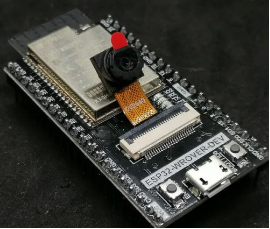
\includegraphics[width=0.6\textwidth]{assets/cap7/7.1.png}
\caption{ESP32 Wroover}
\label{fig:esp32-img}
\end{figure}

\begin{figure}[H]
\centering
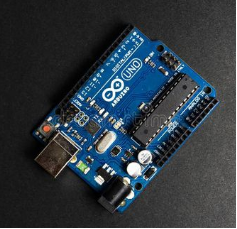
\includegraphics[width=0.6\textwidth]{assets/cap7/7.2.png}
\caption{Arduino UNO}
\label{fig:arduino-img}
\end{figure}

\begin{figure}[H]
\centering
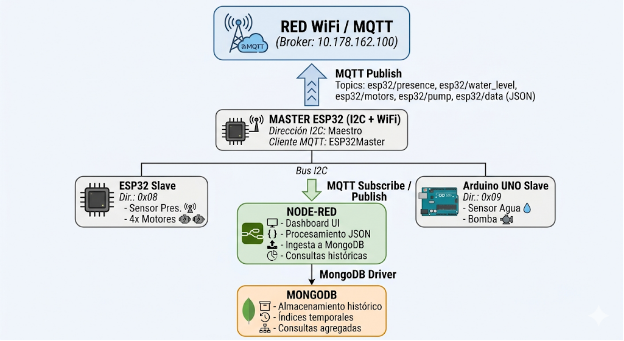
\includegraphics[width=0.95\textwidth]{assets/cap7/7.3.png}
\caption{Esquema de funcionamiento del sistema}
\label{fig:esquema-funcionamiento}
\end{figure}

\textbf{Comunicacion I2C:} Un Maestro (Master ESP32) y dos Esclavos (ESP32 Slave y Arduino UNO Slave) se comunican mediante los pines SCL y SDA. El bus es half-duplex.

\textbf{Topologia MQTT:} El Master ESP32 es el unico productor (publisher). Node-RED actua como suscriptor/consumer principal y se encarga de anadir y consultar la base de datos MongoDB.

\textbf{Flujo de datos principal:}

\begin{figure}[H]
\centering
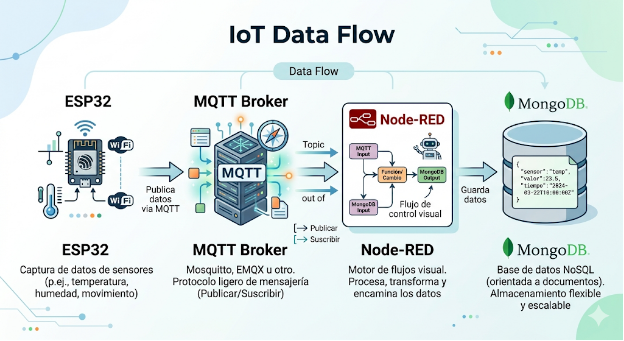
\includegraphics[width=0.95\textwidth]{assets/cap7/7.4.png}
\caption{Flujo de datos principal del sistema}
\label{fig:flujo-datos}
\end{figure}





\section{Protocolo de Comunicacion I2C}

\subsection{Parametros del Bus}

\begin{table}[H]
\centering
\small
\caption{Parametros del bus I2C}
\label{tab:i2c-parametros}
\begin{tabularx}{0.6\textwidth}{@{}lX@{}}
\toprule
\textbf{Parametro} & \textbf{Valor} \\
\midrule
Modo & Maestro-Esclavo \\
Frecuencia & 100 kHz (Standard Mode) \\
Pull-ups & Externas (en hardware) \\
\bottomrule
\end{tabularx}
\end{table}

\subsection{Transacciones}

Transacciones iniciadas por el Master en cada ciclo de \texttt{loop()} (periodo aproximado 200 ms):

\begin{table}[H]
\centering
\small
\caption{Transacciones I2C del ciclo principal}
\label{tab:i2c-transacciones}
\begin{tabularx}{0.85\textwidth}{@{}cclX@{}}
\toprule
\textbf{Orden} & \textbf{Dir.} & \textbf{Bytes} & \textbf{Descripcion} \\
\midrule
1 & 0x08 & 1 & Lectura presencia \\
2 & 0x09 & 2 & Lectura nivel agua + estado bomba \\
3 & 0x08 & 1 & Escritura comando motor (\texttt{'E'} / \texttt{'D'}) \\
4 & 0x09 & 1 & Escritura comando bomba (\texttt{'O'} / \texttt{'F'}) \\
\bottomrule
\end{tabularx}
\end{table}

Las escrituras (pasos 3 y 4) solo se ejecutan si el estado objetivo difiere del ultimo envio exitoso (optimizacion anti-spam).

\subsection{Protocolo de Aplicacion (Comandos)}

\begin{table}[H]
\centering
\small
\caption{Comandos del protocolo de aplicacion I2C}
\label{tab:i2c-comandos}
\begin{tabularx}{\textwidth}{@{}lccc@{}}
\toprule
\textbf{Esclavo} & \textbf{Comando} & \textbf{Valor} & \textbf{Accion} \\
\midrule
ESP32 (0x08) & \texttt{'E'} & Enable & Encender los 4 motores \\
ESP32 (0x08) & \texttt{'D'} & Disable & Apagar los 4 motores \\
Arduino (0x09) & \texttt{'O'} & ON & Encender bomba \\
Arduino (0x09) & \texttt{'F'} & OFF & Apagar bomba \\
\bottomrule
\end{tabularx}
\end{table}

\subsection{Manejo de Errores I2C}

Implementado en el Master:
\begin{itemize}
    \item \textbf{Lecturas:} Hasta 3 reintentos si \texttt{requestFrom} no devuelve la cantidad de bytes esperada.
    \item \textbf{Escrituras:} Hasta 2 reintentos si \texttt{endTransmission} devuelve error (diferente de 0).
    \item Delay entre reintentos: 500 µs (\texttt{delayMicroseconds(500)}).
\end{itemize}


\section{Protocolo de Comunicacion MQTT}

\subsection{Broker y Conectividad}

\begin{table}[H]
\centering
\small
\caption{Configuracion del broker MQTT}
\label{tab:mqtt-broker}
\begin{tabularx}{0.7\textwidth}{@{}lX@{}}
\toprule
\textbf{Parametro} & \textbf{Valor} \\
\midrule
Broker IP & \texttt{10.178.162.100} (produccion/simulacion) \\
Puerto & 1883 \\
Client ID Master & \texttt{ESP32Master} / \texttt{ESP32MasterSim} \\
Keepalive & 60 s \\
\bottomrule
\end{tabularx}
\end{table}

\subsection{Topics Publicados}

\begin{table}[H]
\centering
\small
\caption{Topics MQTT publicados por el Master}
\label{tab:mqtt-topics}
\begin{tabularx}{\textwidth}{@{}lXX@{}}
\toprule
\textbf{Topic} & \textbf{Tipo de Payload} & \textbf{Descripcion} \\
\midrule
\texttt{esp32/presence} & \texttt{"1"} / \texttt{"0"} & Estado de presencia detectada \\
\texttt{esp32/water\_level} & \texttt{"0"} -- \texttt{"100"} & Nivel de agua mapeado \\
\texttt{esp32/motors} & \texttt{"1"} / \texttt{"0"} & Estado de los motores \\
\texttt{esp32/pump} & \texttt{"1"} / \texttt{"0"} & Estado de la bomba \\
\texttt{esp32/data} & JSON consolidado & Mensaje con todos los datos + timestamp + device\_id \\
\bottomrule
\end{tabularx}
\end{table}

\subsection{Formato del JSON Consolidado}

El topic \texttt{esp32/data} transporta un mensaje JSON con la siguiente estructura:

\begin{lstlisting}[caption={Formato del JSON consolidado en esp32/data},label={lst:json-consolidado}]
{
  "device_id": "ESP32-Master",
  "timestamp": "2026-05-26T14:23:04Z",
  "presence": "DETECTED",
  "water_level": 95,
  "motors": "ON",
  "pump": "OFF"
}
\end{lstlisting}

El campo \texttt{timestamp} se envia como string ISO 8601 UTC. Para su correcta ingestion en MongoDB, el receptor (Node-RED) debe convertir la cadena a objeto \texttt{Date} antes de la insercion:

\begin{lstlisting}[caption={Conversion de timestamp en Node-RED},label={lst:conversion-timestamp}]
if (msg.payload && msg.payload.timestamp) {
    msg.payload.timestamp = new Date(msg.payload.timestamp);
}
return msg;
\end{lstlisting}


\section{Maquina de Estados del Sistema}

La logica de control reside integramente en el Master ESP32. Existen 4 estados:

\begin{table}[H]
\centering
\small
\caption{Maquina de estados del sistema}
\label{tab:maquina-estados}
\begin{tabularx}{\textwidth}{@{}lXXX@{}}
\toprule
\textbf{Estado} & \textbf{Descripcion} & \textbf{Motores} & \textbf{Bomba} \\
\midrule
\texttt{STATE\_RUNNING} & Operacion normal & ON & OFF \\
\texttt{STATE\_PUMP\_DELAY} & Espera antes de bombear & OFF & OFF \\
\texttt{STATE\_PUMPING} & Bomba activa & OFF & ON \\
\texttt{STATE\_RECOVERY} & Recuperacion antes de reiniciar & OFF & OFF \\
\bottomrule
\end{tabularx}
\end{table}
Durante \texttt{STATE\_PUMP\_DELAY}, si \texttt{waterLevel >= 35}, se activa la bomba y se pasa a \texttt{STATE\_PUMPING}. Si el nivel es inferior, se salta directamente a \texttt{STATE\_RECOVERY}.








\section{Arquitectura Software y Flujo de Datos}

El sistema implementa una arquitectura software distribuida en tres capas principales:

\begin{enumerate}
    \item \textbf{Capa de Adquisicion}: firmware embebido en los microcontroladores ESP32 y Arduino UNO. El Master ESP32 recopila datos de sensores y estados de actuadores mediante I2C.
    \item \textbf{Capa de Transporte}: el broker MQTT actua como bus de mensajes desacoplado, permitiendo monitorizacion en tiempo real e ingesta de datos historicos.
    \item \textbf{Capa de Orquestacion y Visualizacion}: Node-RED procesa los payloads JSON, distribuye la informacion al dashboard y gestiona la persistencia en MongoDB.
    \item \textbf{Capa de Persistencia}: MongoDB almacena los datos historicos para analisis temporal, generacion de informes y consultas.
\end{enumerate}

\textbf{Flujo de datos principal:} ESP32 (adquisicion) $\rightarrow$ MQTT (transporte) $\rightarrow$ Node-RED (procesamiento/visualizacion) $\rightarrow$ MongoDB (historizacion).


\section{Interfaz, Visualizacion y Dashboard}

El sistema utiliza \textbf{Node-RED Dashboard} como plataforma principal de visualizacion y supervision. Las interfaces graficas permiten visualizar las siguientes variables:

\begin{itemize}
    \item Nivel de agua del tanque (\texttt{water\_level})
    \item Estado de los motores (\texttt{motors})
    \item Estado de la bomba de agua (\texttt{pump})
    \item Deteccion de presencia (\texttt{presence})
    \item Variables recibidas desde los dispositivos ESP32 (identificador, timestamp, etc.)
\end{itemize}

\begin{figure}[H]
\centering
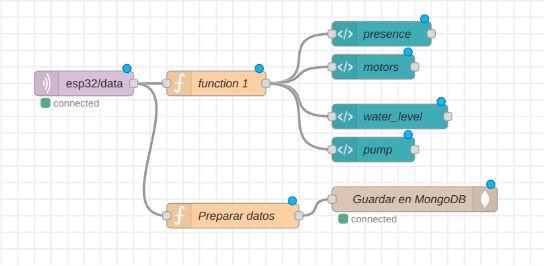
\includegraphics[width=0.8\textwidth]{assets/cap7/7.5.png}
\caption{Dashboard de Node-RED con visualizacion de variables del sistema}
\label{fig:dashboard-nodered}
\end{figure}

\subsection{Flujo de Adquisicion en Tiempo Real}

Flujo principal en Node-RED para suscripcion, procesamiento y visualizacion de datos:

\begin{enumerate}
    \item \textbf{Suscripcion MQTT:} se suscribe al topic \texttt{esp32/data}.
    \item \textbf{Recepcion JSON:} recibe el payload JSON consolidado.
    \item \textbf{Descomposicion:} extrae y procesa cada variable individualmente.
    \item \textbf{Visualizacion:} muestra cada dato mediante elementos visuales del dashboard.
\end{enumerate}

\begin{figure}[H]
\centering
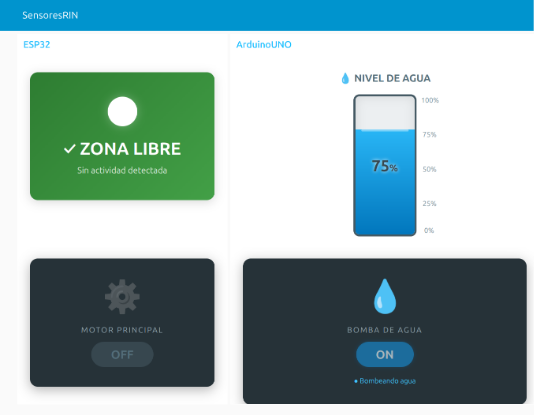
\includegraphics[width=0.8\textwidth]{assets/cap7/7.6.png}
\caption{Flujo de Node-RED para adquisicion en tiempo real}
\label{fig:flujo-nodered-tiempo-real}
\end{figure}

\subsection{Flujo de Analisis Historico}

\begin{figure}[H]
\centering
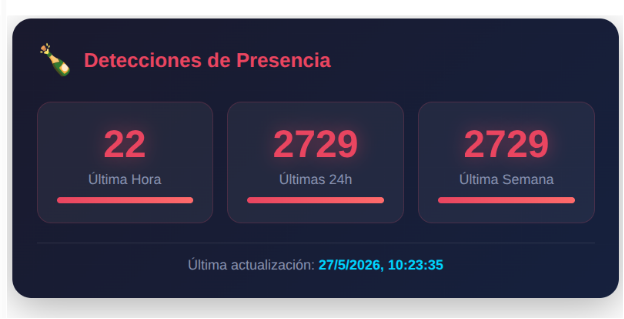
\includegraphics[width=0.8\textwidth]{assets/cap7/7.7.png}
\caption{Dashboard con contador de botellas}
\label{fig:dashboard-botellas}
\end{figure}

Flujo independiente dedicado a la lectura de datos desde MongoDB y presentacion de informacion historica en el dashboard. Proporciona:

\begin{itemize}
    \item Conteo de botellas detectadas (ultima hora, ultimo dia, ultima semana).
    \item Visualizacion simultanea de estadisticas en diferentes ventanas temporales.
    \item Consulta del timestamp de la ultima botella detectada.
\end{itemize}








\section{Diseno de Red Corporativa para la Planta Industrial}

Como parte del proyecto, se ha disenado e implementado en Cisco Packet Tracer un modelo de red corporativa que refleja la infraestructura de comunicaciones que daria soporte a la planta industrial descrita en este capitulo. El objetivo es simular la separacion entre los entornos OT (Operational Technology) e IT (Information Technology) y verificar la conectividad entre todos los elementos del sistema.

\subsection{Arquitectura de red}

La red se estructura en seis subredes, cada una con un proposito especifico:

\begin{itemize}
    \item \textbf{Red de produccion (OT)}: 192.168.10.0/24 — contiene los tres PLCs que controlan las etapas del proceso (control de tanque, llenado y transporte de botellas). Es la unica red con acceso directo a los dispositivos de campo.
    \item \textbf{Red de ingenieria}: 192.168.20.0/24 — estaciones de trabajo para el personal de mantenimiento y supervision tecnica de la linea.
    \item \textbf{Red de administracion}: 192.168.30.0/24 — puestos de gestion y ofimatica de la planta.
    \item \textbf{Red de servidores (DMZ)}: 192.168.40.0/24 — aloja los servidores MQTT Broker, Node-RED y MongoDB, actuando como zona desmilitarizada entre OT e IT.
    \item \textbf{Red de control de calidad}: 192.168.50.0/24 — puesto de inspeccion con camara IP para supervision visual.
    \item \textbf{Red WiFi corporativa}: 192.168.100.0/24 — acceso inalambrico para dispositivos moviles del personal.
\end{itemize}

\begin{figure}[H]
\centering
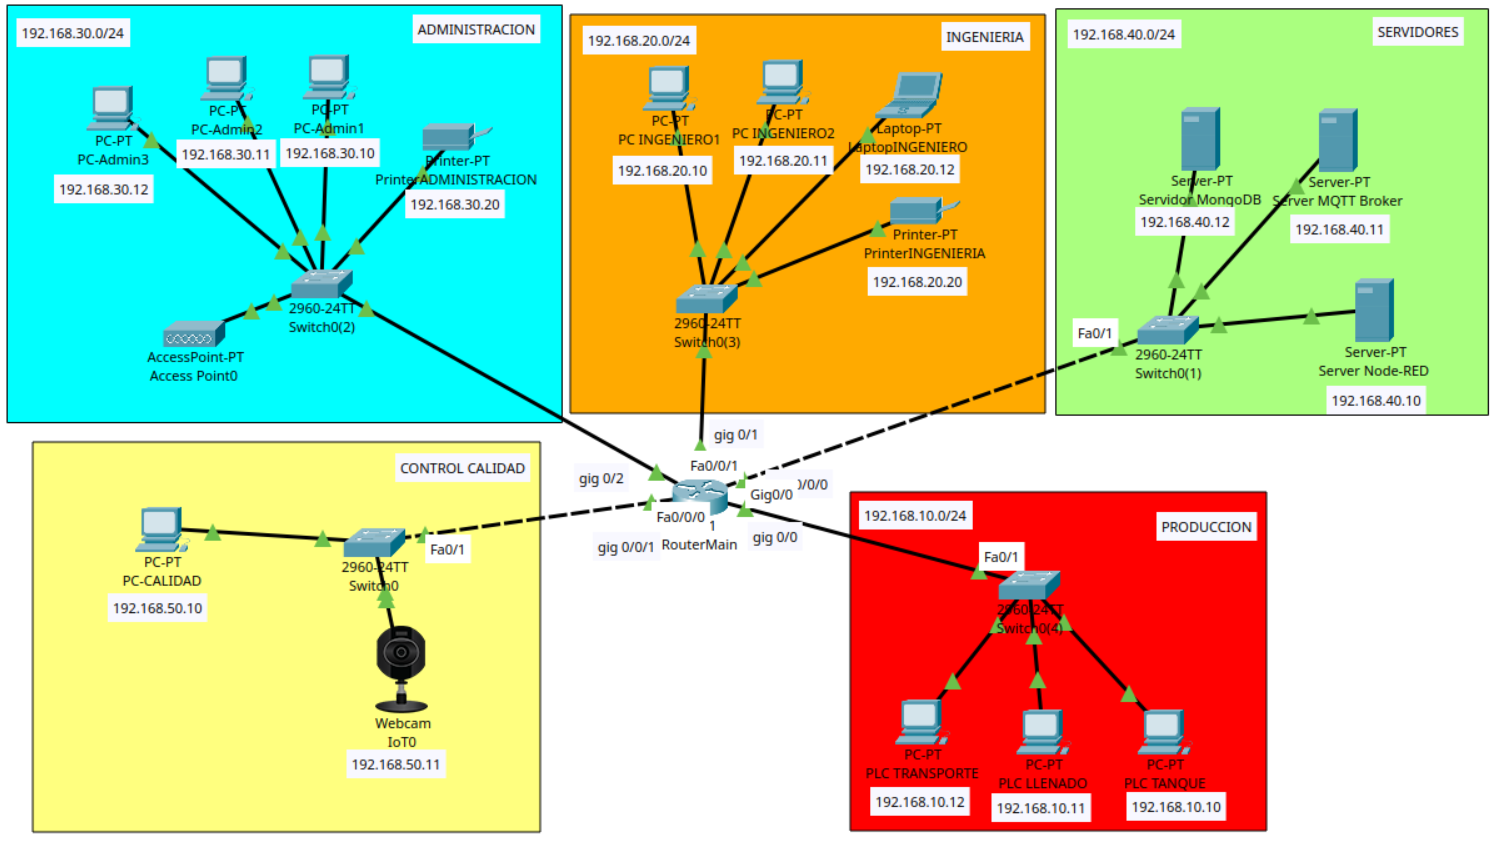
\includegraphics[width=0.85\textwidth]{assets/cap7/7.8.png}
\caption{Topologia de red corporativa en Cisco Packet Tracer}
\label{fig:topologia-packet-tracer}
\end{figure}

\subsection{Componentes de interconexion}

El nucleo de la red es un router Cisco 2911 con las siguientes funciones:

\begin{itemize}
    \item Tres interfaces GigabitEthernet (Gig0/0, Gig0/1, Gig0/2) conectan directamente las redes de produccion, ingenieria y administracion.
    \item Un modulo HWIC-4ESW anade cuatro puertos FastEthernet que, mediante SVIs (Switch Virtual Interfaces), dan servicio a las redes de servidores (VLAN 40) y calidad (VLAN 50) a traves de switches externos.
    \item El router actua como gateway de todas las subredes y encamina el trafico entre ellas.
\end{itemize}

\begin{figure}[H]
\centering
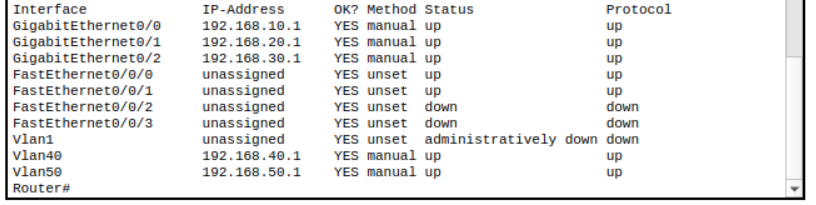
\includegraphics[width=0.8\textwidth]{assets/cap7/7.9.png}
\caption{Configuracion del router con interfaces y SVIs}
\label{fig:router-config}
\end{figure}

\subsection{Esquema de direccionamiento}

\begin{table}[H]
\centering
\small
\caption{Direccionamiento IP de la red corporativa}
\label{tab:direccionamiento-red}
\begin{tabularx}{\textwidth}{@{}lccc@{}}
\toprule
\textbf{Red} & \textbf{Rango} & \textbf{Gateway} & \textbf{Dispositivos} \\
\midrule
Produccion (OT) & 192.168.10.0/24 & 192.168.10.1 & 3 PLCs \\
Ingenieria & 192.168.20.0/24 & 192.168.20.1 & 2 PCs \\
Administracion & 192.168.30.0/24 & 192.168.30.1 & 3 PCs \\
Servidores (DMZ) & 192.168.40.0/24 & 192.168.40.1 & MQTT, Node-RED, MongoDB \\
Control calidad & 192.168.50.0/24 & 192.168.50.1 & PC + camara IP \\
WiFi corporativo & 192.168.100.0/24 & 192.168.100.1 & AP + dispositivos moviles \\
\bottomrule
\end{tabularx}
\end{table}

A continuacion se detalla la funcion de cada departamento dentro de la arquitectura de la planta:

\begin{itemize}
    \item \textbf{Produccion (OT)}: es el nucleo operativo de la planta. Los tres PLCs controlan respectivamente el nivel del tanque de agua, el sistema de llenado de botellas y el transporte de las mismas a traves de las cintas. Esta red debe estar aislada del trafico IT para evitar que incidencias ofimaticas afecten a la produccion. Solo los servidores de la DMZ tienen acceso controlado a ella para la recogida de datos via MQTT.
    \item \textbf{Ingenieria}: destinada al personal tecnico encargado de la supervision, el mantenimiento y la optimizacion de la linea de produccion. Dispone de herramientas de monitorizacion y acceso al dashboard de Node-RED para visualizar el estado en tiempo real de los PLCs y sensores. Tambien es el punto desde el que se realizan actualizaciones de firmware y ajustes de parametros.
    \item \textbf{Administracion}: area de gestion de la planta donde se manejan los indicadores de produccion, la facturacion y la logistica. El personal administrativo accede a los datos historicos del sistema a traves del dashboard, pero no tiene capacidad de escribir comandos sobre los dispositivos OT.
    \item \textbf{Servidores (DMZ)}: zona intermedia que actua como puente entre OT e IT. Alberga el broker MQTT que recibe los datos de produccion, el servidor Node-RED que los procesa y los visualiza, y la base de datos MongoDB que los persiste. Ningun dispositivo externo accede directamente a los PLCs; todo el flujo pasa por esta capa intermedia, lo que anade seguridad y desacopla los sistemas.
    \item \textbf{Control de calidad}: estacion de inspeccion visual donde un operario revisa el producto terminado mediante una camara IP. Los resultados de la inspeccion pueden realimentar el sistema para ajustar parametros de produccion.
    \item \textbf{WiFi corporativo}: proporciona conectividad inalambrica para dispositivos moviles del personal (tabletas, portatiles) dentro de las instalaciones, permitiendo la supervision desde cualquier punto de la planta sin necesidad de estar conectado fisicamente a la red cableada.
\end{itemize}

\subsection{Funcionamiento y flujo de datos}

El flujo de informacion replica el diseno de la memoria tecnica:

\begin{enumerate}
    \item Los PLCs de la red de produccion (OT) adquieren datos de sensores y estados de actuadores.
    \item Estos datos se publican via MQTT hacia el servidor Broker en la red de servidores (192.168.40.10).
    \item Node-RED (192.168.40.11) se suscribe al Broker, procesa los mensajes JSON y los visualiza en el dashboard.
    \item Los datos historicos se persisten en MongoDB (192.168.40.12).
    \item El personal de ingenieria (192.168.20.x) y administracion (192.168.30.x) accede al dashboard a traves del router.
\end{enumerate}

\subsection{Flujo de datos entre departamentos}

El flujo de informacion replica el diseno de la memoria tecnica, cruzando los distintos departamentos de la planta:

\begin{enumerate}
    \item Los PLCs de la red de produccion (OT) adquieren datos de sensores y estados de actuadores en tiempo real.
    \item Estos datos se publican via MQTT hacia el servidor Broker en la red de servidores (192.168.40.10), en la DMZ.
    \item Node-RED (192.168.40.11) se suscribe al Broker, procesa los mensajes JSON y los visualiza en el dashboard.
    \item Los datos historicos se persisten en MongoDB (192.168.40.12) para su consulta posterior.
    \item El personal de ingenieria (192.168.20.x) accede al dashboard para monitorizar y ajustar la produccion.
    \item El personal de administracion (192.168.30.x) consulta los indicadores historicos y las metricas de rendimiento.
    \item El operario de control de calidad (192.168.50.x) registra las inspecciones y puede activar alarmas si detecta anomalias.
\end{enumerate}

\begin{figure}[H]
\centering
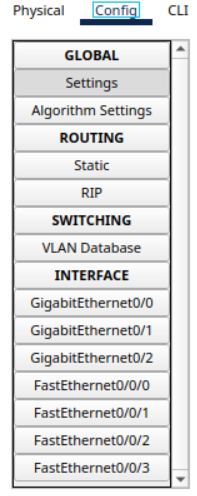
\includegraphics[width=0.27\textwidth]{assets/cap7/7.10.png}
\caption{Tabla de encaminamiento del router}
\label{fig:tabla-rutas}
\end{figure}

El modelo valida que la arquitectura de comunicaciones planteada en la memoria es viable y que la segmentacion en subredes permite aislar el trafico OT del IT, mejorando la seguridad y la gestion de la red industrial.\bigskip


\section{Conclusiones y Recomendaciones Tecnicas}

\begin{enumerate}
    \item \textbf{La arquitectura I2C + MQTT es funcional} y ha sido estabilizada tras las correcciones de anti-spam, manejo de errores y eliminacion de operaciones bloqueantes en ISRs.
    \item \textbf{Las versiones de simulacion permiten validar la logica} sin depender del hardware de campo.
    \item \textbf{El sistema implementa una arquitectura de tres capas completa} (adquisicion, orquestacion/visualizacion, persistencia).
    \item \textbf{Recomendaciones para produccion:}
    \begin{itemize}
        \item Implementar autenticacion TLS en MQTT.
        \item Anadir watchdog software en los esclavos.
        \item Considerar un buffer circular o heartbeat entre Master y Esclavos.
        \item Documentar el esquema electrico completo (pines, alimentacion, pull-ups I2C, adaptacion 3.3V/5V).
    \end{itemize}
\end{enumerate}


\section{Coste de la Instalacion}

El sistema descrito en este capitulo simula un entorno de produccion que, de implementarse en una planta industrial real, requeriria una inversion en equipamiento, sensores, actuadores e infraestructura de comunicacion. A continuacion se desglosan los costes estimados, asumiendo que la planta ya dispone de elementos estructurales como tanques de agua, depositos y obra civil.

\subsection{Componentes considerados}

\begin{itemize}
    \item \textbf{Cintas transportadoras}: se requieren 3 unidades para el transporte de botellas entre etapas, con motorreductores y variadores de velocidad. Coste estimado: 6.000\,\texteuro{} cada una.
    \item \textbf{PLC industrial}: se sustituyen los ESP32 por PLCs compactos (tipo Siemens S7-1200 o similar) para garantizar robustez y estandar industrial. Se necesitan 3 unidades. Coste estimado: 1.200\,\texteuro{} cada uno.
    \item \textbf{Sensores de presencia}: 6 sensores inductivos o fotoelectricos distribuidos en las estaciones. Coste estimado: 150\,\texteuro{} cada uno.
    \item \textbf{Sensor de nivel de agua}: sensor ultrasonico o de presion para el tanque. Coste estimado: 400\,\texteuro{}.
    \item \textbf{Sensorica adicional}: finales de carrera, sensores de posicion y paros de emergencia (10 unidades). Coste estimado: 120\,\texteuro{} cada uno.
    \item \textbf{Actuadores}: electrovalvulas para el sistema de llenado (2 unidades, 350\,\texteuro{} cada una) y bombas industriales (1 unidad, 900\,\texteuro{}).
    \item \textbf{Cableado y canalizaciones}: mangueras apantalladas para senales, cable de potencia para motores y canaletas. Coste estimado: 2.000\,\texteuro{}.
    \item \textbf{Cuadro electrico y armario de control}: incluye fuentes de alimentacion, protectores magnetotermicos, contactores y reles. Coste estimado: 3.500\,\texteuro{}.
    \item \textbf{Infraestructura de red}: switch industrial Ethernet, cableado estructurado y punto de acceso WiFi industrial. Coste estimado: 1.500\,\texteuro{}.
    \item \textbf{Panel HMI}: pantalla tactil para operacion local (7 pulgadas). Coste estimado: 1.800\,\texteuro{}.
    \item \textbf{Puesto de supervision}: ordenador industrial con Node-RED y MongoDB. Coste estimado: 2.500\,\texteuro{}.
    \item \textbf{Integracion y puesta en marcha}: ingenieria de diseno, programacion de PLCs, configuracion de red y pruebas. Coste estimado: 8.000\,\texteuro{}.
\end{itemize}

\subsection{Resumen de costes}

\begin{table}[H]
\centering
\small
\caption{Presupuesto estimado de la instalacion}
\label{tab:presupuesto}
\begin{tabularx}{\textwidth}{@{}lXr@{}}
\toprule
\textbf{Concepto} & \textbf{Descripcion} & \textbf{Importe} \\
\midrule
Cintas transportadoras & 3 uds. & 18.000\,\texteuro{} \\
PLC industriales & 3 uds. (S7-1200 o similar) & 3.600\,\texteuro{} \\
Sensores de presencia & 6 uds. inductivos/fotoelectricos & 900\,\texteuro{} \\
Sensor de nivel & 1 ud. ultrasonico/presion & 400\,\texteuro{} \\
Sensorica adicional & 10 uds. finales de carrera + emergencia & 1.200\,\texteuro{} \\
Electrovalvulas & 2 uds. & 700\,\texteuro{} \\
Bomba industrial & 1 ud. & 900\,\texteuro{} \\
Cableado y canalizaciones & Mangueras, canaletas, conectores & 2.000\,\texteuro{} \\
Cuadro electrico & Armario, protecciones, contactores & 3.500\,\texteuro{} \\
Infraestructura de red & Switch industrial, cableado, WiFi & 1.500\,\texteuro{} \\
Panel HMI & Pantalla tactil 7'' & 1.800\,\texteuro{} \\
Puesto de supervision & PC industrial + software & 2.500\,\texteuro{} \\
Integracion y puesta en marcha & Ingenieria, programacion, pruebas & 8.000\,\texteuro{} \\
\midrule
\textbf{Total estimado} & & \textbf{45.000\,\texteuro{}} \\
\bottomrule
\end{tabularx}
\end{table}

\subsection{Costes de mantenimiento}

Una vez en operacion, la instalacion requiere un mantenimiento anual estimado en los siguientes conceptos:

\begin{itemize}
    \item \textbf{Mantenimiento preventivo}: revision trimestral de sensores, actuadores y cableado. Coste estimado: 1.200\,\texteuro{}/ano.
    \item \textbf{Mantenimiento correctivo}: sustitucion de componentes por desgaste (sensores, reles, contactos). Coste estimado: 800\,\texteuro{}/ano.
    \item \textbf{Actualizacion de software}: parches de seguridad, actualizaciones de Node-RED y MongoDB. Coste estimado: 600\,\texteuro{}/ano.
    \item \textbf{Soporte tecnico}: contrato de asistencia remota y visitas programadas. Coste estimado: 1.500\,\texteuro{}/ano.
\end{itemize}

\textbf{Coste de mantenimiento anual total estimado: 4.100\,\texteuro{}}.


\section{Planificacion}

Para llevar a cabo la implementacion del sistema en una planta industrial real, se propone una planificacion en cinco fases distribuidas en un plazo total estimado de 16 semanas.

\subsection{Fases del proyecto}

\begin{enumerate}
    \item \textbf{Fase de diseno y definicion (semanas 1--3)}:
    \begin{itemize}
        \item Analisis de requisitos funcionales y tecnicos.
        \item Definicion de la arquitectura del sistema y seleccion de componentes.
        \item Diseno del esquema electrico y de comunicaciones.
        \item Elaboracion del presupuesto detallado.
    \end{itemize}
    \item \textbf{Fase de adquisicion e infraestructura (semanas 4--6)}:
    \begin{itemize}
        \item Compra de materiales, sensores, actuadores y PLCs.
        \item Instalacion del cuadro electrico, cableado y canalizaciones.
        \item Montaje de la infraestructura de red (switch, acceso WiFi).
    \end{itemize}
    \item \textbf{Fase de desarrollo e integracion (semanas 7--11)}:
    \begin{itemize}
        \item Programacion de los PLCs (logica de control y maquina de estados).
        \item Configuracion del protocolo I2C entre los nodos.
        \item Implementacion del broker MQTT y los topics de comunicacion.
        \item Desarrollo del dashboard en Node-RED y conexion con MongoDB.
        \item Pruebas unitarias de cada subsistema por separado.
    \end{itemize}
    \item \textbf{Fase de pruebas y puesta en marcha (semanas 12--14)}:
    \begin{itemize}
        \item Integracion de todos los subsistemas y pruebas de conjunto.
        \item Verificacion de la maquina de estados y los flujos de datos.
        \item Pruebas de estres y tolerancia a fallos en la comunicacion I2C y MQTT.
        \item Formacion del personal operario en el manejo del HMI y el dashboard.
    \end{itemize}
    \item \textbf{Fase de operacion supervisada y cierre (semanas 15--16)}:
    \begin{itemize}
        \item Operacion supervisada con acompanamiento tecnico.
        \item Ajustes finos de parametros y temporizaciones.
        \item Entrega de documentacion tecnica y manuales de operacion.
        \item Cierre del proyecto y revision de resultados.
    \end{itemize}
\end{enumerate}

\subsection{Diagrama temporal resumido}

\begin{table}[H]
\centering
\small
\caption{Cronograma del proyecto}
\label{tab:cronograma}
\begin{tabularx}{\textwidth}{@{}lXXXXX@{}}
\toprule
\textbf{Fase} & \textbf{Sem. 1--3} & \textbf{Sem. 4--6} & \textbf{Sem. 7--11} & \textbf{Sem. 12--14} & \textbf{Sem. 15--16} \\
\midrule
Diseno y definicion & $\bullet$ & & & & \\
Adquisicion e infraestructura & & $\bullet$ & & & \\
Desarrollo e integracion & & & $\bullet$ & & \\
Pruebas y puesta en marcha & & & & $\bullet$ & \\
Operacion supervisada y cierre & & & & & $\bullet$ \\
\bottomrule
\end{tabularx}
\end{table}





%%%%%%%%%%%%%%%%%%%%%%%%%%%%%%%%%%%%%%%%%%%%%%%%%%%%%%%%%%%%%%%%%%%%%%%%%%%%%%%
%                                BIBLIOGRAFÍA                                 %
%%%%%%%%%%%%%%%%%%%%%%%%%%%%%%%%%%%%%%%%%%%%%%%%%%%%%%%%%%%%%%%%%%%%%%%%%%%%%%%

\begin{thebibliography}{1}

\bibitem{lemus-poliformat}
   Lemus Zúñiga, G. L.
   \newblock \textit{Material de apoyo a la docencia de Redes Industriales}.
   \newblock Poliformat, UPV, 2026.
   \newblock La totalidad de la información utilizada para la realización de este portafolio proviene de este material.

\end{thebibliography}
\cleardoublepage






%%%%%%%%%%%%%%%%%%%%%%%%%%%%%%%%%%%%%%%%%%%%%%%%%%%%%%%%%%%%%%%%%%%%%%%%%%%%%%%
%                              FIN DEL DOCUMENTO                              %
%%%%%%%%%%%%%%%%%%%%%%%%%%%%%%%%%%%%%%%%%%%%%%%%%%%%%%%%%%%%%%%%%%%%%%%%%%%%%%%

\end{document}